\documentclass[a5paper,
               fontsize=9pt
%                parskip=half,
%                chapterprefix=true,
%                numbers=noenddot
               ]{scrbook}
% \usepackage[utf8]{inputenc}

\usepackage{tocloft}                % Compress TOC and LOF
\usepackage{amsmath,amssymb}        % AMS symbols and environments
\usepackage{physics}
% \usepackage{mathtools}              % More math symbols and environments
\usepackage{fontspec}               % Selecting fonts
% \usepackage{unicode-math}           % Use unicode math font, not TeX
\usepackage[main=english,dutch,italian]{babel}         % Correct hyphenation
\usepackage{booktabs}               % Nicer tables
% \usepackage{xcolor}                 % Colours in text
\usepackage{ccicons}                % Creative Commons icons
\usepackage{pdfpages}               % Insert PDF pages
\usepackage{bookmark}               % Add things in TOC
% \usepackage[hypcap=true]{caption}   % Correctly placed anchors for hyperlinks
\usepackage{scrlayer-scrpage}       % \renewpagestyle Customise head and foot regions
% \usepackage{etoolbox}               % Easy programming to modify TeX stuff
\usepackage{metalogo}               % XeTeX logo
\usepackage{rotating}               % sidewaysfigure
\usepackage{float}
\usepackage[mark]{gitinfo2}
\renewcommand{\gitMark}{\gitAuthorIsoDate{} - \gitFirstTagDescribe}

% From: https://tex.stackexchange.com/a/504869
\newenvironment{abstract}[1]{%
\begin{center}\normalfont\textbf{Abstract}\end{center}
{\begin{quotation}
\textit{\small{#1}}
\end{quotation}}
}{\vspace{1cm}}

% \setlength\columnseprule{.4pt}
\usepackage[round]{natbib}          % Bibliography management
\usepackage{subcaption}
\usepackage{verbatim}               % for \begin{comment} environment.
\usepackage{grffile}                % multidots in file

\usepackage{array}
\newcolumntype{x}[1]{>{\centering\let\newline\\\arraybackslash\hspace{0pt}}p{#1}}
\newcommand{\bss}[2][c]{%
  \begin{tabular}[b]{@{}#1@{}}#2\end{tabular}%
}


\graphicspath{{figures/}, {figures/ch02/}, {figures/ch03/}, {figures/ch_sim_results/}}


\author{Michele Mastropietro}
\title{Simulating Dwarf Galaxies in the Fornax Cluster}
\date{}

\definecolor{greenforlinks}{rgb}{0.09, 0.45, 0.27}
% \PassOptionsToPackage{hyphens}{url}
\usepackage{hyperref}
\makeatletter
\hypersetup{breaklinks=true,
            colorlinks=true,
            allcolors=greenforlinks,
            linktoc=all,
%             pagebackref=true,
            pdftitle=\@title,
            pdfauthor=\@author
           }
\makeatother

% Chapter title style
\makeatletter
\setlength{\fboxsep}{0cm}
\renewcommand*{\@@makechapterhead}[1]{%
  \vspace*{3\baselineskip plus \parskip}
  \makebox{%
    \makebox[\linewidth]{\parbox[c][2cm]{\linewidth}{\if@mainmatter\raggedleft\fi\size@chapter{#1}}}%
    \if@mainmatter%
      \makebox[\marginparsep]{\parbox[c][2cm]{\marginparsep}{\centering\rule{1pt}{2cm}}}%
      \makebox[4cm]{\parbox[c][2cm]{4cm}{\scalebox{5}{\thechapter\autodot}}}%
    \fi
  }%
  \vspace*{1.5\baselineskip plus .1\baselineskip minus .167\baselineskip}
}
\makeatother

% Bullets
\renewcommand{\labelitemi}{►}

% Custom commands
\newcommand{\ie}{i.e.}
\newcommand{\eg}{e.g.}
\newcommand{\cf}{cf.}
\newcommand{\refch}[1]{\hyperref[#1]{Chapter}~\ref{#1}}
\newcommand{\refchs}[1]{Chapters~\ref{#1}}
\newcommand{\refsec}[1]{Section~\ref{#1}}
\newcommand{\refap}[1]{\hyperref[#1]{Appendix}~\ref{#1}}
\newcommand{\reffig}[1]{\hyperref[#1]{Figure}~\ref{#1}}
\newcommand{\reffigit}[1]{\hyperref[#1]{Figura}~\ref{#1}}
\newcommand{\reffignl}[1]{\hyperref[#1]{Figuur}~\ref{#1}}
\newcommand{\reffigp}[1]{\hyperref[#1]{Figure}~\ref{#1} on \hyperref[#1]{page}~\pageref{#1}}
\newcommand{\reftab}[1]{\hyperref[#1]{Table}~\ref{#1}}

\renewcommand{\d}[1]{\ensuremath{\operatorname{d}\!{#1}}}
\newcommand{\pynbody}{\texttt{pynbody}}
% Elements
\newcommand{\hydrogen}{$^1$H}
\newcommand{\helium}{$^4$He}
\newcommand{\heliumthree}{$^3$He}
\newcommand{\lithium}{$^7$Li}
\newcommand{\iron}{Fe}
\newcommand{\Fe}{\text{Fe}}
\newcommand{\magnesium}{Mg}
\newcommand{\Mg}{\text{Mg}}
\newcommand{\Msun}{\text{M}$_{\odot}$}
\newcommand{\Hi}{H\textsc{i}}

% Astronomical terms
\newcommand{\feh}{[\text{Fe}/\text{H}]}
\newcommand{\mgfe}{[\text{Mg}/\text{Fe}]}
\newcommand{\popi}{Pop~I}
\newcommand{\popii}{Pop~II}
\newcommand{\popiii}{Pop~III}
\newcommand{\Popi}{Pop~I}
\newcommand{\Popii}{Pop~II}
\newcommand{\Popiii}{Pop~III}
% \newcommand{\HI}{\ion{H}{i}} % FIXME
\newcommand{\snia}{SN\textsc{i}a}
\newcommand{\snii}{SN\textsc{ii}}
\newcommand{\lcdm}{$\Lambda$CDM}

% Moving Box
\newcommand{\Vp}{\mathbf V_\mathrm p}
\newcommand{\Ap}{\mathbf A_\mathrm p}

% From here: https://tex.stackexchange.com/a/3544
\newcommand{\vect}[1]{\boldsymbol{\mathbf{#1}}}
\renewcommand{\v}[1]{\boldsymbol{\mathbf{#1}}}

% From here: https://tex.stackexchange.com/q/14821/
\renewcommand{\d}[1]{\ensuremath{\operatorname{d}\!{#1}}}


% Figure captions with no indentation
% \setcapindent{0pt}

% List of figures title as "Figures"
\renewcaptionname{english}{\listfigurename}{Figures}
\renewcaptionname{english}{\listtablename}{Tables}

% Add half-title to PDF bookmarks
\makeatletter
\pretocmd{\maketitle}{%
  \if@openright\cleardoublepage\else\clearpage\fi
  \pdfbookmark[0]{Preliminaries}{title}
  \pdfbookmark[1]{Half title}{title}% 
}{}{}%
% Add table of contents to PDF bookmarks
\pretocmd{\tableofcontents}{%
  \if@openright\cleardoublepage\else\clearpage\fi
  \pdfbookmark[1]{Table of contents}{toc}%
}{}{}%
% Add list of figures to PDF bookmarks
\pretocmd{\listoffigures}{%
  \if@openright\cleardoublepage\else\clearpage\fi
  \pdfbookmark[1]{List of figures}{lof}%
}{}{}%
\makeatother

% Font setup
\setmainfont[Path=fonts/,
             Extension=.otf, 
             Ligatures=TeX,
             ItalicFont=*-Italic,
             BoldFont=FeijoaBold,
             StylisticSet=6]{FeijoaMedium}
% \setmonofont[BoldFont=GTPressuraMono-Bold,ItalicFont=GTPressuraMono-LightItalic]{GTPressuraMono-Light}
% \setmathfont{Asana Math}
\newfontfamily\fanciestfont[Path=fonts/,Extension=.otf,Ligatures={TeX,Discretionary}]{FeijoaDisplay}
\newfontfamily\fancyfont[Path=fonts/,Extension=.otf,BoldFont=FeijoaBold,
Ligatures=TeX]{FeijoaDisplay}
\newfontfamily\chapternumberfont[Path=fonts/,Extension=.otf,Ligatures=TeX,Numbers=Lining]{FeijoaDisplay}
\addtokomafont{disposition}{\fancyfont}
\addtokomafont{title}{\fancyfont}
\addtokomafont{chapter}{\fancyfont}
\addtokomafont{chapterentry}{\normalfont\scshape}
\addtokomafont{descriptionlabel}{\normalfont\bfseries}
\addtokomafont{caption}{\footnotesize}

% Levels in table of contents
\setcounter{tocdepth}{1}



\hyphenation{mo-del}

\begin{document}

\frontmatter

% !TEX root = thesis.tex

% Front cover
% \includepdf{cover-front.pdf}

% Half-title
\maketitle


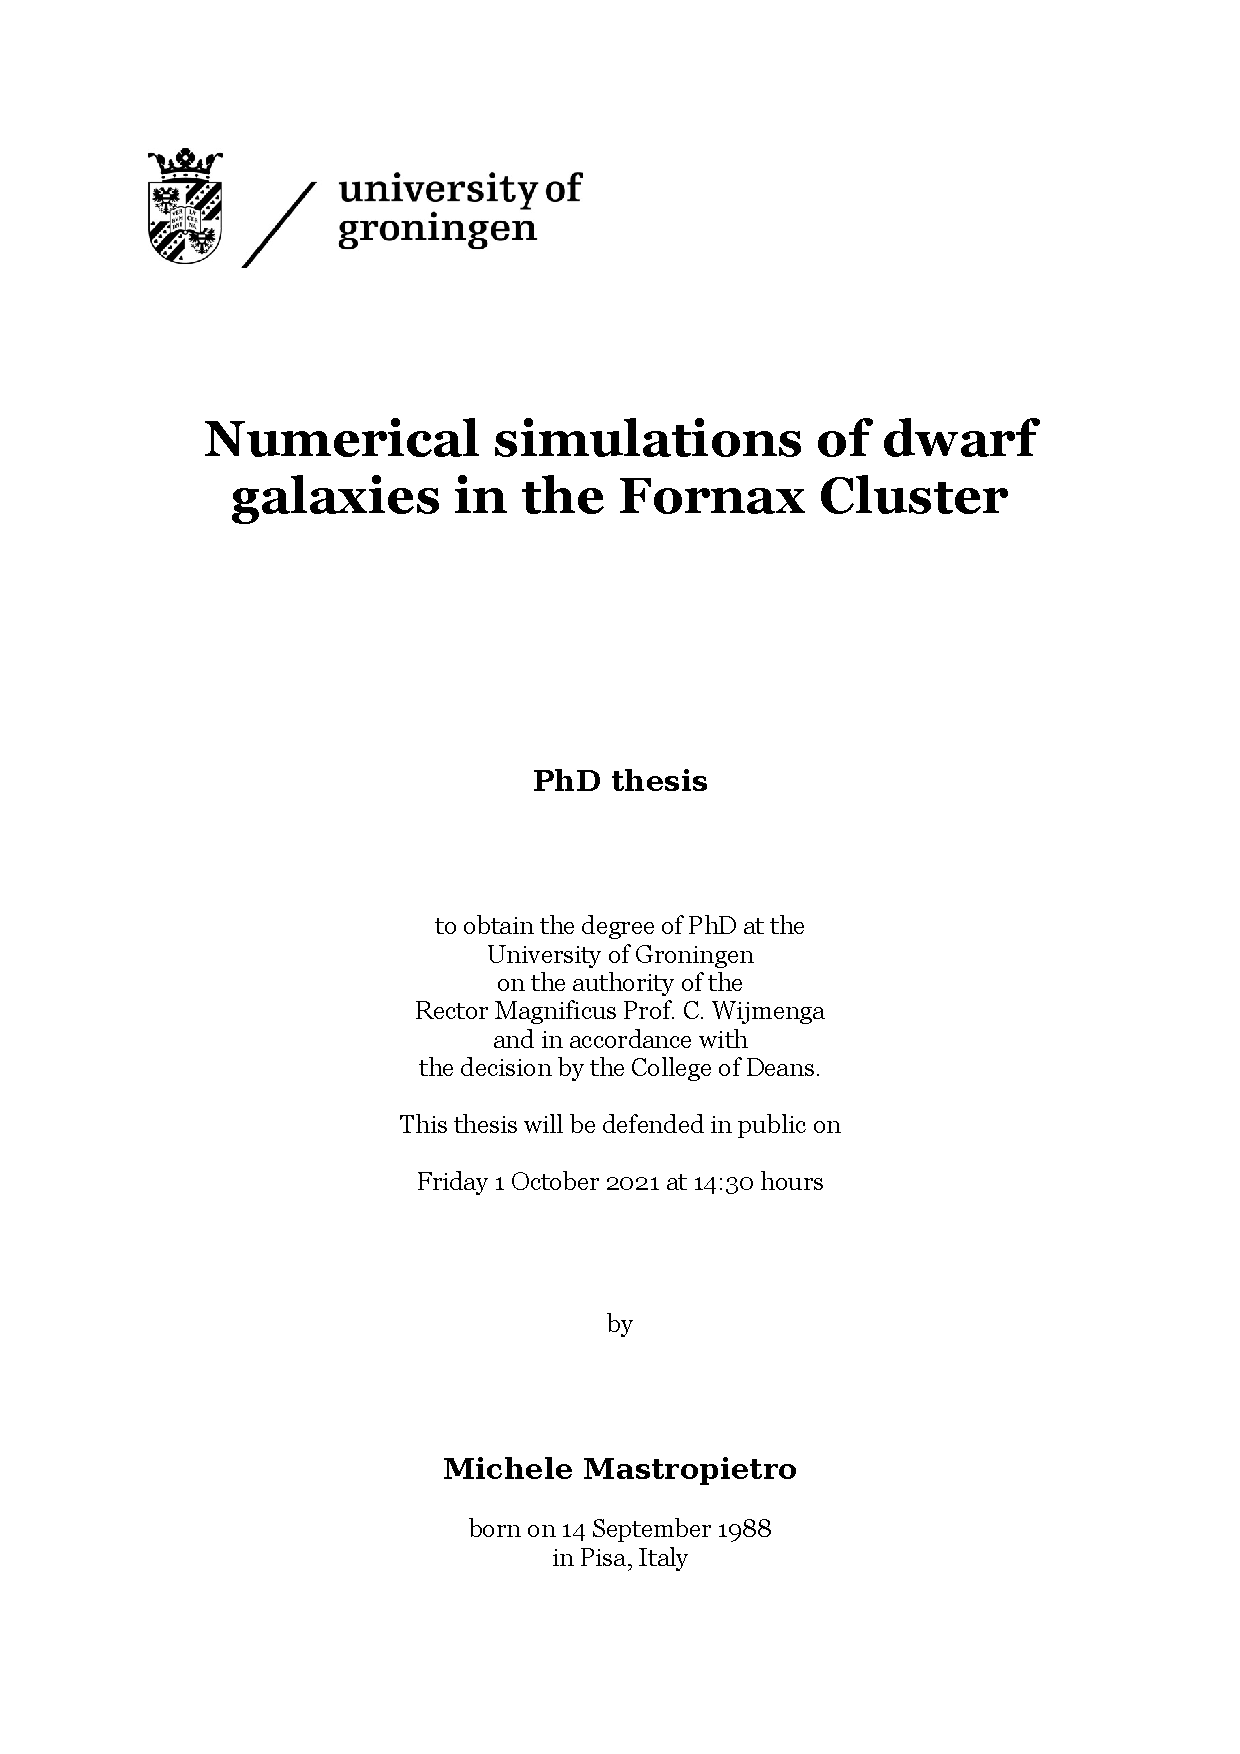
\includepdf[pages=-]{title_page.pdf}


\begin{comment}
% Official title
\begin{titlepage}
\null%
\label{thesis:title}
\vspace{3em}%
\pdfbookmark[1]{Title}{thesis:title}
\begin{center}

%% Skip space as in half-title
\vspace*{4\baselineskip}

%% Print the title.
\makeatletter
{\huge\@title}
\makeatother
\vfill

{\Large Proefschrift}

\medskip

{voorgedragen tot het behalen van \\
de graad van
Doctor in de Fysica en Sterrenkunde}


\medskip

door

\medskip

\makeatletter
{\Large \@author}
\makeatother

\medskip

aan de\\
{\large Universiteit Gent}\\
en aan de\\
{\large Rijksuniversiteit Groningen}\\
% Graduate School of Science and Engineering\\

\end{center}
\end{titlepage}





% Official verso
\clearpage
\thispagestyle{empty}
\null%
\label{thesis:committee}
\vfill
\pdfbookmark[1]{Doctoral committee}{thesis:committee}

% \noindent Members of the examination board:

\medskip\noindent
\begin{tabular}{@{}lll@{}}{Promotors:}\\\\
  \quad{}Prof.\ dr. Sven De Rijcke & Ghent University & (promotor)\\
  \quad{}Prof.\ dr. Michael\ Biehl & University of Groningen & (promotor)\\
  \quad{}Prof.\ dr. Reynier\ Peletier & University of Groningen & (promotor)\\
\\\\
\multicolumn{2}{@{}l@{}}{Composition of the Joint Evaluation Committee:} \\
\\
%   \quad{}Prof.\ dr.\  & chairperson \\
   \quad{}Prof.\ dr.\ Frazer Pearce & University of Nottingham\\
   \quad{}Prof.\ dr.\ Arjen van der Wel & Ghent University \\
   \quad{}Prof.\ dr.\ John McKean & University of Groningen \\
   \quad{}Prof.\ dr.\ Hugues Talbot & Université Paris-Saclay\\
\medskip\noindent
%   \quad{}Dr.\ & University of Groningen\\
% \\
% \multicolumn{2}{@{}l@{}}{Independent members:} \\
% \\
%   \quad{}Prof.\ dr.\ & University of Technology \\
%   \quad{}Prof.\ dr.\ & University \\
%   \quad{}Dr.\& University \\
% \\
% \multicolumn{2}{@{}l@{}}{Other member:} \\
% \\
%   \quad{}Dr.\ & ...\\
\end{tabular}
\end{comment}



% Copyright page
\clearpage
\thispagestyle{empty}
\null%
\label{thesis:colophon}
\vfill
\pdfbookmark[1]{Colophon}{thesis:colophon}
\noindent Written in 2021 by {\makeatletter{\@author}\makeatother}.\\
\textbf{Copyright}~\cczero{} The template for the layout of this thesis was inspired by my colleague Sam Verstocken who used the template of the dissertation of \href{ken.mx}{Ken Arroyo Ohori},
which was released into the public domain using the Creative~Commons~\cczero{}~code.
To view a copy of the \cczero{}~code, visit:\\\url{http://creativecommons.org/publicdomain/zero/1.0/}\\
\textbf{Colophon}
% This thesis was typeset with \XeTeX, Version 3.14159265-2.6-0.99998 (TeX Live 2017/Debian) using the \mbox{{\fanciestfont{}Feijoa}}, \texttt{GT Pressura} and $\mathrm{Asana\ Math}$ typefaces.
Most of the figures were created using \href{http://ipe.otfried.org/}{Ipe} (Copyright © 1993–2020 Otfried Cheong).
The source code of this thesis is available at: \\
\url{https://github.com/elehcim/phd-thesis}\\
\textbf{Cover}
...\\[2ex]
This research was funded by the European Union's Horizon 2020 research and innovation programme under the Marie Sk\l odowska-Curie
% Skłodowska-Curie
grant agreement N.~721463 to the \href{www.astro.rug.nl/~sundial}{SUNDIAL ITN network}.
\begin{figure*}[bh!]
  \centering
  
\includegraphics[width=0.2\textwidth]{EUflag}
\end{figure*}

% Aknowledgements page
\clearpage
\thispagestyle{empty}
\null%
\vfill
\begin{flushright}
  \textit{To my professor of physics:\\
      Mauro dell'Orso\\
      }
\end{flushright}
\vfill

% Aknowledgements page
\clearpage
\thispagestyle{empty}
\null%
\label{thesis:acknowledgements}
  \begin{center}
    {\Large \textbf{Acknowledgements}}\\
  \end{center}
\pdfbookmark[1]{Acknowledgements}{thesis:acknowledgements}
I'd like to thank first of all my professor Sven De Rijcke who believed in me doing a PhD in physics, since the first email in February 2017.
I thank you Sven for showing me what science is, how can it be beautiful and difficult and how it is a fantastic gym to train in deep honesty and integrity.
%As Feynmann said: we've learned from experience that the truth will come out, and it's this type of integrity, this kind of care not to fool yourself.
I've learned from you how to cope with work and life difficulties (especially in these pandemic times) in a very mature and ironic way.
Thank you also for being a mirror for me in our meetings, and always pushing me up even in my down moments.

The SUNDIAL project has been one of the nicest group of people I've ever met.
I'll never forget the high quality of people, their professionalism, attention and kindness for all of us. Thanks to prof. Michael Biehl, for your availability in this joint PhD journey.
Thank you prof. Reynier Peletier, our PI, practically a supervisor for all of us, always available to investigate new ideas with frank and direct attitude: %despite the many obligations and meetings you had to attend:
it's been very inspiring seeing how you live education of young scientists and astronomical research as a calling.
%Thank you Johan, my external mentor, for the interest you showed in my, for being kind and firm showing me how to clearly express.
Thanks to all of the ESRs, the one I had to work directly with: Marco, Abol, Bahar, and each one of the others: Maria Angela, Caroline, Aleke, Alex, Teymoor, Thanh, Mohammad, Shiv, Nushkia, Alan. All the best with your future.
The collaboration among us ESRs has often ended up in very good friendships, and I'll always remember the many memorable moments we lived together (in Naples, La Palma, Ghent...).

I thank my fellow astronomer colleagues at S9, the ones who are there, the ones who left during these years and the ones who just arrived.
I've learned so much from you academically and also how nice and beneficial is a happy work environment like the one you created.
The Belgian ``old guard": Maarten, Seba, Wouter, Peter, Sam, Marjorie, Dries, Robbert, Bert, Ilse, fellow Bert. Thank you for being so welcoming.
Thanks to Ana and Goran for the many moments shared together in our common expats life. Thanks to Francesco and Martina and their family: I've learned so much from you in these years we both were in Gent, much more than you think.
Caro and Pablo, thank you for all the support, deep sharing and friendship.Thank you dear office mates: Caroline, Sara, Anand and Yolan for the discussions and the nice coffee and fruit breaks.
You all have been so nice towards me, it's been an honour to work in the same place as you. Thank you for the many parties, events and dinners and many nice moments lived together.
I also thank the group of the Maxwell Demons: nice people for playing minivoetbal with fantastic team spirit.
Thank you Daniela and Andrea, young fellows of survival in lockdown times: I had so many great moments with you.
Thank you Shivangee, companion of the SUNDIAL adventure, of the office and of the life in Ghent in the happy moments as well as in the difficult times of the PhD far from home: for your constant positive attitude and for always asking how was going on for me and carefully listening. It meant a lot for me.
Thanks to Gianmarco (Jimmy), for showing me many times what true friendship means, and for being at the same time guest and host in our house in Belgium which became yours.
I thank Angelos, a real ``Sam" for me, in the sense of the Lord of the Rings: many times helping me %bringing the sometimes heavy burden of the PhD
and pulling me out of my down moments with frank conversations (is it a perk of living in Frank Baurstraat? ;P), sharing deep insights about life, cooking delicious Greek food (with an appropriate amount of garlic) and being the fuel of many parties and gatherings, with a lot of attention to everyone.

Thanks to my friends at Sint Jacobs in Gent: Davide and Ana (with the newly arrived Bea), Maria and Esteban (with the newly arrived Jose), Caique and Daniela, Valeria, Joshi, Pawel, Eligio and Luca: thank you for the improvised dinners, beers, holidays and deep friendship.
Many thanks to Pinco and the community of the Apostoline for helping me in many ways in these years: thank you for your wisdom and the constant example of free giving (gratuità).

I thank my family: mamma e babbo, for your unbreakable, positive, caring attitude towards me.
%Mi stupisco spesso di come vi siate adattati a fare i genitori di persone adulte con i fatti mostrando una strada siate davvero i genitori che vorrei avere, in tutti questi anni.
Anto for the crystalline confrontations and the enormous sensitivity, Fra for the innumerable funny stories and deep thoughts. Nonna Lida per esserci ed essere una roccia salda per tutti, always.

%Looking back at these years and looking forward for what is waiting for me,
Now that the future opens up after this beautiful adventure of the PhD, I'm on the road to find out a good way to spend my life: each of you is invaluable for orienting me in this. Thank you!

\begin{flushright}
  Gent, 14th September 2021\\Michele Mastropietro
\end{flushright}

% Summary page
\clearpage
\thispagestyle{empty}
\null%
\label{thesis:Summary}
\begin{center}
  {\Large \textbf{Summary}}\\
\end{center}
\pdfbookmark[1]{Summary}{thesis:Summary}

Dwarf galaxies are the most numerous type of stellar systems in the Universe and due to their low mass, they are very sensitive to the surrounding environment.
Because of this, they offer a privileged platform to study and isolate the different physical phenomena affecting galaxy observables.
They can be used as probes to characterize the complex interplay between internal processes and the environment in which galaxies evolve.

We carried out simulations of the evolution of dwarf galaxies falling into a Fornax-like Cluster.
We selected prototypical dwarf galaxies from the MoRIA suite of simulations and injected them one by one on different orbits.
We were interested in following the journey of the galaxies into the cluster and characterize their size, star formation rate, gas and dark matter content, stellar dynamics and evolution, depending on the orbit and the initial mass at the time of orbital injection.
To do so, we implemented the Moving Box simulation technique in our in-house simulation code.
This allows us to simulate the dwarf-cluster interaction at high resolution while keeping an affordable run time.

We found that during infall, generally, galaxies undergo some ``phase transition" happening mainly around pericenter passages.
Some of the galaxies are effectively transformed into Ultra Diffuse Galaxies (UDG) while some others are allowed to be briefly identified as ``jellyfish".
It is therefore possible to hypothesize that the jellyfish phenomenon is a relatively short transitory phase of a dwarf galaxy along its orbit, and it's likely a precursor of the transformation of a dwarf galaxy into an UDG.

Serendipitously we realized that our simulations produce galaxies whose morphology is similar to a galaxy in the Fornax Cluster with a peculiar  \Hi{} tail and an arrow-shaped stellar body oriented in different directions: NGC~1427A.
Multiple formation scenarios have been proposed for this galaxy, but a consensus was still lacking in the literature.
We identified that gaseous and stellar tails pointing in different directions are explainable given that they are subject to different environmental effects (ram-pressure stripping and tidal forces). This idea finds support in our simulations and we developed a procedure to quantitatively assess the properties of simulated galaxies from a catalogue of simulations.
We were also able to provide some falsifiable predictions on the position of the galaxy with respect to the center of the Cluster and its projected orbital direction.

Finally, we have contributed to the development of a technique to study low dimensional-manifolds in the simulations.
We found that the technique can be very useful to isolate the physical properties of filaments in N-body simulations.
In particular we concentrated on the analysis of gaseous tails of simulated jellyfish galaxies with the aim of investigating regions of recent star formation and mixing between the galactic gaseous material and the hot gas of the cluster.


\clearpage
\thispagestyle{empty}
\null%
\begin{center}
  {\Large \textbf{Samenvatting}}\\
\end{center}

%\begin{otherlanguage*}{dutch}
Dwerggalaxieën zijn het talrijkste type sterrenstelsels in het heelal en door hun lage massa zijn zij zeer gevoelig voor hun omgeving.
Daarom bieden zij een bevoorrecht platform om de verschillende fysische fenomenen die de waarneembare eigenschappen van sterrenstelsels beïnvloeden, te bestuderen en te isoleren.
Ze kunnen worden gebruikt als laboratoria om de complexe wisselwerking tussen interne processen en de omgeving waarin galaxieën evolueren te onderzoeken en te karakteriseren.

Wij hebben simulaties uitgevoerd van de evolutie van verschillende dwerggalaxieën die in een Fornax-achtige Cluster vallen.
We selecteerden prototypische dwerggalaxieën uit de MoRIA-simulatiesuite en injecteerden ze één voor één op verschillende banen.
We waren geïnteresseerd in het volgen van de reis van de melkwegstelsels in de cluster en het karakteriseren van hun grootte, stervormingssnelheden, hun inhoud aan gas en donkere materie, hun interne dynamica en hun evolutie, afhankelijk van de baan en de initiële massa op het moment van de injectie in de baan.
Daartoe hebben wij de Moving-Box-simulatietechniek aangepast aan onze noden en geïmplementeerd in onze eigen simulatiecode.
Dit maakt het mogelijk om de dwerg-clusterinteractie met zeer hoge resolutie te simuleren binnen een haalbare totale runtijd.

We ontdekten dat tijdens de inval, over het algemeen, melkwegstelsels enkele faseovergangen ondergaan, die voornamelijk  plaatsvinden bij pericenterpassages.
Sommige van de stelsels  worden getransformeerd in Ultra Diffuse Galaxies (UDG), andere worden kortstondig geïdentificeerd als ``jellyfish''.
Het is daarom mogelijk te veronderstellen dat het ``jellyfish"-fenomeen een relatief korte overgangsfase is van een dwergmelkwegstelsel langs zijn baan, en waarschijnlijk een voorloper is van de transformatie van een dwerggalaxie in een UDG.

Dankzij enige serendipiteit realiseerden we ons dat onze simulaties melkwegstelsels produceren waarvan de morfologie vergelijkbaar is met die van een welbepaald melkwegstelsel in de Fornax Cluster met een eigenaardige  \Hi{} staart en een pijlvormig stellair lichaam die in verschillende richtingen georiënteerd zijn: NGC~1427A.
Voor dit sterrenstelsel zijn meerdere formatiescenario's voorgesteld, maar in de literatuur was er nog geen consensus over.
Wij stelden vast dat gasvormige en stellaire staarten die in verschillende richtingen wijzen verklaarbaar zijn, aangezien zij onderhevig zijn aan verschillende omgevingseffecten (ramdruk en getijdekrachten).
Dit wordt ondersteund door onze simulaties en wij hebben een procedure ontwikkeld om de eigenschappen van gesimuleerde melkwegstelsels kwantitatief te beoordelen aan de hand van een catalogus van simulaties.
We waren ook in staat om enkele falsifieerbare voorspellingen te doen over de positie van het melkwegstelsel ten opzichte van het centrum van de Cluster en zijn geprojecteerde baanrichting.

Tenslotte hebben we bijgedragen aan de ontwikkeling van een techniek om laagdimensionale manifolds in simulaties de bestuderen.
We ontdekten dat de techniek zeer nuttig kan zijn om de fysische eigenschappen van filamenten in N-body-simulaties te isoleren.
In het bijzonder hebben we ons geconcentreerd op de analyse van gasvormige staarten van gesimuleerde ``jellyfish"-sterrenstelsels met het doel regio's van recente stervorming en vermenging tussen het galactische gasachtige materiaal en het hete gas van de cluster te onderzoeken.
%\end{otherlanguage*}

\clearpage
\thispagestyle{empty}
\null%
\begin{center}
  {\Large \textbf{Riassunto}}\\
\end{center}
\begin{otherlanguage*}{italian}
Le galassie nane sono i sistemi stellari più numerosi dell'Universo e, a causa della loro piccola massa, sono molto sensibili all'ambiente che sta loro intorno.
Per questo motivo, offrono una piattaforma privilegiata per studiare e isolare i diversi fenomeni fisici che influenzano le caratteristiche osservabili delle galassie.
Possono essere utilizzati come sonde per caratterizzare la complessa interazione tra i processi interni e l'ambiente in cui le galassie si evolvono.

Abbiamo effettuato simulazioni dell'evoluzione delle galassie nane che cadono in un ammasso con caratteristiche simili a quello della Fornace.
Con alcune galassie prototipali selezionate dalla suite di simulazioni MoRIA e abbiamo messe su una per una su diverse orbite.
È di interesse scientifico seguire il viaggio delle galassie nell'ammasso e a caratterizzare le loro dimensioni, la formazione stellare, il contenuto di gas e materia oscura, la dinamica stellare e la sua evoluzione, a seconda dell'orbita e della massa iniziale al momento dell'iniezione orbitale.
Per fare ciò, abbiamo implementato la tecnica di simulazione chiamata ``Moving Box" nel codice sviluppato nel nostro dipartimento.
Questo ci ha permetto di simulare l'interazione galassia nana ammasso ad alta risoluzione mantenendo un pratico tempo di calcolo.

Abbiamo trovato che durante l'orbita, generalmente, le galassie subiscono alcune ``transizioni di fase" che avvengono principalmente attorno al passaggio per il pericentro.
Alcune galassie vengono effettivamente trasformate in Galassie Ultra Diffuse (UDG), mentre altre possono essere identificate brevemente come ``galassie medusa'' (jellifish).
È quindi possibile ipotizzare che il fenomeno delle galassie medusa sia una fase transitoria relativamente breve di una galassia nana lungo la sua orbita, e che constituisca probabilmente un precursore della trasformazione di una galassia nana in una UDG.

Per una fortuita combinazione, abbiamo notato che le nostre simulazioni producono galassie la cui morfologia è simile a quella di una galassia dell'ammasso della Fornace con una peculiare coda \Hi{} e un corpo stellare a forma di freccia, orientate in diverse direzioni: la NGC~1427A.
Per questa galassia sono stati proposti molteplici scenari di formazione, ma manca ancora un consenso in letteratura.
Abbiamo identificato che le code gassose e stellari che puntano in direzioni diverse sono spiegabili dato che ognuna è soggetta a diversi effetti ambientali (pressione e forze di marea).
Questa idea trova supporto nelle nostre simulazioni.
Abbiamo quindi sviluppato una procedura per valutare quantitativamente le proprietà delle galassie simulate partendo da un catalogo di simulazioni.
Siamo stati anche in grado di fornire alcune previsioni falsificabili sulla posizione della galassia rispetto al centro dell'ammasso e la sua direzione orbitale proiettata.

Infine, abbiamo contribuito allo sviluppo di una tecnica per studiare nelle simulazioni le varietà (manifold) con una dimensionalità bassa.
Abbiamo scoperto che questa tecnica può essere molto utile per isolare le proprietà fisiche dei filamenti nelle simulazioni a N corpi.
In particolare, ci siamo concentrati sull'analisi delle code gassose delle galassie medusa simulate con l'obiettivo di indagare le regioni di recente formazione stellare e di mescolamento tra il materiale gassoso galattico e il gas caldo dell'ammasso.
\end{otherlanguage*}

\cleardoublepage

\tableofcontents

% \listoffigures

% \listoftables


\mainmatter



% !TEX root = thesis.tex

\chapter{Introduction}
\label{ch:introduction}

% \section{Scope of this thesis}
% \label{se:objective}


% !TEX root = thesis.tex

\chapter{Simulations}
\label{ch:simulations}

Numerical simulations have emerged as a new tool to investigate nature, alongside theory and experiments.
This is particularly valid for astronomy where, unlike other laboratory-based disciplines, astronomers may not exert full control over their experiments \citep{Heng2014}.

Computer simulations are essentially a tools to solve complex systems of equations which are intractable with analytic techniques, or only tractable with very coarse level of approximation \citep{Springel2015}.
This allows an unprecedented detailed exploration of the consequences of assumed models for physical systems.
In this sense, the reproduction of observations through computer simulations is a way to validate scientific hypotheses.
The main mathematical model used in galaxy simulations is the fluid model, a branch of continuum mechanics which deals with materials represented as continuous mass as opposed to discrete particles.
In fact, we are not interested in the motion of each molecule in detail, rather we will use a statistical approach . 
In the following we will be dealing with hydrodynamics of fluids, given that the main components of galaxies are successfully described in terms of fluids.

\section{General assumptions}
We will assume the Cold Dark Matter (CMD) paradigm (in a $\Lambda$CDM cosmology), which has gained consensus among the scientific community throughout the years even if up to now, there has been no detection of it \citep[see e.g.][for an extensive and historical overview]{Einasto2010}.
In a dwarf galaxy simulation three kind of fluids are generally taken into account each following different models: dark matter, gas and star. The latter two are so called \emph{baryonic} matter.

Dark matter is hypothesized to consist of small particles that are orders of magnitude smaller than the typical distance scales in our galaxies, so that they constitute a collisionless fluid.
Similarly, the cross section of stars is small compared to galactic scales, and makes them collisionless as well.
Stars, though, affect the gas by pumping energy and metals into their surroundings.
Dark matter and stars are therefore sensitive only to gravity, a weak, conservative, long-range force which is caused by a generally smooth potential.

On the other hand, as we shall see, gas is collisional and its behaviour at any point is affected by short-range interactions, whose modeling requires other assumptions (see below Sections \ref{sec:extended_gas_physics} and \ref{sec:dwarf_models}).

\subsection{Boltzmann Equation - Equations of motion}
The Boltzmann Equation is the general equation which governs the behaviour of a fluid.
From it, the equations of motions can be derived and solved to assess the evolution in time of the fluid.

For simplicity, in this section we assume a single-specie fluid, a generalization to multiple species being straightforward.
For each point of the fluid we would like to know its position and velocity.
Following a statistical approach, at any given time $t$ we can write the distribution function
\begin{equation}
f(\vect x, \vect u, t)
\end{equation}
which describes the number of molecules lying withing a spatial volume $\dd[3]{\vect x}$ about $\vect x$ and with velocity lying in a velocity-space volume $\dd[3]{\vect u}$ about $\vect u$.
These elementary volumes $\dd[3]{\vect x}$ and $\dd[3]{\vect u}$ are finite volume elements which are large enough to contain a very large number of molecules and still small enough to be considered as points when compared to macroscopic dimensions \citep{Huang1987}.
% The distribution function has We can therefore introduce the concept of elementary volume in the 6D phase space $(\vect x, \vect u)$.

% in the elementary volume distribution of the position and velocity of a typical particle
% by its distribution function $f(\vect x, \vect u, t)$ which represents the number density of fluid molecules in the 6D phase space $(\vect x, \vect u)$.
% By multiplying this function with the phase space volume element $\dd[3]{\vect x} \dd[3]{\vect u}$, we obtain the number of particles within this phase space volume element at a given time $t$.
The number density $n(\vect x, t)$ in physical space is obtained by integrating over the velocity:
\begin{equation}
n(\vect x, t ) = \int f(\vect x, \vect u, t) \dd[3]{\vect u}.
\end{equation}
The spatial density is then simply $\rho(\vect x, t) = m_p\,n(\vect x, t)$, where $m_p$ is the mass of the elementary molecule of the fluid.
From this we can define an average value in the position space of a generic quantity $A(\vect x, \vect u, t)$:
\begin{equation}
 \label{eq:df_average}
 \mean A (\vect x, t) = \frac{1}{\rho(\vect x, t)}\int{A(\vect x, \vect u, t)\, m_p\, f(\vect x, \vect u, t) \dd[3] \vect u}
\end{equation}
It is useful to define the averaged (\emph{bulk}) velocity $\vect v$ as:
\begin{equation}
  \vect v(\vect x, t) \equiv \mean{\vect u}(\vect x, t) = \frac{1}{\rho(\vect x, t)}\int{\vect u(\vect x, \vect u, t)\, m_p\, f(\vect x, \vect u, t) \dd[3] \vect u}
\end{equation}
For each elementary spatial volume $\dd[3] \vect x$ we can write the local velocity as the sum: $\vect u = \vect v + \vect w$, where $\vect v$ is the average particle velocity and $\vect w$ a term corresponding to the random movement of the particle with respect to the bulk flow velocity.

In the absence of external forces and assuming the microscopic particles do not collide, the number density in phase space is conserved in time, i.e. no particles are destroyed or created out of nothing in phase space.
This gives immediately the collisionless Boltzmann equation (a.k.a. Vlasov equation):
\begin{equation}
\label{eq:vlasov}
\dv{f}{t}(\vect x, \vect u, t) = \pdv{f}{t} + \vect u \pdv{f}{\vect x} + \vect a \pdv{f}{\vect u} = 0,
\end{equation}
where $\displaystyle \vect a = \dv{\vect u}{t}$ is the acceleration.

In the case of collisions, the Boltzmann equation is modified to:
\begin{equation}
\label{eq:boltzmann}
\dv{f}{t}(\vect x, \vect u, t) = \left.\dv{f}{t}\right|_c,
\end{equation}
where the right term represents discontinuous motion of molecules through phase space because of collisions.

\subsubsection{Euler's equations}
After computing the zeroth, first and second velocity moments of equation \eqref{eq:boltzmann} ---by multiplying by $m_p$, $m_p\vect u$ and $m_p\norm{\vect u}^2$ and by integrating over the entire velocity space--- it is possible to retrieve the equations of hydrodynamics (continuity, momentum and energy) \citep[][and \cite{Vandenbroucke2016} for an extended derivation]{Huang1987}.

In the following we do the assumption that collisions do not create or destroy molecules at a fixed position (they only shift them in velocity space), they conserve momentum and energy.
Consequently in the case of the continuity, momentum and energy equations the right-hand side of equation \eqref{eq:boltzmann} vanishes.
We also neglect diffusive terms (heat conduction and viscous stress tensor) which are often small compared to dynamical effects (an important exception though are shocks for example).

The hydrodynamical equations (a.k.a. Euler equations) are therefore: 
\begin{align}
\label{eq:euler}
 \dv{\rho}{t} &= \pdv{\rho}{t} + \vect v \vdot \grad \rho = - \rho \,\div \vect v, \nonumber\\
 \dv{\vect v}{t} &= \pdv{\vect v}{t} + \left(\vect v \vdot \grad\right) \vect v  = \vect a - \frac{\grad p}{\rho},\\
 \dv{\energy}{t} &= \pdv{\energy}{t} + \vect v \vdot \grad \energy = - \frac{p}{\rho} \div \vect v. \nonumber%\frac{\Gamma - \Lambda}{\rho}
\end{align}
% \begin{equation}
%   \begin{split}
%     \dv{\rho}{t} & + \rho \,\div \vect u = 0\\
%     \dv{\vect u}{t} &+ \frac{\grad p}{\rho} = - \vect a\\
%     \dv{\energy}{t} & + \frac{p}{\rho} \div \vect u = 0
%   \end{split}
% \qquad\qquad
%   \begin{split}
%     &\pdv{\rho}{t} + \grad(\rho \vect v) = 0\\
%     &\pdv{t}(\rho \vect v) + \grad(\rho\vect v \vect v^T + p) = 0\\
% 	&\pdv{t}(\rho e) + \grad (\rho e \vect v + p\vect v) = 0    
%   \end{split}
% \end{equation}
where we defined the pressure as $$p(\vect x, t) = \rho \dfrac 1 3 \trace{(\vect w \vect w^T)} = \rho \dfrac 1 3 \norm{\vect w}^2,$$ assuming an isotropic medium, and the specific internal energy (internal energy per unit mass) as $$\energy(\vect x, t)=\dfrac 1 2 \norm{\vect w}^2.$$ % FIXME Check if this is true
These definitions implicitly fix an equation of state
\begin{equation}
\label{eq:simple_eos}
p = \frac 2 3 \rho \energy. 
\end{equation}
Usually a more general equation of state is assumed $p = (\gamma - 1) \rho \energy$.
For a monoatomic gas: $\gamma = \dfrac{5}{3}$, so equation \eqref{eq:simple_eos} is returned.

Also, the internal energy is related to the temperature via the Boltzmann constants $k_B$:
\[ \energy = \frac {1}{\gamma - 1} \frac{k_B T}{m_p}.\]
For a monoatomic gas $\displaystyle \energy = \frac 3 2 \frac{k_B T}{m_p}$.

% $\Gamma$ and $\Lambda$...

Equations \eqref{eq:euler} describe the dynamics of a perfect monoatomic gas.

\subsection{Gravity}
%We introduce an external force in the Euler equations.
Acceleration in each phase-space position is due to the gravitational field.

In case of self-gravity the source of the acceleration field is the mass density $\rho(\vect x, t)$:
\begin{equation}
 \label{eq:poisson}
 \div \vect a = 4 \pi \,G \, \rho(\vect x, t).
\end{equation}

The gravitational potential $\vect a = \grad \Phi$ can therefore be found through the Poisson's equation:
\begin{equation}
 \label{eq:poisson}
 \laplacian \Phi(\vect x,t) = 4 \pi \,G \, \rho(\vect x, t).
\end{equation}

% For a collisional fluid, a number of approximations are necessary to convert the Boltzmann equation to the Euler equations, but it's still possible.

\section{N-Body systems}
The direct numerical solution of the Boltzmann equation, a non-linear PDE in seven dimensions, is not feasible.
It is interesting to note that in this description the particles have basically completely vanished and have been replaced with a continuum fluid description.
In order to solve the Boltzmann equation (o equivalently the Euler's equations), we represent the fluid by $N$ mass elements (particles), that are conceptually different from the microscopic particles (molecules) constituting the fluid.
The main idea is to discretize the equations above introducing particles.
These are therefore fiducial macro particles that sample the phase-space in a Monte-Carlo fashion \citep{Springel2015}.
Thus, in practice an $N$-body method is a tool for solving the Boltzmann equations.
% In this way then it reduces to solving the gravitational interactions for this $N$-body system \citep{Dehnem2011}.

The equation of motion for particles, following equations \eqref{eq:poisson} can be written as follows:
\begin{equation}
 \vect a_i = -\nabla_i \Phi(\vect x_i),
\end{equation}
\begin{equation}
 \Phi(\vect x_i) = -G \sum^N_{j=1}\frac{m_j}{\sqrt{(\vect x_i-\vect x_j)^2 + \epsilon^2}}.
\end{equation}

where we introduced the softening length $\epsilon$, effectively using a Plummer sphere potential for each particle.
The purpose of the force softening is to avoid the numerical expense that would be needed to integrate the orbits with sufficient accuracy around singularity in the potential.
% Also, we would like to prevent the possibility of the formation of bound particle pairs—they would obviously be highly correlated and hence strongly violate collisionless behavior.

In our simulations we use a softening length of $\epsilon=30$~pc. An estimate of this smoothing length is obtained by requiring that in the gas clouds with the highest density $\epsilon$ is about equal to the average distance between the gas particles. % Mail Sven 24/11/2017
Given that, as we shall see, the in the densest gas clouds star formation occurs at a density of $n\approx100$~amu/cm$^{3}$ (see Section \ref{sec:star_formation}).
When a galaxy is simulated with gas particles of $4000$~\Msun{}, the average distance between the particles in that gas cloud will be of the order of $11$ pc.
So the collapse of the cloud will be followed correctly by the simulation if the softening length is of that order.

\subsection{Smoothed Particles Hydrodynamics}
Smoothed Particles Hydrodynamics (SPH) is a finite volume, Lagrangian particle based numerical method to solve the Navier-Stokes equation of motions for a fluid.
It is a Lagrangian method because the elements carrying information about the fluid move along the fluid itself.
% It is finite volume because it.

A different approach to discretize the fluid domain is to use Eulerian approach, like grid based Adaptive Mesh Refinement (AMR).
Recently, so called \emph{moving-mesh} methods have emerged. They combine both approaches and are more flexible but come with their own difficulties \citep{Springel2010, Shadowfax, Arepo}.
% Several research groups are pushing forward different techniques, sometimes following their own tradition and claiming. 
Usually simple test problems (Sod tube (1D,2D), Sedov blast, Kelvin-Helmholtz instabilities, Noh test, Gresho vortex \citet{Gresho1990}), %TODO fix test
which can be solved analytically, serve as a benchmark for the accuracy of the numerical solution, \citep[e.g. by measuring the distance of the two solution with an L2-norm in the whole domain, ][]{BorrowSphenix}.
Numerical solutions are always a trade-off between accuracy and practicality.
It is interesting to see how a certain gain in accuracy is translated in an increase of \emph{time-to-solution} \citep{Borrow2019}.
%But at the end of the day if we pay attention to the the trend is 

\paragraph{Origin of SPH}
SPH has been originally developed as a \emph{probabilistic} particle method for simulating astrophysical problems \citep{Lucy1977, Gingold1977}\footnote{In a lecture given at Monash University in 2018 \url{https://youtu.be/tAXHCAEgSuE}, prof. Joe Monaghan retrace the origin of the SPH method, recalling that the inspiration for the particle methods to estimate density in fluids comes from David George Kendall, a statistician he collaborated with in Cambridge.}.

A key concept is to relate \eqref{eq:df_average} to SPH formalism.
... Similarity of SPH with eq. \eqref{eq:df_average}...

% In his original treatment \citet{Gingold1977} the probabilities of ... were defined as the expected value
% \begin{equation}
%  E[\rho] = ...% TODO expected values
% \end{equation}

% From J. Monaghan https://www.youtube.com/watch?v=tAXHCAEgSuE
% The general procedure of SPH for solving equations is:
% \begin{itemize}
%  \item Replace the continuum by particles
%  \item Calculate forces on particles
%  \item Follow the motion of the particles
% \end{itemize}
% In statistics the basic interpolant is used to compute probability density except that they do not have mass.
% Instead, for $N$ samples they have the factor $\frac 1 N$.



% Cambridge David Kendall professor of statistics they wanted to calculate probability distributions from samples. They use the same kind of interpolation.

% Problems: Accessing particles (if you have gravity the tree that you build to compute distances and gravity interactions between all the particles can be used in hydrodinamics too.
% The hydro differential equations become a set of ordinary differential equations and (t42:00) and a way to  timestepping is needed.
% Try to construct your discretized equations in a way that it contains the conservation properties of the continuum.

\subsection{Density Estimation from particles ensemble}
A possible choice for the kernel is a Gaussian.
% TODO kernel
It's much more practical to use a finite support approximation of a Gaussian.
The most used for SPH are the Schoenberg  B-spline functions \citep{Schoenberg1988}, generated as the Fourier transform \citep{Price2012}:
\begin{equation}
M_n(r, h) = \frac{1}{2\pi}\int_{-\infty}^{\infty}{\left(\frac{\sin(kh/2)}{kh/2}\right)^n\cos(kr)\d k}.
\end{equation}

By increasing $n$ we obtain progressively better approximations of a Gaussian.
It is convenient to require continuity in at least the first and second derivatives.
Accordingly, the most widely used B-spline for SPH is the lowest order B-spline with this features which is the cubic spline kernel $M_4$:
\begin{equation}
M_4(q) = \frac{1}{\pi h^3} \left\{
\begin{array}{ll}
\frac{1}{4}(2-q)^3 - (1 - q)^{3}, & 0 \le q < 1; \\
\frac{1}{4}(2-q)^3, & 1 \le q < 2; \\
0. & q \ge 2,
\end{array}
\right.
\label{eq:cubicspline}
\end{equation}
where $q=r/h$ is the distance normalized by the smoothing length.

\paragraph{Role of the normalization term}
% TODO probabilistic treatment if it fits
It is somehow striking that the normalization term is not the default in current visualization routines, the only reason being spurious effects when dealing with free surfaces \citep{Price2007}.

\begin{equation}
 A(\vect r) = \dfrac{\sum_j \frac{m_j}{\rho_j} A_j W(|\vect r - \vect r_j|,h)}{\sum_j \frac{m_j}{\rho_j} W(|\vect r - \vect r_j|,h)}.
\end{equation}
...

\section{Dwarf galaxies models}
\label{sec:dwarf_models}
We make use of the MoRIA (Models of Realistic dwarfs In Action) suite of $N$-body/SPH simulations of late-type isolated dwarf galaxies.
They are \textasciitilde$30$ simulations cover the the dwarf galaxy regime (ranging from $10^{6.5}$~\Msun{} to $10^9$~\Msun{} in stellar mass at $z=0$) with different mass assembly histories in a cosmological setting with added \popiii{} feedback \citep{Verbeke2017}.
Isolated proto-galaxies, starting at $z = 13.5$, merge over time along a cosmologically motivated merger tree \citep{Cloet-Osselaer2014}.

MoRIA dwarfs are the sum of multiple researchers work, starting with the implemetation of models for star formation and chemical enrichment \citep{Valcke2008}. 
Then, in addition to the mass, rotation has been found to have a significant influence on the evolution and appearance of dwarf galaxies and their star formation \citep{Schroyen2011}.
Later, the addition of advanced prescriptions for cooling has allowed to increase the resolution when simulating the formation of cold, neutral, high-density clouds suitable for star formation \citep{DeRijcke2013}. %\citep{Verbeke2015}.
MoRIA models could then be used to investigate and reproduce a whole range of observational properties of dwarfs in the field.
Studies have been devoted to characterize their cosmological evolution \citep{Cloet-Osselaer2012}, their star formation evolution \citep{Verbeke2015}, their neutral gas contents and kinematics \citep{Koleva2014}.
This has helped to shed light onto the ``Too big-too fail'' problem \citep{Verbeke2017}.


\paragraph{Physical characteristics} MoRIA dwarfs, have a virial mass at $z=0$ of $M_{200} \approx 10^{10} - 10^{11}$\Msun{}. The dark particle mass is $m_{\mathrm{dm}} = 2 \cdot 10^4$ \Msun{} whereas the baryonic particle mass $m_{\mathrm{b}}$ follows from the relation $\Omega_\mathrm{b}/\Omega_{\mathrm{dm}} = 0.2115$ \citep{Planck2015}.
The typical number of particles is $n_\mathrm{b} = n_{\mathrm{dm}} = 5 \cdot 10^5 - 2 \cdot 10^6$ \Msun{}.

\subsection{Sub-grid models}
For a review see \citet{Verbeke2017, Vandenbroucke2016}.

\paragraph{Star Formation}
\label{sec:star_formation}
Star particles are formed in converging, cold and dense regions of gas.
The following three conditions must be true for a gas particle to be eligible to become a star particle.
\begin{align*}
 T_g &< 15000 \text{~K},\\
 \rho_g &> 100 \text{~amu/cm}^{3},\\
 \div \vect v & < 0.
\end{align*}

The conversion into star particles of gas particles which meet the above conditions is governed by a Schmidt relation \citep{Schmidt1959}
\begin{equation}                                                                              
\dot{\rho}_\star = -\dot{\rho}_g = c_\star \frac{\rho}{t_g}.
\label{eq:schmidt_relation}
\end{equation}
Following \citep{Stinson2006} we assume the characteristic time of formation as the dynamical time $t_g = (4 \pi G \rho_g)^{-1/2}$, whereas $c_\star$ is the star formation efficiency which can be adjusted to match observations.

From this, we can solve the simple differential equation: 
\begin{equation}
\rho_\star = 1 - e^{c_\star \frac{t}{t_g}}.
\end{equation}
We can then use a stochastic method to determine if an eligible gas particle has to be turned in a gas particle.
The Monte Carlo threshold probability of star formation event:
\begin{equation}
P_\star = 1-\exp(-\frac{c_\star \delta t}{t_g}),
\end{equation}
where $\delta t$ is the integration time step.
Given a random number $X \in \mathcal{U}(0,1)$ a star can form if $X < P_\star$.
Several authors \citep{Stinson2006, Revaz2009, Cloet-Osselaer2012} have pointed out that since the star formation is a self-regulating process the star formation rate is weakly dependent on the the choice of $c_\star$ above $0.1$. In our case we use $c_\star = 0.25$.
The new star particle inherits the position, velocity and metallicity of its gas particle progenitor.
In all effects, star particles represent a stellar population with single age and metallicity (SSP, Single Stellar Population) with a Chabrier initial-mass function, \citet{Chabrier2003}.

\paragraph{Stellar feedback}
By \emph{feedback mechanism} it is meant any process that allows to exchange energy, matter and/or momentum between galaxy components. Stars have a huge influence on the interstellar medium (ISM), they pump energy and matter in the surrounding gas mainly enriching ISM with newly formed metals.

The first type of feedback comes from supernovae events. Two main supernovae type are important in simulations. For massive stars, when all the fusion fuel is consumed, gravitation overcome the internal hydrodynamic pressure. The core of the star collapses generating a shock wave which blows away most of the star's outer atmosphere in a massive explosion, leaving behind only a small fraction of its mass, locked up in a remnant (a neutron star or a black hole). This type of core-collapse supernova is called \snii{} (type II supernova).
This type of feedback lasts from the death of the most massive stars of the sampled by the particle's SSP, until the death of the least massive stars which are still capable of going supernova ($>8$ \Msun ): $0.005 - 0.043$ Gyr.
For less massive stars, Type~Ia supernova occurs in a binary star system made by a red giant and a white dwarf.
The gas from a red giant overflows onto a white dwarf and when a critical mass is reached, the white dwarf can no longer be supported and collapses, then rebounds. Neutrinos are thought to play an important role in this expansion \citep{Wongwathanarat2017}.
Because it involves less massive stars and demands a period of steady accretion the feedback of \snia{} is returned $1.54 − 1.87$~Gyr after the birth of the star particle.
Energy injection of \snia{} is delayed by a normally distributed offset-time following \citet{Strolger2004}.
Feedback from supernovae events of type Ia (\snia) and II (\snii) inject $10^{51}$~erg into the surrounding ISM. For more details, the reader is referred to \cite{Valcke2008}.

% Adapted from Simon Driver
%Ia vs Ib depends on if the companion has hydrogen in the atmosphere.

Supernovae events increase the metal content of the ISM. %tracked by Fe and Mg element abundances in gas particles.
In simulations these effects are taken into account by keeping track of two independent metallicities:\feh, \mgfe, corresponding to a fast contribution by the supernova explosions of massive stars, and a slow contribution by the supernova explosions of less massive stars \citep{DeRijcke2013, Vandenbroucke2016}.

A second type type of feedback is stellar wind from young O and B stars.
In simulation stellar wind is taken into account as a uniformly spread energy injection of $10^{50}$ erg in the ISM for $31$~Myr, i.e. from the birth of the star particle until the last massive star ($m = 8$~\Msun) turns \snii{}.


% The stellar population in the star particle is modelled by an initial mass function which tells how many stars are formed with a certain amount of mass. 

\subsection{Extended gas physics}
\label{sec:extended_gas_physics}
\paragraph{Radiative cooling}

\paragraph{Ionization aware equation of state}
In an ideal gas with a single type of constituents, the pressure is given by the equation of state:
\begin{equation}
p = n k_B T
\end{equation}

From \citep[p. 161]{Vandenbroucke2016}, in a multiphase, multicomponent gas with species $S$, this becomes:
\begin{equation}
p = \left(\sum_S n_s + n_e(T)\right) k_BT =\frac{\rho k_B T}{\mean\mu}
\end{equation}
where we introduced the mean constituent mass $\mean\mu$.
This quantity depends on the chemical composition of the gas, its ionization state and the temperature.
As such, following models from \citet{DeRijcke2013}, we can precompute and tabulate it as a function of:
\[\mean\mu = \mean\mu(T, \feh, \mgfe, z, \rho).\]

\subparagraph{Modified equation of energy when considering ionization}
We assume a gas of ${}^1$H with an ionization fraction $x$.
We consider the internal energy to be composed by a (thermal) kinetic part and a ionization part:
\begin{equation}
\label{eq:energy}
\energy = \energy_\text{kin} + \energy_\text{ion}
\end{equation}
The kinetic term (directly linked with the temperature) is defined as
\begin{equation}
\energy_\text{kin} = \frac 3 2 k_B T/ \mean \mu, 
\end{equation}
whereas the ionization energy is
\begin{equation}
\label{eq:energy_ion}
\energy_\text{ion} = \dfrac{\chi_\text H}{m_\text H} x,
\end{equation}
with $\chi_\text H$ and $m_H$ the ionization energy and atomic mass of ${}^1$H.

Assuming no temporal composition changes in the gas (i.e. assuming the gas in ionization equilibrium), the ionization fraction is a function only of the temperature (i.e. the internal kinetic energy) $x = x(T) = x(\energy_\text{kin})$, which allows the temporal derivative of equation \eqref{eq:energy} to be written as:
% \begin{equation}
% \label{eq:du_ion}
% \dv{u_\text{ion}}{t} = 
% \frac{\chi_\text H}{m_\text H} \dv{x}{u_\text{kin}} \dv{u_\text{kin}}{t}
% \end{equation}
% From equations \eqref{eq:u} and \eqref{eq:du_ion}:
% \begin{equation}
% \dv{u_\text{kin}}{t} = \dv{u}{t} - \frac{\chi_\text H}{m_\text H} \dv{x}{u_\text{kin}} \dv{u_\text{kin}}{t}
% \end{equation}
% \begin{equation}
% \dv{u}{t} = \dv{u_\text{kin}}{t} \left( 1+\frac{\chi_\text H}{m_\text H} \dv{x}{u_\text{kin}}\right).
% \end{equation}

\begin{equation}
\dv{\energy}{t} = \dfrac{1}{ 1 + X_\text{ukin}} \dv{\energy_\text{kin}}{t}
\end{equation}
where we defined $X_\text{ukin} \equiv \frac{\chi_\text H}{m_\text H} \dv{x}{\energy_\text{kin}}$.\footnote{The term $X_\text{ukin}$ comes from the the convention of writing the internal energy as $u$. In this thesis we adopted another notation, using $\energy$ to represent the internal energy.}

Instead of evolving the total thermal energy, we can hence evolve the kinetic thermal energy, and adapt the thermal energy equation by applying the correction term $X_\text{ukin}$.
This can be precomputed and tabulated as a function of $(T, \feh, \mgfe, z, \rho)$.

In galaxy simulations this ionization-aware equation of state has the effects of absorbing energy of modeled supernovae explosions.
This has been shown in a Sedov-Taylor blast wave by \citet{Vandenbroucke2013}, where the ionization potential absorbs a significant fraction of the energy injected spent ionizing the gas rather than heating it.
This process can alter the effects of thermal energy injection by supernovae explosions, an important phenomenon to take into account in simulations of galaxies.
% This process can alter the effects of thermal feedback and should not be neglected in simulations of galaxies, where supernovae explosions play an important role.

\paragraph{Ultraviolet background}
UV background (UVB) is a photoionizing radiation due to young UV bright stars or e.g. to QSO whose spectra gets filtered by the Gunn-Peterson effect. It is responsible for preventing gas from cooling in low-mass halos at high redshift \citep{Efstathiou1992, Navarro1997}.
In our simulations, UVB is taken into account in the look-up-tables for gas cooling/heating, for the ionization equilibrium and the mean molecular mass. Its dependence on redshift is implemented following the model by \citet{Faucher-Giguere2009}.
Since in dense neutral region of gas the UVB's photons will be absorbed by outer layers of gas, the gas is self shielding. To capture this effect, in \citet{DeRijcke2013}, the intensity of UVB is modeled with an exponential decay for neutral hydrogen regions with number density $n_{\text{H}\textsc i} \geq 0.007$~amu~cm$^{-3}$.


\section{Moving box}

Using SPH it is computationally challenging to simulate an entire cluster of hot gas while at the same time having the resolution to properly treat the interactions at the interface between the interstellar and intra-cluster medium (or ICM) that cause ram pressure stripping.

\begin{figure}[h]
 \centering
 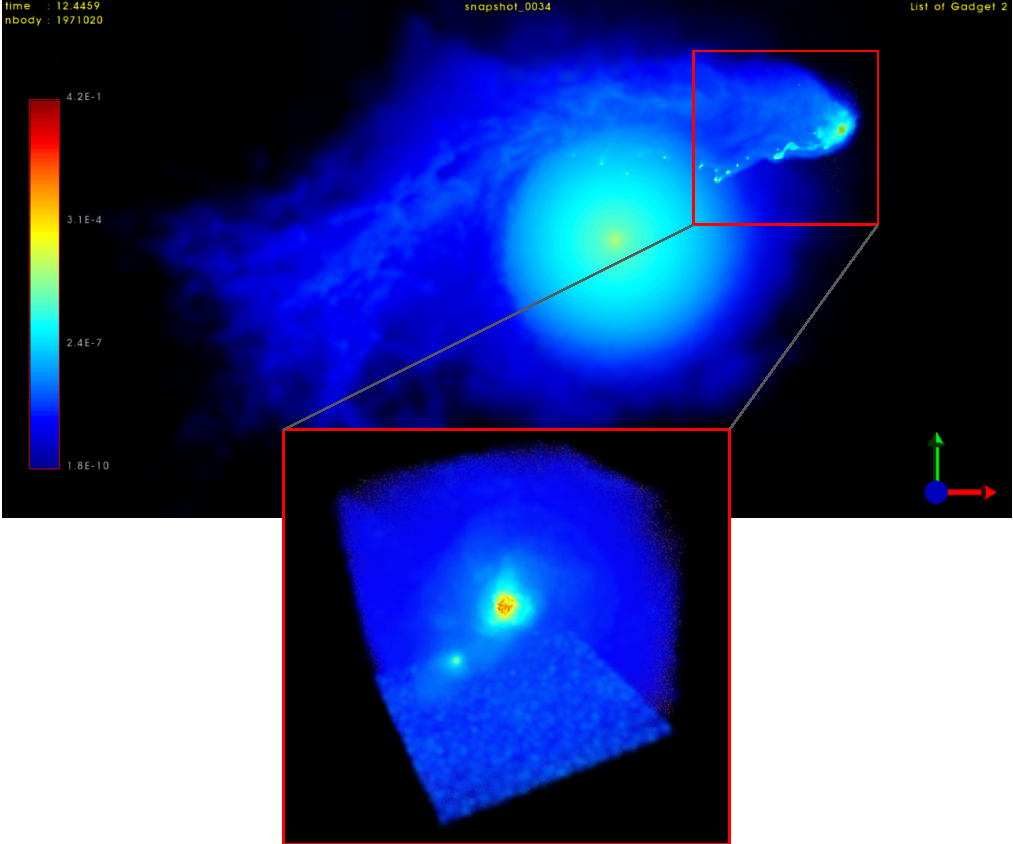
\includegraphics[width=\textwidth]{MovingBox.pdf}
 \caption{An illustration, top panel, of a full fledged simulation of a dwarf galaxy with a Fornax-like cluster. 
 Colors show the gas density \citep[using the \texttt{glnemo2} software][]{Lambert2012}.
 Note the number of particles involved, almost 2 millions.
 The moving box technique, represented in the boxy inset, allows to concentrate resources on the interesting part of the simulation.
 Also, at the dwarf-cluster interface an increased resolution is possible, better resolving the stripping.}
 \label{fig:MovingBox}
\end{figure}

We have opted to use the moving-box technique described by \citet{Nichols2015} and further developed by \citet{Hausammann2019}.
As shown in Figure~\ref{fig:MovingBox}, we enclose the MoRIA dwarf in a $60$~kpc wide moving simulation box, as in a wind tunnel simulation.
Gas is injected from the open ``front" side of the box, which always points in the dwarf's direction of motion. Its density and temperature vary with position, as discussed below in Section \ref{sec:fornax_sim}.
This mimics the hot wind of the cluster halo gas as it streams past the orbiting dwarf galaxy.
Also, additional fictitious forces on the particles are included to take into account the rotation and orbital motion of the moving box.
This allows us to simulate the combined effects of tidal forces and ram-pressure stripping \citep[as studied by][]{Mayer2006} which are acting simultaneously on the dwarf without the necessity of simulating a galaxy cluster worth of intra-cluster gas.
% A typical simulation snapshot contains around $150$k gas particles and $16$k star particles, each with a mass of $4000$~\Msun{}.

\paragraph{Reference frames} 
\begin{figure}[H]
 \centering
 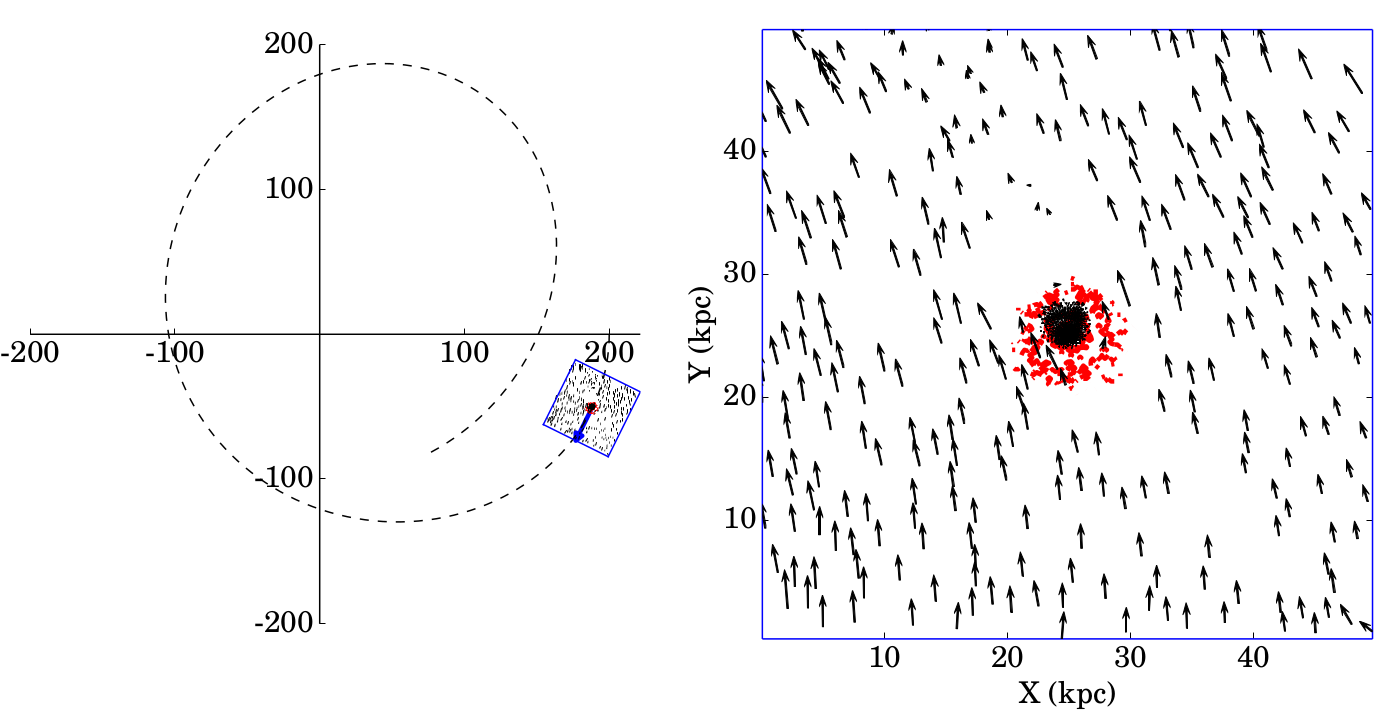
\includegraphics[width=\textwidth]{moving_box_nichols.png}
 \caption{From \citet{Nichols2015}. On the left it is shown the the moving box trajectory. The blue arrow represents the instantaneous box (and therefore dwarf galaxy) velocity.
 On the right, gaseous particles are injected from the bottom side of the box. In red, dark matter density contours, and arrows indicate the wind particles velocity.}
 \label{fig:mb_nichols}
\end{figure}
In a moving box simulation, reference frames have an important roles.
We define the inertial reference frame where the cluster is at the origin.
Relative to that the box moves and rotates, as shown in Figure \ref{fig:mb_nichols}.
To represent the correct rotations, at each moment the quaternion is the moving box is computed.

\subsection{Quaternions}
For completeness, we briefly introduce quaternions algebra.
Following \citet{Graf2008}, a quaternion is a set of four parameters, a real value $q_0$ and three imaginary values $q_1\vect{i},q_2\vect{j},q_3\vect{k}$ with $q_1,q_2,q_3 \in \mathbb{R}$ usually represented as:
\begin{equation}
 \vect q = q_0 + q_1\vect{i} + q_2\vect{j} + q_3\vect{k}.
\end{equation}

The core of quaternion algebra is Hamilton's rule for multiplication of the imaginary units $\vect i, \vect j, \vect k$:
\begin{equation}
 \vect i^2 = \vect j^2 = \vect k^2 = \vect{ijk} = −1,
 \label{eq:hamilton_quaternion}
\end{equation}
from which a complete set of non commutative multiplication rules can be derived.
In fact, noting for example that by left multiplying the last equality in eq. \eqref{eq:hamilton_quaternion} by $\vect i$: $\vect i\,\vect{ijk}=-\vect{jk} = -\vect i$, the product of the imaginary parts are:
\begin{equation}
 \vect{ij} = \vect k, \, \vect{jk} = \vect i, \, \vect{ki} = \vect j.
 \label{eq:hamilton_quaternion_mixed}
\end{equation}

Another useful representation of a quaternion is as a pair $\vect q = (q_0, \vec q)$ of a scalar part $q_0\in \mathbb{R}$ and a vector part $\vec q \in \mathbb{R}^3$ (called also real and imaginary parts, respectively).
\footnote{Only in this section, to distinguish between quaternions and three dimensional-space vectors, we'll use boldface $\vect q$ for quaternions and $\vec q$ for $\mathbb{R}^3$ vectors. In the other sections the difference among the two will be clear from the context.}
Its conjugate~$\conj{\vect q}$ is defined as:
\begin{equation}
 \conj{\vect q} = (q_0, -\vec q),
 \label{eq:conjugate}
\end{equation}
and its norm as:
\begin{equation}
 \norm{\vect q} = \sqrt{q_0^2+q_1^2+q_2^2+q_3^2}.
\end{equation}

From eqs. \eqref{eq:hamilton_quaternion} and \eqref{eq:hamilton_quaternion_mixed} in particular we can write the general formula for the non commutative quaternion multiplication, i.e. given two quaternions $\vect q$ and $\vect p$:
\begin{equation}
 \vect q \vect p = (q_0 p_0 - \vec q \vdot \vec p, \, q_0 \vec p + p_0 \vec q + \vec q \cross \vec p).
 \label{eq:quaternion_multiplication}
\end{equation}
From \eqref{eq:conjugate} it follows that $\vect q \conj{\vect q} = \norm{\vect q}^2 \equiv (\norm{\vect q}^2, \vec 0)$. For unit quaternions ($\norm{\vect q} = 1$), we can write $\conj{\vect q} = \vect q^{-1}$.% because $\vect 1 \equiv (0$.

\paragraph{Quaternions and rotations} Unit quaternions are also called \emph{rotation quaternions}.
They can be used to completely describe a rotation of an angle $\varphi$ around the axis $\vec q$.

Let's consider a unit quaternion $\vect q$. It can be always written as:
\begin{equation}
 \vect q = (q_0, \vec q) = (\cos \frac \varphi 2, \sin \frac \varphi 2\, \hat n), \quad \text{with } \norm{\hat n}=1,
\end{equation}
where $\hat n \equiv \vec q/\norm{\vec q}$ is the versor of $\vec q$.\\
A vector in three-dimensional space $\vec x \in \mathbb R^3$ can be expressed as a \emph{pure quaternion}, a quaternion with no real part: $\vect x = (0, \vec x)$.
% It can therefore multiplied by a quaternion using relation \eqref{eq:quaternion_multiplication}.

The vector $\vec x'$ resulting from the rotation of $\vec x$ of an angle $\varphi$ around the axis $\vec q$ is given by the conjugation operation:
\begin{equation}
\vect x' = \conj{\vect q}\, \vect x \, \vect q 
\end{equation}
where $\vect x' = (0, \vec x')$ \citep[for a proof, see e.g.][sec. 1.4]{Graf2008}.

In the following sections we'll write equations that involve the rotation a quaternion by a vector.
With a slight abuse of notation we will write directly $\vect x' = \conj{\vect q}\, \vect x \, \vect q$, considering that the vector indicated in boldface $\vect x$ should be understood to be the pure quaternion $(0, \vec x)$.% given that it will be clear from the context what is a quaternion (mainly just $\vect q$).

\subsection{Critically damped oscillator}
A slight improvement in our implementation of the moving-box method is the use of a critically damped oscillator for the \emph{ad~hoc} acceleration to keep the galaxy close to the centre of the box.
\begin{equation}
 ...
\end{equation}
We started by noting empirically that for our typical galaxy size a sufficient acceleration is around ...
We want to dump the oscillation as fast as possible, so using a critically damped oscillator with $\zeta... $

A typical behaviour of the \emph{adhoc acceleration} is shown in figure \ref{fig:adhoc}

\begin{figure}
\centering
%  \includegraphics[width=0.8\textwidth]{adhoc.png}
\caption{Adhoc acceleration relative to the total gravitational acceleration of the simulation ID 68 with pericenter 150 kpc.}
\label{fig:adhoc}
\end{figure}


\subsection{Recovering the correct kinematics from a moving box simulation}
\label{sec:corret_kinematics}
Following the convention in \citet{Nichols2015}, capital letters are used for vectors in the inertial frame whereas small letters for vectors in the moving box (rotating frame).
Let $\vect \Omega$ be the angular velocity of the box in the inertial frame, and $\vect q$ the quaternion which at each point in time maps the~$-y$ axis of the rotating reference frame to the direction of the velocity of the box in the inertial frame, $\Vp$.
A vector $\vect X$ in the inertial frame, corresponds to $\vect x = \mathbf q^{-1}\, \vect X \,\mathbf q $ in the rotating frame.

The velocity of the box is measured using a fixed point inside the box, called \emph{pivot}, whose coordinates relative to the box are $\mathbf{x}_{\mathrm p}$ and its velocity and acceleration in the inertial frame relative to the cluster are denoted with $\Vp$ and $\Ap$, respectively.
The \emph{pivot} represents the position in the box of minimal specific energy at the start of the simulation.
From this, $\vect \Omega$ can be computed as 
\begin{equation}
 \vect{\Omega} = {(\Vp\times\Ap)}/{\Vp^2}
\end{equation}
and the angular velocity of the box w.r.t. the rotating frame simply as:
\begin{equation}
\vect \omega = \mathbf q^{-1}\, \vect \Omega\, \mathbf q.
\end{equation}
We can then transform from rotating to inertial coordinates by applying this transformation:
\begin{equation}
\vect V = \Vp + \mathbf q \left(\mathbf v + \vect \omega \times (\mathbf x-\mathbf x_{\mathrm p})\right) \mathbf q^{-1}
\end{equation}
where $\mathbf x$ and $\mathbf v$ are position and velocity of the particle in the rotating frame, respectively, and $\mathbf V$ its velocity in the inertial frame. % For simplicity in the following we don't take into account $\Vp$ since its contribution to the line of sight velocity is negligible.


\section{Simulating the Fornax cluster environment}
\label{sec:fornax_sim}

\subsection{Cluster model}

\subsubsection{Dark matter}
The simulations take into account both ram pressure stripping and the tidal interaction with the cluster.
The latter is simulated as a single spherically symmetric static NFW potential profile \citep{Navarro1996} with mass $M~=~10^{14}$~\Msun{} \citep{Drinkwater2001a}:
\begin{equation}
    \Phi(r) = \frac{G M}{r} \frac{\log(1+r/R_s)}{\log(1 + c) - \frac{c}{1+c}}
\end{equation}
with scale length $R_s = 120$ kpc and $c=8.15$ derived from scaling relations in e.g. \citet{Gentile2004, Wechsler2002}:
\begin{equation}
    c \simeq 20 \left(\frac{M}{10^{11} \text{\Msun{}} }\right)^{-0.13}, \qquad
    R_s = \frac 1 c \left(\frac{M}{\frac 4 3 \pi 200 \rho_c}\right)^\frac 1 3,
\end{equation}
with $\rho_c = 127.3$~\Msun{}~kpc$^{-3}$ the critical density of the universe at $z=0$ for a cosmology with Hubble constant $h=0.67$ and $\Omega_m = 0.31$ \citep{Planck2015}.
The cluster virial radius of the model is $R_{\mathrm{vir}} = c R_s = 978$~kpc.

\subsubsection{ICM} \label{sec:ICM}
Following \citet{Paolillo2002}, we use the superposition of three spherically symmetric beta-models, $\rho(r) = \rho_0 (1 + (r/r_0)^2 )^{-3\beta/2}$, to construct the gas density profile in the Fornax cluster, as shown in Figure \ref{fig:profiles}.
They identify three contributions to the hot gas distributions: a central component (dominating for $r<5''$), coincident with the optical galaxy NGC1399; a less dense and more extended galactic component ($50''<r<400''$); and a cluster component ($r>400''$).
We assume the gas to be in hydrostatic equilibrium with temperature $T(r)$ computed as:
\begin{equation}
   T(r) = \frac {m_p}{k_B \rho(r)} \int_r^\infty \rho(r') \frac{GM(r')}{r'^2} \mathrm{d} r'
\end{equation}
where $M(r)$ is the mass of the gas, stars and dark matter beyond radius $r$, $m_p$ is the proton mass, $G$ and $k_B$ the gravitational and Boltzmann constants.

\begin{figure}
\centering
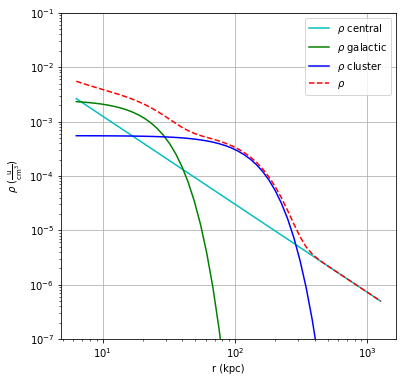
\includegraphics[width=0.8\textwidth]{PaolilloRho.png}
\caption{Gas density profile $\rho(r)$ of the  Fornax Cluster model as a superposition of three beta models from measurements described in \citet{Paolillo2002}, from which we also adopt the nomenclature for the different beta models.
}
\label{fig:profiles}
\end{figure}

These two radial profiles allow us to inject particles with the proper density and temperature in the moving box, hence recreating the environmental condition of the cluster as the dwarf orbits through it.

\subsection{Simulation parameters}
We carried out a set of simulations starting from five MoRIA models of late-type galaxies taken at $z = 0.5$.
The overall goal in setting up the simulations is to study the evolution of late-type galaxies in a cluster environment.
The choice of the redshift of infall has been motivated by the fact that the number of red dwarfs in the Fornax cluster has increased significantly since $z = 0.5$ \citep{Stott2007, DeRijcke2010}.
That indicates that the conversion of late-type to early-type dwarfs (and hence the acquisition of late-type dwarfs by clusters) is probably a recent event.

We selected dwarfs models covering the stellar mass range of $10^{7.5}-10^{9}$ and we injected each of them on 5 different orbits with pericenter distances of $50, 100, 150, 200,$ and $300$~kpc and with a fixed apocenter of 800 kpc.
The starting point of the infall is always at a radial distance of 600~kpc.
We chose a lower radial distance of the starting position w.r.t. the virial radius given the very low cluster density in that region and the low orbital velocity of the dwarf near apocentre.
In this way, simulations could be concentrated on the infall and the pericenter passages of the simulated dwarfs.
We evolved the galaxies for $5.5$~Gyrs up to $z=0$.
The initial stellar masses are reported in Table \ref{tbl:sim}.
All simulations presented in this paper, at time of injection have exponentially declining SB profiles with Sersic index around 1.0.
Every $10$~Myr a snapshot is saved, yielding around 560 snapshots for each simulation.
This high snapshot cadence has proven to be important for the following analysis (see Section \ref{sec:morphological_quest}).
Adhering to the simulation goal of following the evolution of a gas-rich late-type dwarf in a Fornax-like cluster, the initial snapshot of the most massive dwarf (ID 41) has been taken at $z=0.4$ because at $z=0.5$ it was still undergoing a major merger event.
This is equivalent to having this galaxy falling into the cluster more recently.
No sizeable effect has been noted in simulations results highlighting a different behaviour with respect to the other galaxies \citep[which underwent their last merger before infalling to the cluster at $z=0.5$, see e.g.][]{Cloet-Osselaer2014}.
This has had the only implication of a lower number of snapshots used in the technique explained in Section \ref{sec:morphological_quest}, but, as we shall see in the following, given that first pericenter passage turns out to be the most significant orbital phase, no notable bias is expected.

\begin{table}
\centering
\footnotesize
\begin{tabular}{cx{1.3cm}x{0.5cm}x{0.8cm}x{0.7cm}x{0.4cm}x{1.4cm}}
\toprule
Sim ID & $\log_{10}$(M$_\star$)\newline(M$_\odot$) & $R_e$ \newline (kpc) & $\sigma_\star$ \newline (km/s)\\
\midrule
  62 &  6.66 &  0.8 &  11.4 \\%&  -11.8 &  0.5 &  25.8 \\
  71 &  7.58 &  1.9 &  21.9 \\
  68 &  7.96 &  2.6 &  15.6 \\
  69 &  8.04 &  2.3 &  24.6 \\
  41 &  8.78 &  1.7 &  30.4 \\
\bottomrule
\end{tabular}
\caption{Features at time of infall ($z=0.5$) of the selected MoRIA dwarf models used in this work}
\label{tbl:sim}
\end{table}


% !TEX root = thesis.tex

\chapter{Simulation results}
\label{ch:sim_results}

\section{Introduction}


\begin{sidewaystable}
 \centering
 \footnotesize
 \begin{tabular}{lx{0.8cm}x{1.4cm}x{0.7cm}x{1cm}x{0.8cm}x{0.8cm}x{0.7cm}x{1.9cm}}
\toprule
name & peric. \newline (kpc) & $\log_{10}$(M$_\star$) \newline (M$_\odot$) & $R_e$ \newline (kpc) & $\sigma_\star$ \newline (km/s) & M$_V$ \newline (mag) & M$_{r'}$ \newline (mag) & $n$ & $\bar{\mu}_{e,r'}$ \newline (mag/arcsec$^2$) \\
\midrule
  62 &                        50 &                                        6.50 &                  1.6 &                            6.7 &                 -9.7 &                   -10.1 & 1.1 &                                         28.7 \\
  62 &                       100 &                                        6.57 &                  1.6 &                            8.0 &                 -9.9 &                   -10.2 & 1.0 &                                         28.5 \\
  62 &                       150 &                                        6.59 &                  1.6 &                            9.1 &                 -9.9 &                   -10.2 & 1.4 &                                         28.6 \\
  62 &                       200 &                                        6.59 &                  1.7 &                            8.3 &                -10.0 &                   -10.3 & 1.2 &                                         28.5 \\
  62 &                       300 &                                        6.64 &                  1.7 &                            8.6 &                -10.1 &                   -10.4 & 1.0 &                                         28.2 \\
  71 &                        50 &                                        6.26 &                  6.7 &                           21.6 &                 -9.5 &                    -9.8 & 0.0 &                                         31.8 \\
  71 &                       100 &                                        6.82 &                  6.2 &                            6.5 &                -10.9 &                   -11.2 & 0.5 &                                         30.5 \\
  71 &                       150 &                                        6.79 &                  6.4 &                            0.8 &                -10.7 &                   -11.0 & 0.5 &                                         30.5 \\
  71 &                       200 &                                        6.85 &                  6.9 &                            0.8 &                -11.0 &                   -11.3 & 0.2 &                                         30.4 \\
  71 &                       300 &                                        6.85 &                  7.2 &                            1.8 &                -11.0 &                   -11.4 & 0.2 &                                         29.7 \\
  69 &                        50 &                                        6.81 &                  7.6 &                            1.6 &                -10.6 &                   -11.0 & 0.2 &                                         30.7 \\
  69 &                       100 &                                        7.53 &                  7.1 &                           17.8 &                -12.5 &                   -12.9 & 0.1 &                                         28.4 \\
  69 &                       150 &                                        8.05 &                  4.3 &                           11.6 &                -14.2 &                   -14.4 & 0.3 &                                         26.8 \\
  69 &                       200 &                                        8.34 &                  3.3 &                           18.4 &                -15.0 &                   -15.3 & 1.0 &                                         25.0 \\
  69 &                       300 &                                        8.42 &                  1.8 &                           23.9 &                -15.5 &                   -15.7 & 0.9 &                                         23.5 \\
  68 &                        50 &                                        6.27 &                  8.0 &                            nan &                 -9.1 &                    -9.4 & 0.0 &                                         32.3 \\
  68 &                       100 &                                        6.85 &                  7.3 &                            2.5 &                -10.6 &                   -10.9 & 0.1 &                                         31.2 \\
  68 &                       150 &                                        6.85 &                  7.3 &                            nan &                -10.6 &                   -10.9 & 0.1 &                                         31.2 \\
  68 &                       200 &                                        7.02 &                  7.4 &                            nan &                -11.4 &                   -11.7 & 0.1 &                                         30.0 \\
  68 &                       300 &                                        8.09 &                  3.8 &                           11.5 &                -14.5 &                   -14.8 & 0.8 &                                         26.2 \\
  41 &                        50 &                                        8.93 &                  3.5 &                           16.5 &                -16.2 &                   -16.5 & 1.0 &                                         23.9 \\
  41 &                       100 &                                        8.94 &                  2.5 &                           26.0 &                -16.4 &                   -16.7 & 1.0 &                                         23.0 \\
  41 &                       150 &                                        8.99 &                  1.7 &                           28.5 &                -16.6 &                   -16.8 & 0.8 &                                         22.2 \\
  41 &                       200 &                                        8.97 &                  2.2 &                           29.4 &                -16.6 &                   -16.8 & 0.8 &                                         22.5 \\
  41 &                       300 &                                        9.04 &                  1.8 &                           33.7 &                -17.0 &                   -17.2 & 0.7 &                                         21.8 \\
\bottomrule
\end{tabular}

 \caption{Features of the selected MoRIA galaxies at $z=0$.} \label{tbl:galaxies}
\end{sidewaystable}


\paragraph*{Radial period}
Pericenter passages, as explained in the following, are important moments for the life of the simulated dwarf.
In order to compare different orbits, we normalise the simulation time by the orbital radial period $T_r$, i.e. the time between two pericenter passages, \citep[p.~146]{BinneyTremaine2008}:
\begin{equation}
    T_r = 2 \int^{r_a}_{r_p} \frac{\d r}{\sqrt{2\left[E-\Phi(r) \right] - J^2/r^2}}
    \label{eq:radial_period}
\end{equation}
where $r_p, r_a$ are the pericenter and apocenter distance respectively, $E$ and $J$ the orbital energy and angular momentum per unit mass, $\Phi(r)$ the potential at radius $r$ of the NFW halo around which the galaxy is orbiting.

By defining the time of pericenter passage as $t_p: r(t_p) = r_p$, we can introduce the normalized time:
\begin{equation}
\tau = \frac{t-t_p}{T_r},
\end{equation}
which is~$0$ or $1$ for first or second pericenters respectively,~and~$0.5$ for apocenter passages.

% We begin with following one galaxy in its journey around the cluster.
In the following we will compare the effects of orbit and initial mass using the set of 25 simulations we have carried out.


\paragraph*{Tidal radius}
As we shall see, the cluster gravitational potential is able to strip material from the galaxy. Some of the simulations, depending on the orbit they are on, will become gravitationally unbound dominated by the cluster potential.
We chose to define the event of becoming unbound using the condition on the tidal radius \cite{King1962}: namely when it becomes greater than the effective radius.
This physically implies that orbits of the stars in the outskirt of the galaxy are influenced by the cluster potential more than the galactic halo potential. 
Tidal radius $r_t$ is computed as following.
\begin{equation}
r_t = r \sqrt[3]{\frac{M_g}{M_c(r) (3+e)}}
\label{eq:tidal_radius}
\end{equation}
where $e = (r_a - r_p) / (r_a + r_p)$ is the eccentricity of the orbit computed, $r_a$, $r_p$ the apocenter and pericenter radii respectively; $M_c(r)$ is the enclosed cluster mass at radius $r$, and $M_g$ the instantaneous total mass of the galaxy.
As a convention we measure the galaxy mass as the total mass (baryonic and dark matter) within 10~kpc from the center of the galaxy.

In Figure \ref{fig:tidal_radius} we show an example of $r_t$ evolution along the orbit.
We define a galaxy to become unbound when the condition 
\begin{equation}
    R_e > r_t
\label{eq:tidal_radius_condition}
\end{equation}
first occurs.
%Galaxies on a radial orbits will undergo disruption more easily.
\begin{figure}
\centering
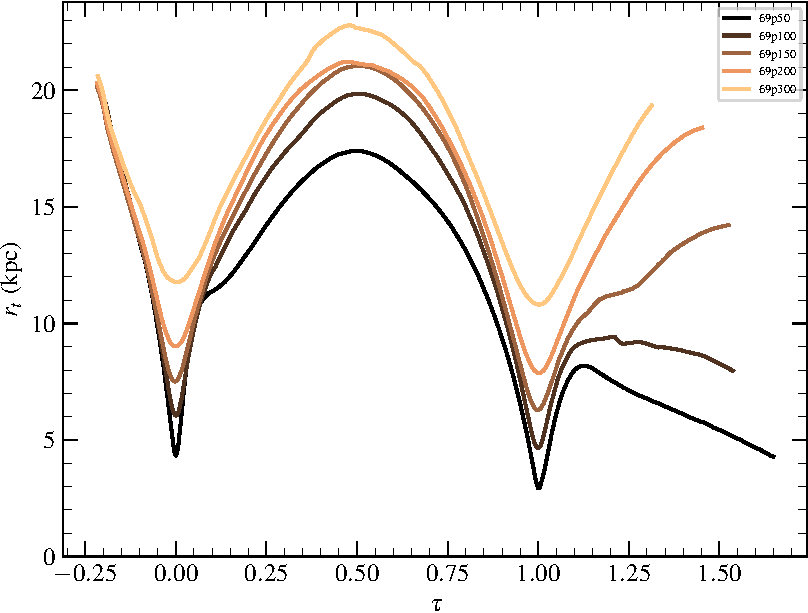
\includegraphics[width=\textwidth]{14.0_tidal_radius.pdf}
\caption{Evolution of the tidal radius for the simulations ID 68.}
\label{fig:tidal_radius}
\end{figure}

\section{Becoming an Ultra Diffuse Galaxy (UDG)}
\label{sec:UDG}

Faint Low Surface Brightness (LSB) galaxies with $R_e > 1$ kpc have been detected in galaxy clusters since the 1980s \citep[e.g.][]{Sandage1984}.
% See Wittmann  https://www2.mpia-hd.mpg.de/homes/galClusters_2017/slides/Ringberg2017_presentation_Wittmann.pdf

% Wittmann2017 studies LSB in Perseus
LSB galaxies are defined as having \citep{Venhola2017}:
\begin{equation}
\begin{cases}
 \mu_{0,r'} > 23 \mbox{ mag/arcsec}^2\\
 M_{r'} > -19
\end{cases}
\end{equation}

In 2015 \citet{VanDokkum2015} introduced a size criterion to distinguish between more compact 'normal' dwarfs \citep{Sales2021}:
UDG are therefore defined as large ($R_e > 1.5$~kpc) low surface brightness galaxies.
%($\bar\mu_{r',e} > 24$~mag/arcsec$^2$).

The majority of studies indicate that they have the properties of large dwarf galaxies \citep{Sandage1984, Roman2017, Venhola2017, Saifollahi2021}.
Three main mechanisms are hypothesised as possible formation scenarios for UDGs \citep{Rong2020}:
dwarf galaxies which undergo strong tidal stripping \citep{Venhola2017, Carleton2018, Rong2020a},
gas outflows driven by stellar feedback with extended dark matter halo and faint and diffuse stellar component \citep{DiCintio2017, ManceraPina2019},
or failed $L^*$ galaxies in high mass dark halos with ceased star formation in the early universe.

Some UDGs have earlier been identified as disrupted early-type galaxies.
\citet{Koch2012} is indeed able to reproduce a typical S-shape tidal tailed UDGs HCC-087 in the Hydra I cluster. 
In the Coma and Abell 1314 clusters \citep{Yagi2016, ManceraPina2019} UDGs are preferably aligned towards the cluster center.

In the Fornax cluster, the low statistics do not allow for a conclusive analysis.
On the other hand at least two of the detected UDGs show sign of elongation towards a nearby dwarf galaxy (with $M_{r'} > -19$~mag, see \citet{Venhola2017})

\paragraph{UDGs in Fornax}
\citet{Venhola2017} found nine UDGs candidates within 4~deg$^2$. 
 
\subsection{Size and magnitudes}
According to the virial theorem %predicts that by adding energy to a galaxy, it will increase its radius: 
once approaching the pericenter, energy is transferred to the galaxy: stars thus migrate to more energetic and hence wider orbits.
In addition, mass is lost due to tides, making the gravitational well even more shallow and leading to potentially large increases in radius.
We compute the 3D effective radius shown in Figure~\ref{fig:r_eff}.
%TODO explain tidal radius
This radius is independent of the orientation of the galaxy, and it has been computed as the radius of the sphere which contains half the total luminosity of the galaxy.
Tidal heating affects the size of the galaxies as they pass near the cluster center, with low mass galaxies affected most.

% We compare the resulting effective radius in simulations with the ones not taking into account the gas inside the cluster, Figure~\ref{fig:r_eff_no_gas}.

\begin{figure}[h]
\centering
\includegraphics[width=\textwidth]{{00.0_fig_3dreff_time}.pdf}
\caption{3d effective radius evolution with time normalised with the radial period of the orbit. Curves are smoothed using a rolling average of 0.2~Gyr and are truncated as soon as condition \eqref{eq:tidal_radius_condition} is verified.}
\label{fig:r_eff}
\end{figure}

% FIXME See whether to put this plot
% \begin{figure}
% \centering
% \includegraphics[width=\columnwidth]{{00.2_3dreff_gas_no_gas_last_Re_color}.pdf}
% \caption{Relative change in effective radius between simulations with tides only ($R^{3D}_{e, ng}$), and cluster infall simulations with RPS ($R^{3D}_e$) at redshift $z=0$.}
% \label{fig:r_eff_no_gas}
% \end{figure}
% \subsection{Dark halo concentration}
% Between two pericenters material falls back in the galaxy, see Figure~\ref{fig:dm_halo}.

% TODO maybe it is better to compare a sphere of 2 kpc with one of 10 kpc, and not comparing spheres with cubes.

% \begin{figure}
% \centering
% \includegraphics[width=0.9\columnwidth]{{12.0_dm_ratio}.pdf}
% \caption{Ratio between dark matter mass contained in a sphere of $10$ kpc radius $M_h^{c}$ and the total dark matter mass contained in the moving box, $M_h^{tot}$.}
% \label{fig:dm_halo}
% \end{figure}

% \subsection{Stellar metallicity gradients}

\subsection{$M_h/M_\star$}
We computed the amount of stellar mass is created and the amount of total dark matter. Star formation undergoes a burst in correspondence of the 
Dark matter instead is pulled out by tidal forces who elongate the halo, effectively stripping dark matter particles out of the moving box of our simulation setup.
This is confirmed for example by comparing the amount of dark matter inside the $10$~kpc region around the center of the dwarf with the whole dark matter present inside the moving box.
As shown in Figure \ref{fig:dm_center_inflow}, there is an inflow of dark matter towards the dwarf galaxy due to tidal squeezing and compression, soon followed by an expansion, resulting in a dearth of dark matter after the first pericenter passage. % TODO dark matter profile around pericenter?
For very radial orbits, around first infall, central halo mass increases more than the stellar mass created by the starburst, Figure~\ref{fig:m_halo_m_star}.

% TODO This is linked to the velocity dispersion which is essentially tracing the amount of mass loss.

\begin{figure}
\centering
\includegraphics{{12.5_dm_ratio_one_sim}.pdf}
\caption{Relative amount of central dark matter $M_{h}^c$
(computed as the mass inside a sphere of 10~kpc of radius around the galaxy)
w.r.t. the dark matter in the simulation box ($M_{h}^{tot}$) for sim ID 69.
Colours indicate the pericenter distances of the different orbits.
}
\label{fig:dm_center_inflow}
\end{figure}
\begin{figure}
\centering
\includegraphics[height=\textheight]{{12.1_m_halo_m_star}.pdf}
% \includegraphics[width=0.75\columnwidth]{{12.1_m_halo_m_star}.pdf}
\caption{$M_h/M_\star$ around first infall. Halo mass is computed in the $10$~kpc sphere around the galaxy.}
\label{fig:m_halo_m_star}
\end{figure}

\subsection{Central stellar velocity dispersion}
We measured the central (within $250$ pc) stellar velocity dispersion for all the simulations on their orbits, as shown in Figure~\ref{fig:sigma}.
\begin{figure}[h]
\centering
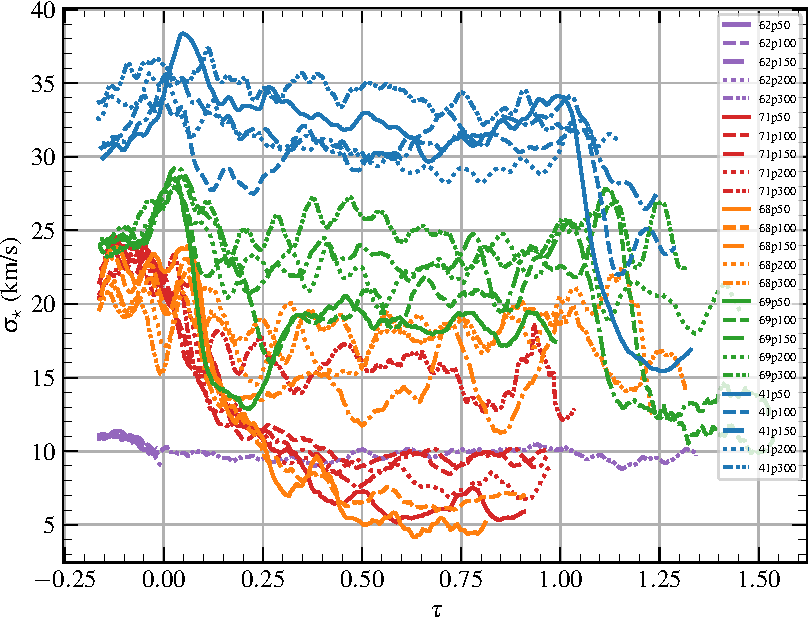
\includegraphics[width=\columnwidth]{01.0_fig_sigma_time.pdf}
\caption{Velocity dispersion evolution with time normalised with the radial period of the orbit.
}
\label{fig:sigma}
\end{figure}
For simplicity we adopted a common point of view for all the orbits, and the line-of-sight velocity dispersion is computed assuming the view laying on the orbital plane.
As tidal interactions stir the particles in the center of the galaxies, at the pericenter passages a bump in sigma can be seen.
The temporary increase in sigma can be linked to the variations of $M_h/M_\star$.
Tidal squeezing increase the velocity dispersion while subsequent mass loss can dramatically lower the sigma.
We checked the dynamical mass estimation which can be computed from the velocity dispersion in using the \citet{Wolf2010} relation:
\begin{equation*}
M^{dyn}_{est} = \dfrac{3}{G} \sigma_e^2 R_e, 
\end{equation*}
where $\sigma_e$ is the luminosity-weighted line-of-sight velocity dispersion within an effective radius $R_e$,
and $G$ the gravitational constant.



%TODO The anisotropy parameter $\beta$ is shown

% \citep{Danieli2019} Low dark matter galaxies.

\subsection{3D ellipticity}
We computed the 3D ellipticity of the stellar component of the galaxies using the Principal Components Analysis (PCA).
The first principal component $\vect w_2$ is the direction of highest elongation (largest variance of the N star particle points) computed via PCA\footnote{$\vect w_2$ is defined as the eigenvector corresponding to the largest eigenvalue of the covariance matrix $C = \frac 1 {(N-1)} AA^T$, where $A$ is the matrix of the position of the star particles centered on the barycenter of the stars.}.
% For now I took into account only the position of the star particles (which have negligible mass difference among them).

Around pericenter the main elongation direction of the ellipsoid ($\vect w_2$) is aligned with the cluster center; then it undergoes a sort of ``slingshot effect" after pericenter and it aligns with the cluster center also around apocenter before falling back in. This behaviour is shown in Figure~\ref{fig:pca}.
Around the second pericenter passage, for radial orbits, the galaxy ends up being dispersed and not anymore gravitationally bound.

In Figure~\ref{fig:pca_angle_r}, for simulation ID 69 it is shown quantitatively the relative orientation between $\vec{w}_2$ and the clustercentric direction.
Around both pericenter passages the galaxy gets aligned with the cluster center.
The maximum alignment is obtained at a delayed time depending on the radiality of the orbit.
Also, for all the orbits, the galaxy shows an aligment of an angle $<30$~deg if the orbital phase lays within a quarter of the radial period from pericenter. % ($t \in t_p \pm 0.25 T_r$).
Except for the orbit with 100 kpc pericenter, it is possible to see how at apocenter the main elongation is perpendicular to the cluster center. % For this orbit it is likely that due to a swap between 

Analogously we can compute the angle between the elongation direction and the instantaneous velocity along the orbit.
This is shown in Figure~\ref{fig:pca_angle_v}.

\begin{figure}
\centering
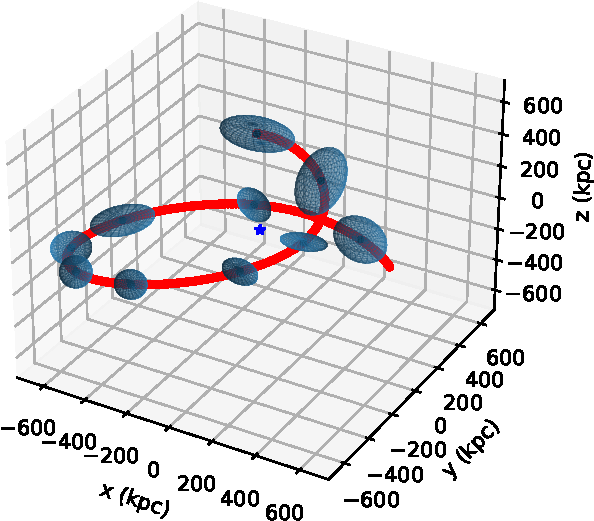
\includegraphics[width=\textwidth]{3d_qualitative_69p200.pdf}
\caption{Qualitative overview of the principal components ellipsoids for the stellar particle positions of the galaxy along the orbit. In red the orbit of the galaxy (ID 69 with pericenter of 200 kpc).}
\label{fig:pca}
\end{figure}

\begin{figure}
\centering
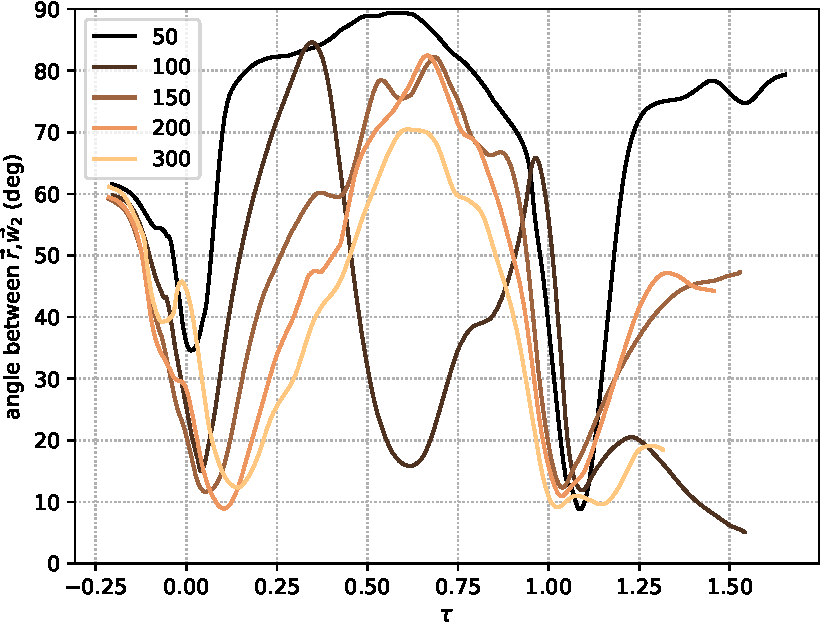
\includegraphics[width=0.8\textwidth]{69_r_angle.pdf}
\caption{Angle between the largest principal component $\vec{w}_2$ and the direction to the cluster center for simulation ID 69.}
\label{fig:pca_angle_r}
\end{figure}
\begin{figure}
\centering
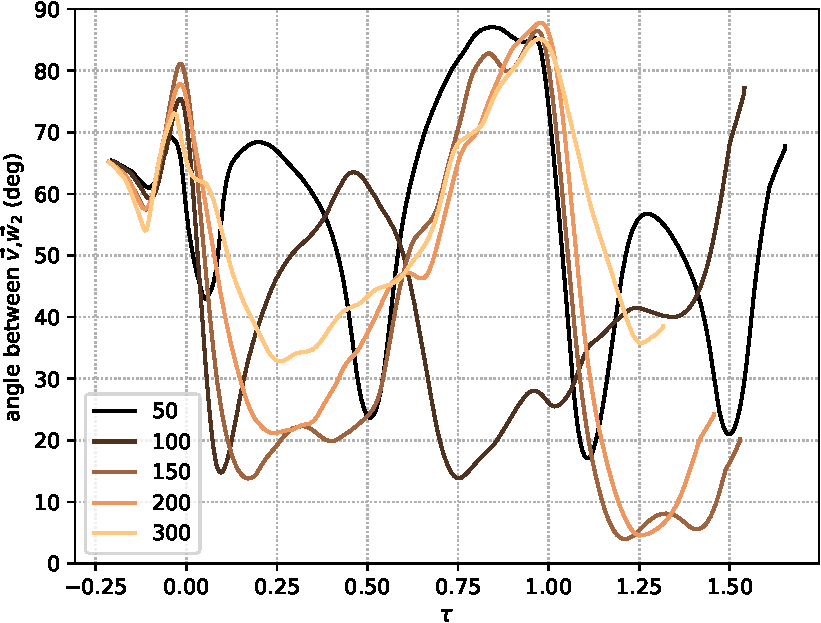
\includegraphics[width=0.8\textwidth]{69_v_angle.pdf}
\caption{Angle between the largest principal component $\vec{w}_2$ and the instantaneous velocity for simulation ID 69.}
\label{fig:pca_angle_v}
\end{figure}

\section{Star formation}
Ram pressure stripping and tidal interaction can funnel gas into the inner part of the galaxy.
In particular, tidal tails around pericenter can create grooves in the potential well which enhance the squeezing of cold gas ready to create stars.
The total content of star forming gas is shown in cyan in Figure~\ref{fig:cold_gas} alongside with the specific star formation rate.

\begin{figure}
\centering
\includegraphics[height=\textheight]{{12.6_sfr_cold_gas}.pdf}
\caption{Specific star formation rate and cold gas (T<$15000$~K) evolution on different orbits.}
\label{fig:cold_gas}
\end{figure}

In stripped tails of the jellyfish, gas is able to cool and create stars. \citet{Tonnesen2012} argue that pressure in the cluster has a primary role in regulating SF as opposed to the strength of ram pressure.
% TODO Check: Also \citet{Hausammann2019} introduce the parameter $\beta$ defined as the ratio between the ram pressure and the thermal pressure as the

% TODO compute cluster gas pressure corresponding to SFR peaks.

\subsection{Where do stars form?}
\begin{figure*}
\centering
\begin{subfigure}[t]{0.7\textwidth}
\centering
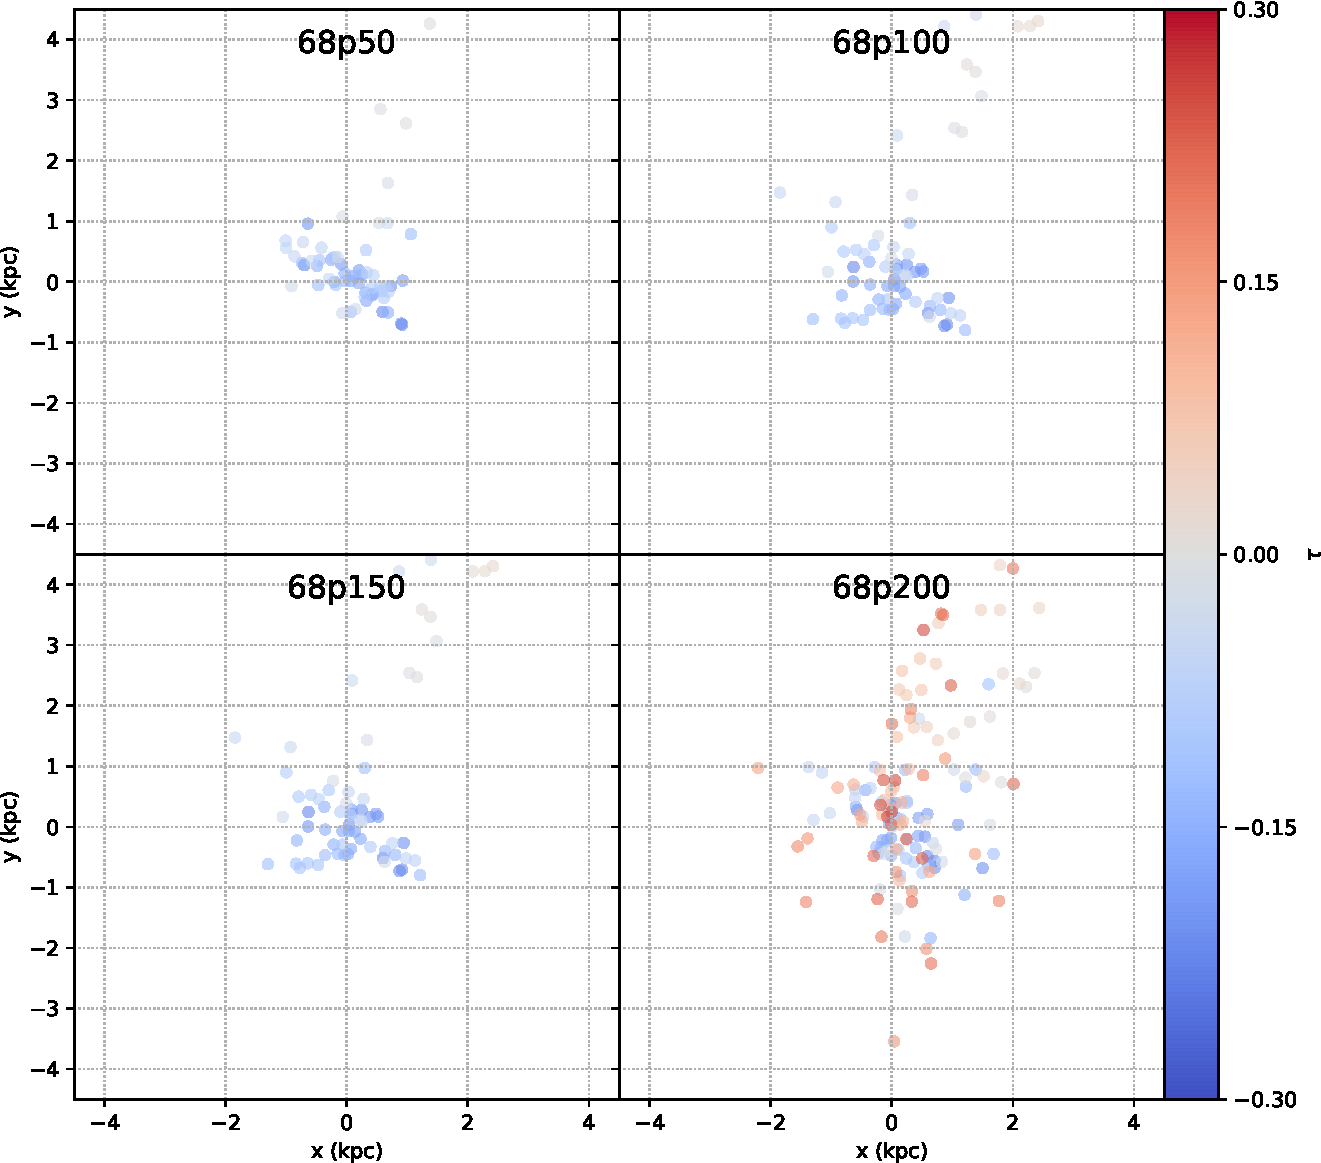
\includegraphics[width=\textwidth]{StarFormationLocation68002.pdf}
\caption{Simulation ID 68}
\end{subfigure}\\[2ex]
\begin{subfigure}[t]{0.7\textwidth}
\centering
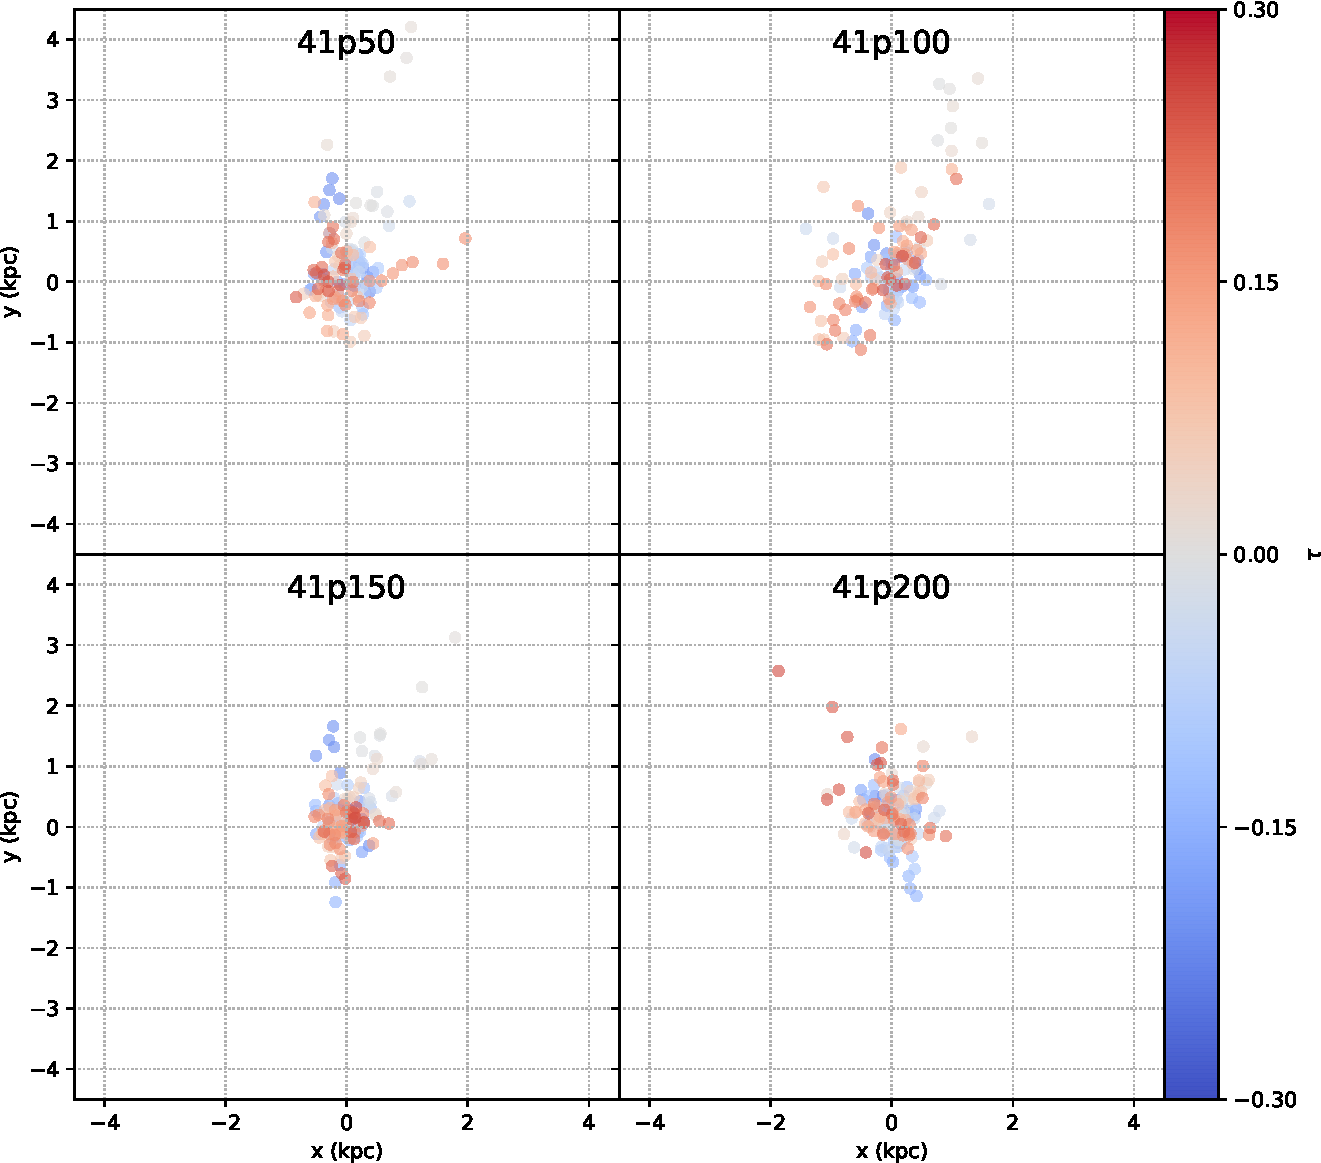
\includegraphics[width=\textwidth]{StarFormationLocation41002.pdf}
\caption{Simulation ID 41}
\end{subfigure}
\caption{Star formation location around first pericenter passage for simulation ID 68 and 41. Each subpanel corresponds to a different pericenter.
The size of the marker is proportional to the number of stars born in that time interval.
Markers are colored using the time from pericenter normalized with the radial period.
In correspondence of pericenter passage an intense star formation activity is registered in the gaseous tail.}
\label{fig:sf_location}
\end{figure*}
In Figure \ref{fig:sf_location} we show the average position of the star forming particles for each simulation snapshot.
For each simulation snapshot the number of new stars w.r.t. to the previous snapshot ($10$~Myr before) is counted and their average position in the $xy$ plane is plotted.
Galaxy is moving in the $-y$ direction (the direction of the instantaneous velocity, see \refsec{sec:MovingBox}) around pericenter.
There is a significant star formation activity in the tail (in Figure~\ref{fig:sf_location}).

An intermediate mass dwarf, ID 68, on orbit of 50 and 100 kpc is completely stripped from the reservoir of cold gas as also shown in the corresponding panel in Figure \ref{fig:cold_gas}. For this, after a burst, star formation stops.

This enforces the idea of the \emph{Jellyfish} phenomenon as a relatively short transitory phase of the galaxy. 


%% DERIVED PROPERTIES
\section{Colour Magnitude}
In Figure \ref{fig:g-r} we show the behaviour of the colour magnitude.
In particular the lightest galaxy (ID 62) does not survive the first infall yet ending its life in the early-type galaxy realm, independently of the orbit.
As shown in Figure \ref{fig:cold_gas}, the most massive one (ID 41) retains most of its cold gas except for the most radial orbit.
This is confirmed by its final location on the C-M diagram, among the early-type galaxies.
This allows for star formation to occur almost steadily and to move multiple times between early- and late-type realms.


\begin{sidewaysfigure}
\centering
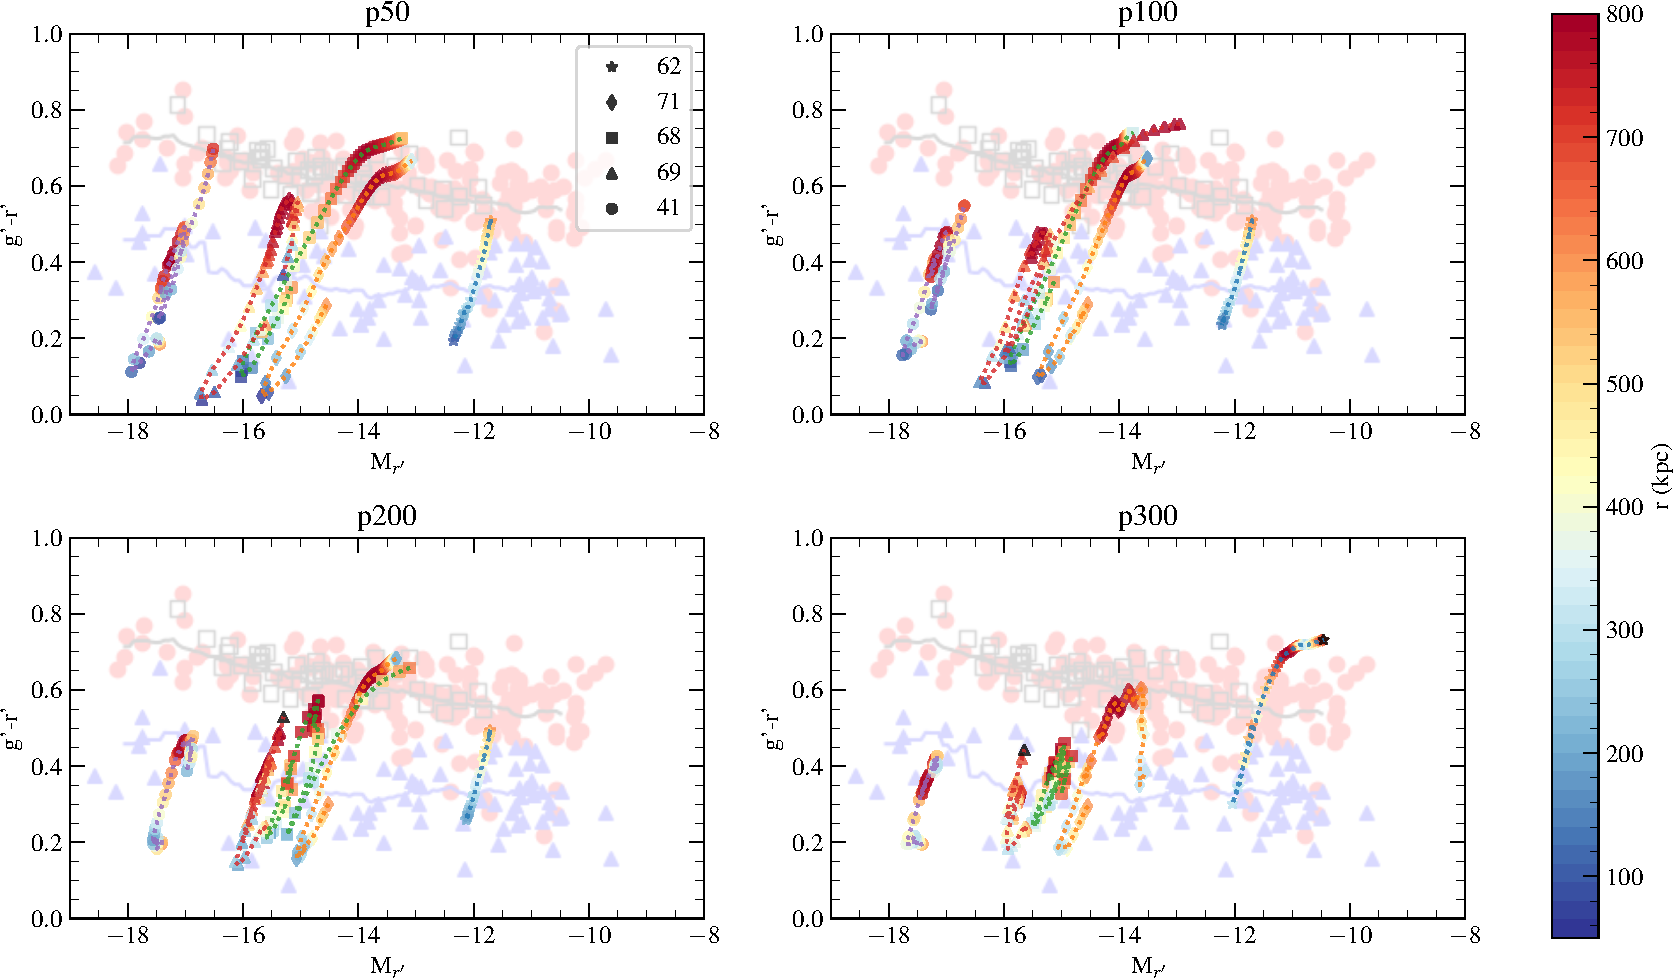
\includegraphics[width=\textwidth]{04.2_color_magnitude_Aku_g-r_rt_criterion_r.pdf}
\caption{SDSS bands colour magnitude diagram of galaxies on different orbits compared to Fornax dwarf catalogue of \citet{Venhola2019}.
% TODO ask permission for the overlay or use catalogue datapoints.
Red and blue colour for the data points in the background represent dwarf elliptical (dE) and late type galaxy respectively, classified by eye on the base of morphology. Empty squares are nucleated dE.
Data tracks of simulated galaxies are shown overlaid colour coded by the clustercentric radius.
The tracks are limited to bound galaxies (i.e. they are drawn with snapshots for which condition \eqref{eq:tidal_radius_condition} holds).
}
\label{fig:g-r}
\end{sidewaysfigure}

\section{HI size mass relation during infall}
\citet{Stevens2019} show how inevitable is the size-mass relation of neutral hydrogen, even during stripping phases.
Our simulations can be checked on the size-mass plane.
As in \citet{Verbeke2017}, we computed the \Hi{} mass by integrating the \Hi{} column density $\Sigma_{\text{\Hi}}$. The radius on the other hand is the major axis of the best fit ellipse on the $1$~\Msun{}~pc$^{-2}$ contour.

%In Figure \ref{fig:hi_size_mass} we show the behaviour of the gas of a representative dwarf.
% We see that our dwarfs stay on the \Hi{} size-mass relation.

\section{Kinematics}
To correctly compute galaxy kinematics we have to take into account the rotation of the moving box.
The details on how to recover the correct kinematics in our setup are shown in \refsec{sec:correct_kinematics}.

\subsection{Angular momentum and specific angular momentum proxy $\lambda_R$}
We compute the specific stellar angular momentum proxy $\lambda_R$ starting from SPH luminosity-weighted velocity and velocity dispersion maps as defined in \citet{Emsellem2007}: %\citet{Toloba2015}
\begin{equation}
    \lambda_R = \dfrac{\sum_i F_i R_i |V_i|}{\sum_i F_i R_i \sqrt{V_i^2 + \sigma_i^2}}
\end{equation}
with $i$ the pixel index, $F_i$ its flux and $R_i$ the distance of the pixel from the galaxy center.
This parameter has been introduced to better captures the spatial information included in the kinematic maps.
As opposed to the classical $\frac{v}{\sigma}$ indicator, $\lambda_R$ has been designed to distinguish between galaxies with kinematically decoupled components (KDC).

An example of the maps from which $\lambda_R$ is computed are shown in Figure~\ref{fig:maps_lambda_r}.
The $V_{LOS}$ and $\sigma$ map are computed with SPH interpolation, using the luminosity in $v$-band to weight the contribution of particles along the line of sight.
Some authors \citep[e.g.][]{Schulze2018,Pillepich2019} use non-weighted quantities taken directly from the particles to compare simulations and observation, even if what is observed are luminosity-weighted quantities.
This approach makes the comparison with observations more difficult since all the information that we get is luminosity weighted \citep{Walo-Martin2020}.

\begin{figure}
\centering
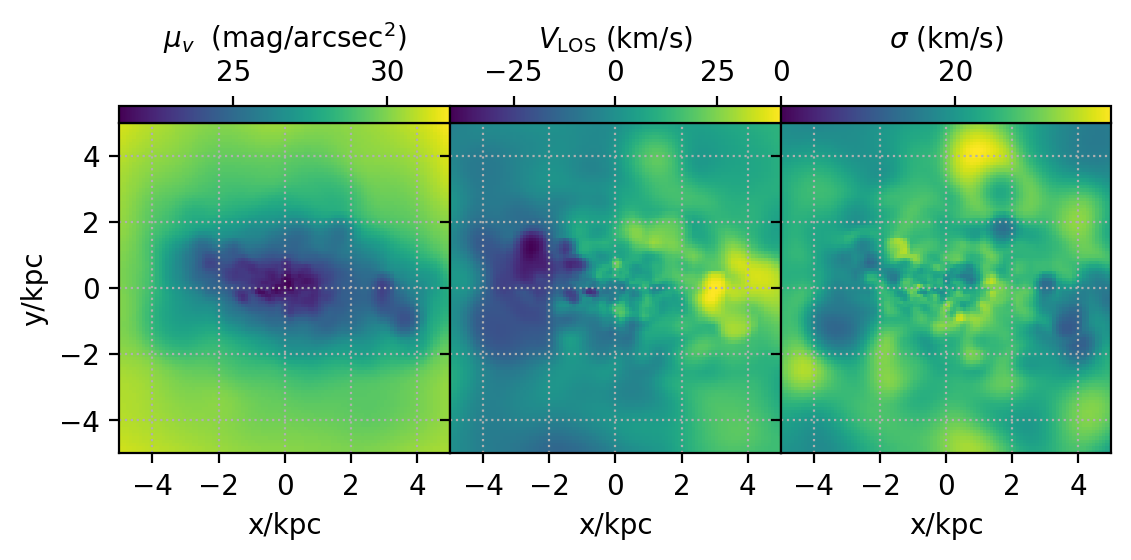
\includegraphics[width=\textwidth]{mu_v_sigma_69p150s60_sideon.png}
\caption{$\mu_v$ surface brightness map and SPH v-band luminosity weighted maps of line of sight velocity and velocity dispersion $\sigma$ for a snapshot of the simulation ID 69 around first pericenter passage.
The galaxy is projected edge-on, with the angular momentum vector lying on the $xy$ plane.}
\label{fig:maps_lambda_r}
\end{figure}

It is possible to compute the radial profile of $\lambda_R(r)$, as in Figure~\ref{fig:lambda_r_profile}.

The value $\lambda_R(R_e) = \lambda_{R_e}$ is used to distinguish between fast and slow rotators.
\citet{Emsellem2007} defines galaxies with $\lambda_R < 0.1$ as ``slow rotators'' whereas the one with $\lambda_R>0.1$ as ``fast rotators''.
As shown in figure \ref{fig:lambda_r_profile}, galaxies while falling into the cluster, evolve from being classified as having a fast rotators profile to slow rotator \citep[cf.][]{Emsellem2011}.

% Obviously this distinction depends on the real inclination of the galaxy, as it appears in the sky. % TODO possible to include inclination in a plot?

It has been shown in the \textsc{SMAKCED} survey of 39 early-type galaxies in the Virgo cluster \citep{Toloba2014, Toloba2015} that the so classified fast-rotator galaxies in the outer region of the cluster rotate faster than the fast rotators in the center of the cluster.
The specific angular momentum $\lambda_R$ is correlated with clustercentric distance.
It is indeed hypothesized, that after pericenter passages and a long time in the cluster, galaxies are heated up and transformed into slow rotating dEs.
This scenario is confirmed by our simulations where dwarf irregulars are converted to early-type galaxies and their kinematics is transformed into the one of slow rotators.


\begin{figure}
\centering
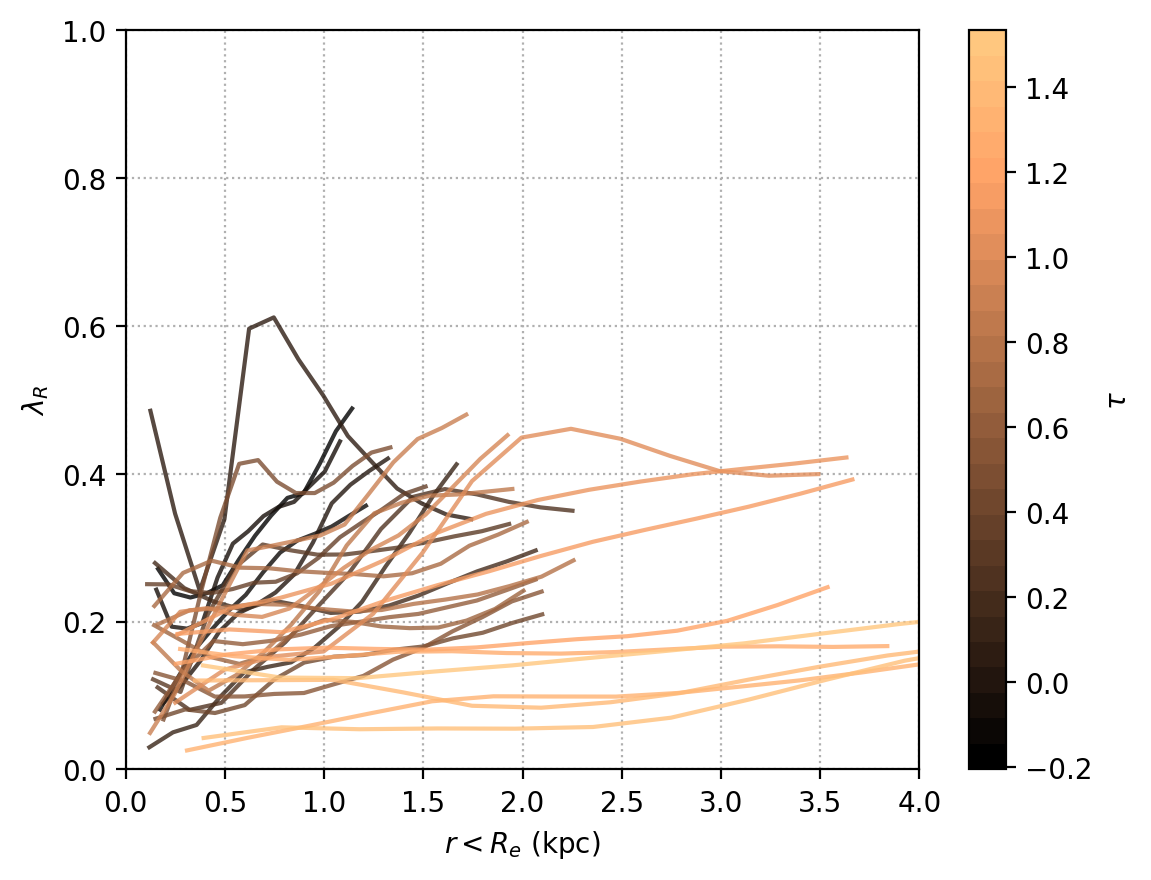
\includegraphics[width=\textwidth]{lambda_r_profile_69p150_each20_up_to_r_e.png}
\caption{$\lambda_R$ profiles for ID 69 on a 150 kpc orbit color coded with time normalized by radial period. The $\lambda_R$ profile is show up to the corresponding $R_e$.}
\label{fig:lambda_r_profile}
\end{figure}



\begin{figure}
\centering
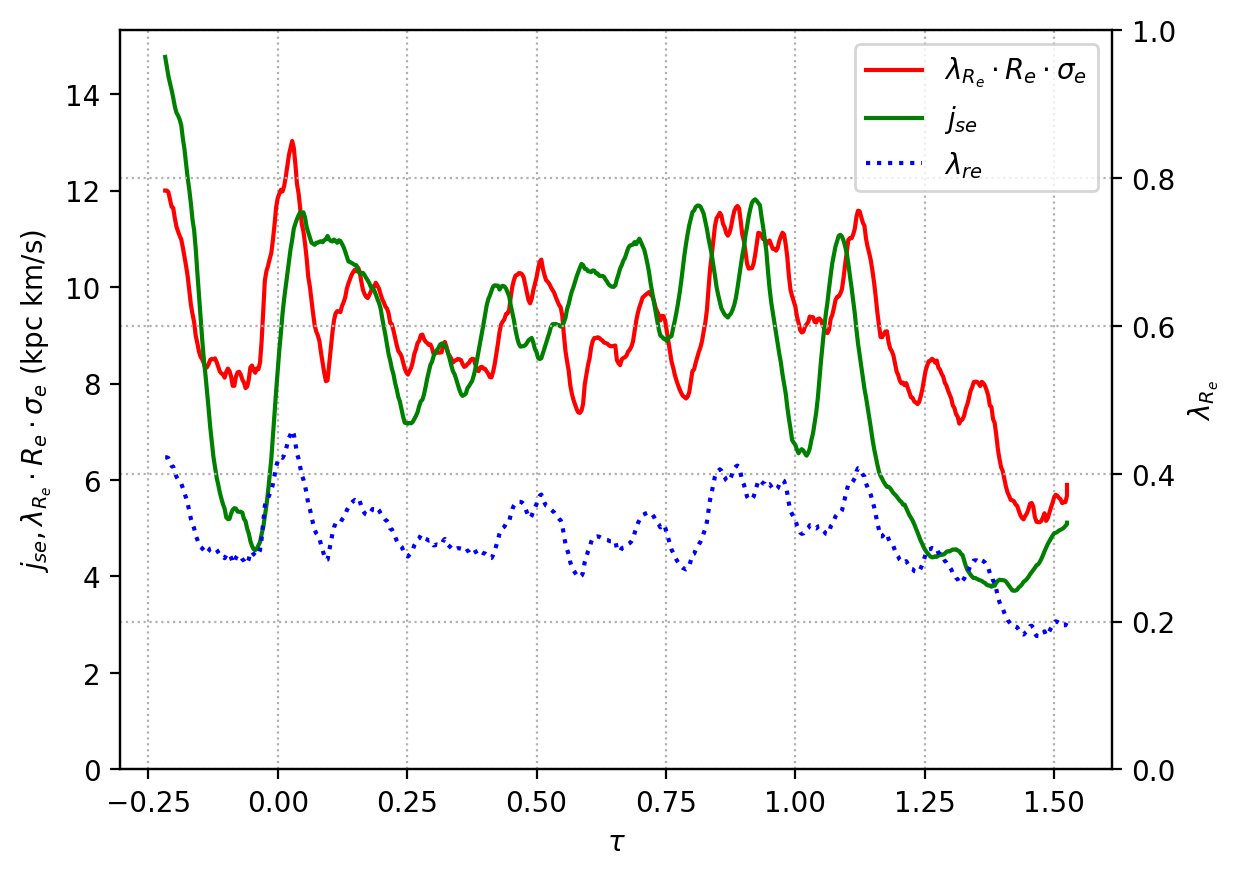
\includegraphics[width=\textwidth]{lambda_r_j_s_69p150r100.png}
\caption{Comparison between specific angular momentum and $\lambda_R$ at the effective radius for ID 69 on a 150 kpc orbit.}
\label{fig:lambda_r_j_s}
\end{figure}


% A typical evolution of $\lambda_R$ through time is shown in Figure~\ref{fig:lambda_R}.
\begin{figure}
\centering
\includegraphics[height=\textheight]{{02.1_lambda_r_vs_js}.pdf}
\caption{Stellar specific angular momentum $\lambda_R$ and specific angular momentum of star particles $j_s$ for the simulation ID 69 on multiple orbits.}
\label{fig:lambda_r_j_s}
\end{figure}

% TODO The relative increase of $\lambda_R$ at first pericenter passage is shown for each orbit and mass in figure \ref{fig:ssam_relative}.
% Around pericenter passages an increase of $\lambda_R$ by a factor of $\approx 2$ is observed.

% \citep{Bidaran2020}

\subsection{Relation with physical angular momentum}
We compute the specific angular momentum ($j_s = J_s/M_\star$ where $J_s$ is the total angular momentum and $M_\star$ the stellar mass of the galaxy) of star particles within 10~kpc from the densest stellar region (center of the galaxy).
We compare this specific angular momentum with $\lambda_R$ in Figure \ref{fig:lambda_r_j_s}.
We notice that for example in simulation ID 69, $\lambda_R$ behaviour is very oscillating, quite prone to bursty star formation which can abruptly affect its value.
In our measurements, $\lambda_R$ fails to distinguish pericenter passages unequivocally.
For these reasons in the case of dwarf irregulars it is not a good indicator of the real rotation of the galaxy.
% TODO 41 69 71
% 
% \begin{figure}
% \centering
% 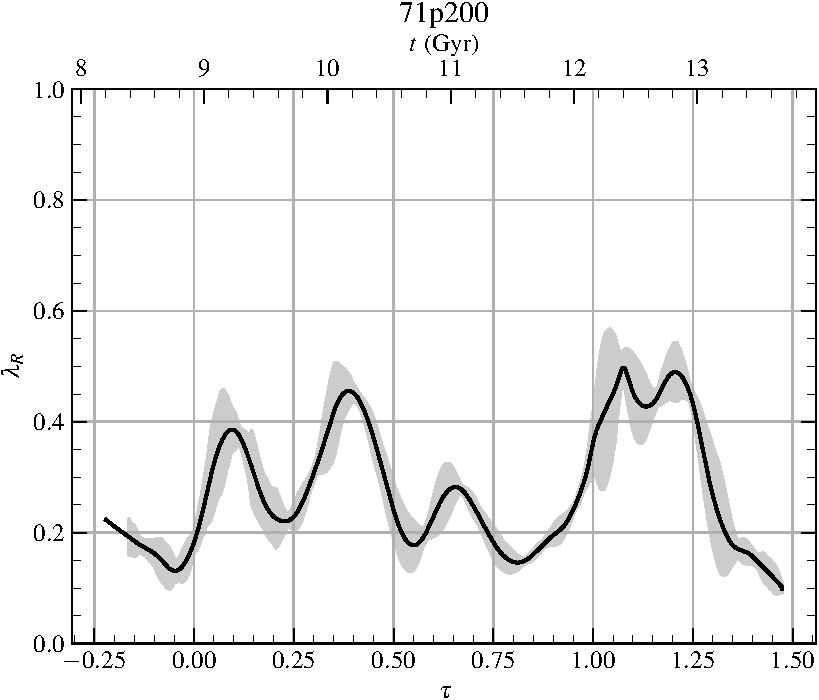
\includegraphics[width=.8\columnwidth]{03.0_fig_lambda_r_time.pdf}
% \caption{Specific stellar angular momentum for galaxy ID 71 on a $200$~kpc pericenter orbit.}
% \label{fig:lambda_R}
% \end{figure}

\section{Conclusion}


% \subsection{Magnitude conversion}
% \pynbody{} can be programmed to compute luminosities of stellar particles using 
% The built in libraries are from Marico... Padova... %TODO
% To obtain SDSS bands we ued conversion formulas from here, after having computed the magnitudes in Johnson bands.
% 
% In particular:



% !TEX root = thesis.tex

{
\cleardoublepage% Move to first page of new chapter
\let\cleardoublepage\relax% Don't allow page break
\noindent \small{Based on: \emph{A tale of two tails: insights from simulations into the formation of the peculiar dwarf galaxy NGC~1427A}, Mastropietro~M., De Rijcke~S., Peletier~R.F. \citet{Mastropietro2020}
}
\chapter[A tale of two tails: on the formation of NGC~1427A]{Insights from simulations into the formation of the peculiar dwarf galaxy NGC~1427A}
\label{ch:ngc1427a}
}

\abstract{
We present a scenario for the formation and the morphology of the arrow-shaped dwarf irregular galaxy NGC~1427A in the Fornax Cluster.
This galaxy shows intriguing stellar and gaseous tails pointing in different directions for which alternative but not conclusive formation scenarios have been proposed in the literature.
We performed $N$-body/SPH simulations of dwarf galaxies falling into a model of the Fornax cluster, exhibiting a jellyfish-like appearance while undergoing ram-pressure stripping.
We noted that some of our models show interesting tail morphologies similar to that of NGC~1427A.
In this way, the peculiar NGC~1427A structure can be studied using models whose stellar and neutral gas photometry and kinematics are in good agreement with the observed ones, without the need of invoking an interaction with a nearby galaxy.
Thanks to the tails, we can identify the requirements for a galaxy to expose such a structure and assess the possible position and velocity of the galaxy in the cluster.
This puts constraints on the orbit of the galaxy, its position in the cluster and the time since its pericenter passage.
From the statistics of identified snapshots following our modelling, we found that the most likely position of the galaxy is around $200$~kpc in front of the cluster center, travelling towards the cluster with a velocity angle with respect to the line-of-sight direction of around $50$~deg.
This analysis can be useful in future observations of similar galaxies in clusters to characterise their position and velocity in the cluster and their formation.
}


\section{Introduction} \label{sec:intro}

\begin{figure*}
\centering
\includegraphics[width=\textwidth]{NGC1427A-crop.png}
\caption{False-colour image of NGC 1427A, based on HST Advanced Camera for Surveys (ACS) archival data (Proposal ID: 9689; PI: M. Gregg).
The following colour bands were used: blue=475W; green=775W; red=625W+660N (stellar emission was subtracted from the 660N image using a scaled 775W image).
This colour scheme makes the H$\alpha$ emission stand out in red. An asinh stretch was applied to bring out also the faint details.
The inset zooms in on the Northern Clump, showing it to be composed of two loose stellar clusters with embedded \Hii{} emission.
The Northern Clump also appears to be connected to the north-west rim of NGC 1427A's main body via a tenuous stream of stars.
The directions of the \Hi{} tail and towards the Fornax Cluster center are indicated with arrows.
The dotted ellipse is the same as in Figures 1 and 2 of \citet{Lee-Waddell2018} and indicates the shape and direction of the faint outskirts of the galaxy, which are quite distinct from the system's inner, brighter parts.
}
\label{fig:NGC1427A}
\end{figure*}
The evolution of galaxies in dense environments has been shown to be markedly different from that of more isolated galaxies, with mass being a prominent factor in determining how profoundly environmental influences affect a galaxy \citep{Boselli2006, Grossi2018a}. 
The well-known morphology-density relation, according to which early-type galaxies are mostly found in high-density environments \citep{Dressler1980, Dressler1997}, is especially pronounced for low-mass systems, such as dwarf galaxies \citep{McConnachie2012}.
Indeed, while actively star-forming late-type dwarf galaxies are found almost exclusively in low-density environments, truly isolated quiescent early-type dwarf galaxies, on the contrary, are exceedingly rare \citep{Binggeli1990, Karachentseva2010, Geha2012}.

An effective way of shutting down the star formation in a galaxy is to rob it of the raw material for building stars:~gas. 
When a galaxy enters on an orbit in a galaxy cluster or group, it is subjected to the tidal forces of the cluster potential and of its galaxies. 
Its interstellar medium experiences the ram pressure \citep{GunnGott1972}, basically a supersonic ``headwind", exerted by the intracluster medium.
Ram pressure is a well known phenomenon and many studies have been devoted to simulating its effects on galaxies \citep[e.g.:][]{Mori2000, Mayer2006, Roediger2008, Roediger2015, Steinhauser2016, Yun2018, Steyrleithner2020}.
If the ram pressure is sufficiently vigorous, the galaxy's diffuse interstellar medium can be pushed out of its gravitational well, forming a tail of escaping \Hi{} gas in the galaxy's wake.
The much more clumpy molecular gas is not as easily removed by the ram pressure and remains behind while being consumed by star formation \citep{Abramson2014, Lee2017, Wang2020}. 
Inside the tail, gas can cool and form knotty condensations, leading to a complex stellar system, with a head consisting of the galaxy's stellar body (and what remains of its gas) and a tail of twisting swirls of stripped gas, beaded with knots of star formation.

The term \emph{jellyfish galaxies} \citep{Ebeling2013} neatly fits this description and hence they are prime candidates for interpreting the transformation processes acting on galaxies in cluster and group environments.
Jellyfish galaxies exhibit tentacles of material that appear to be stripped from the galaxy body \citep{Poggianti2017a, Poggianti2019b, Ramatsoku2020}.
The term applies to galaxies with star formation activity within the stripped gas tails.
Signatures of the newly born stars within those gaseous tails are easily found in UV or blue images \citep{Cortese2007,Smith2010a,Poggianti2017a}. In particular, as will be explored more in detail in Chapter \ref{ch:sim_results}, star formation flickers on and off inside the gaseous tails of simulated ram-pressure stripped dwarf galaxies as gas clumps condense and disperse again. This gives the label ``jellyfish galaxy" a transient and possibly recurrent quality.

The distorted optical appearance and gaseous tails and overall jellyfish-like morphology --~barring currently active star formation in the gas tails~-- of NGC 1427A (Figure \ref{fig:NGC1427A}) seems to be straightforwardly and satisfactorily explained by ram-pressure stripping in conjunction with cluster tidal forces.
To correctly interpret the available data, it is of prime importance to be able to reliably identify the dominant transformation process for this galaxy.
With this goal in mind, we compare recent \Hi{} and optical data of NGC~1427A with a suite of dwarf galaxy simulations, set in a Fornax Cluster environment.

In the next section, we give a short overview of the observed properties of NGC 1427A and focus on those that are considered most relevant for elucidating its origin and evolution. In Section \ref{sec:simulations}, we present the numerical details of our simulations. The methodology behind the comparison of these simulations with the observations is discussed in Section \ref{sec:results}. We conclude with a discussion of the main results in Section \ref{sec:discussion}.


\section{Observed properties of NGC~1427A} \label{sec:observations}
\begin{figure*}
\centering
\begin{subfigure}[b]{0.49\textwidth}
  \centering
  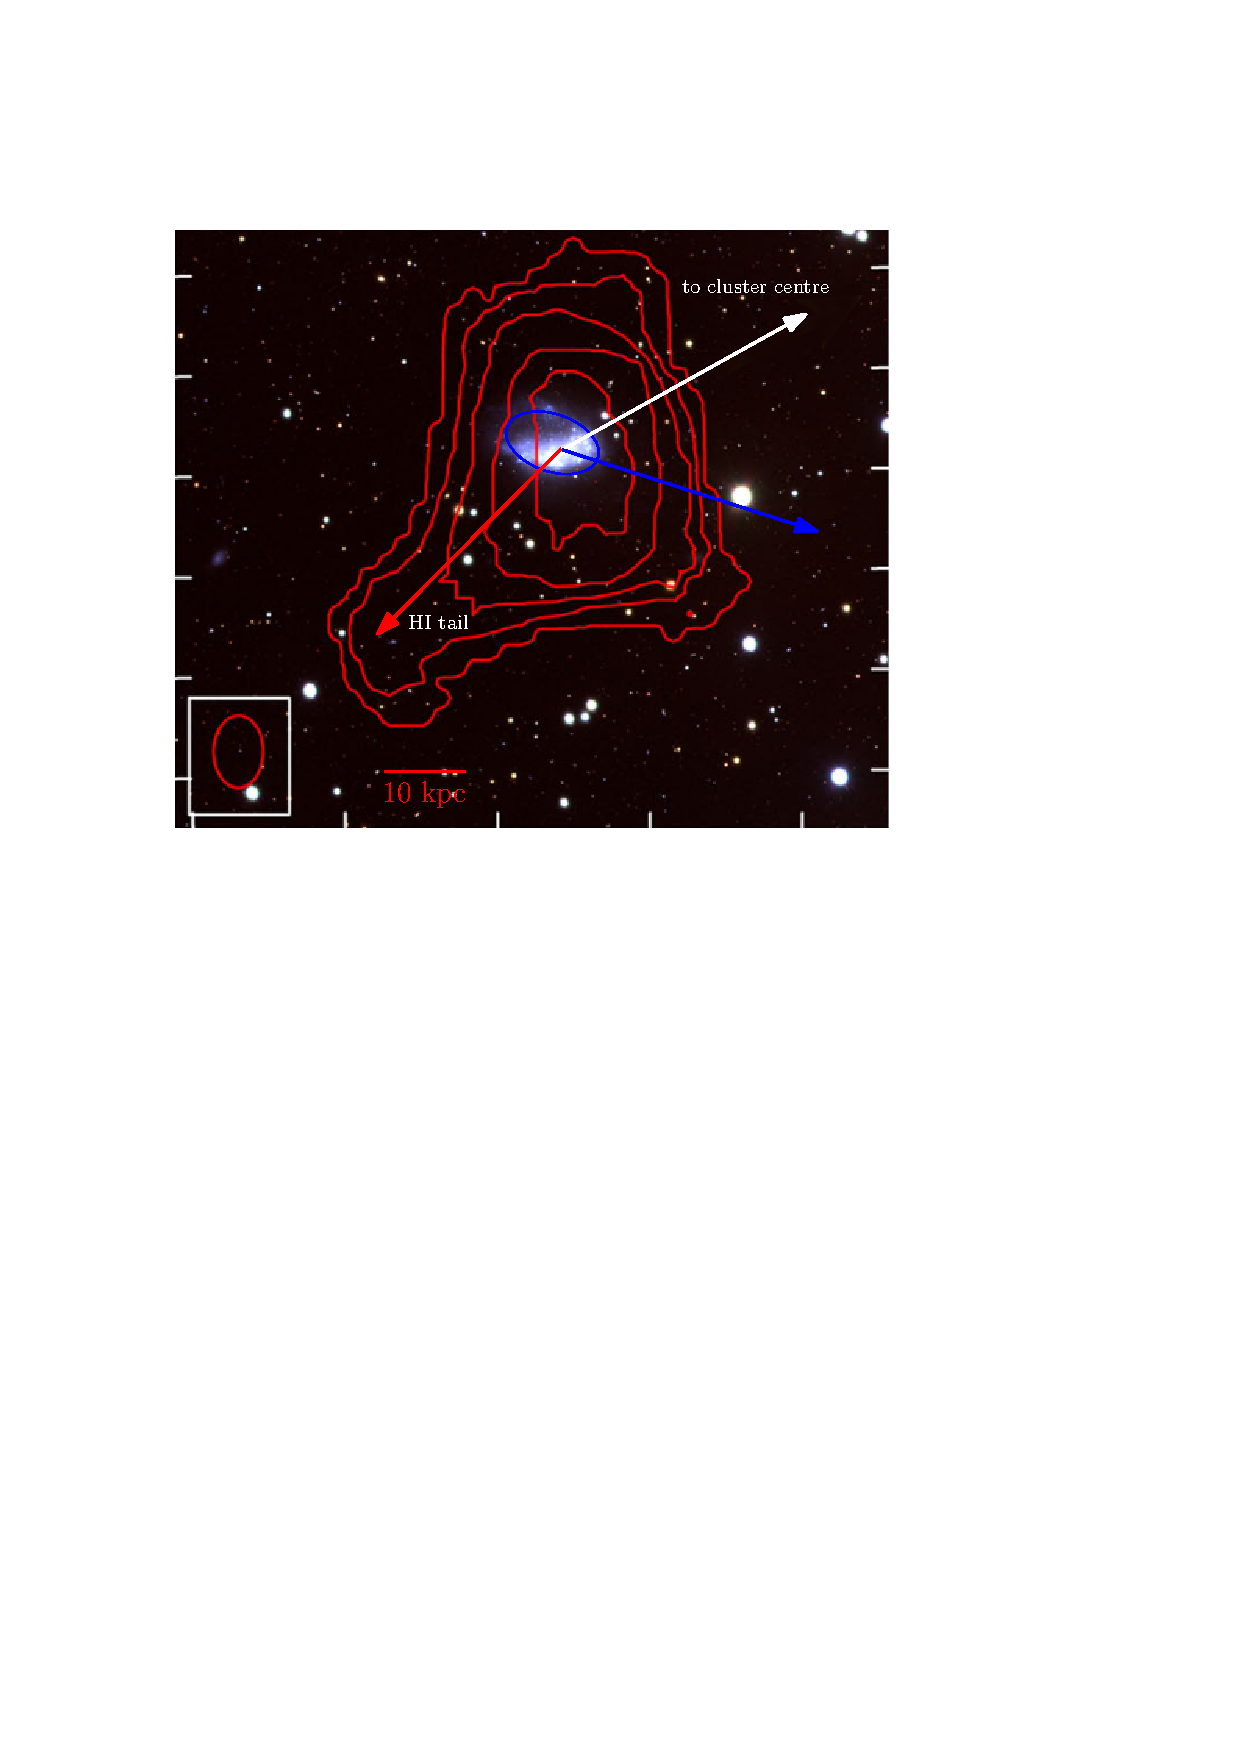
\includegraphics[width=\textwidth]{NGC_LIKE/ngc_location_scale.pdf}\\[3ex]
  \caption{}
  \label{fig:hi_contours}
\end{subfigure}
% \hfill
\begin{subfigure}[b]{0.49\textwidth}
  \centering
  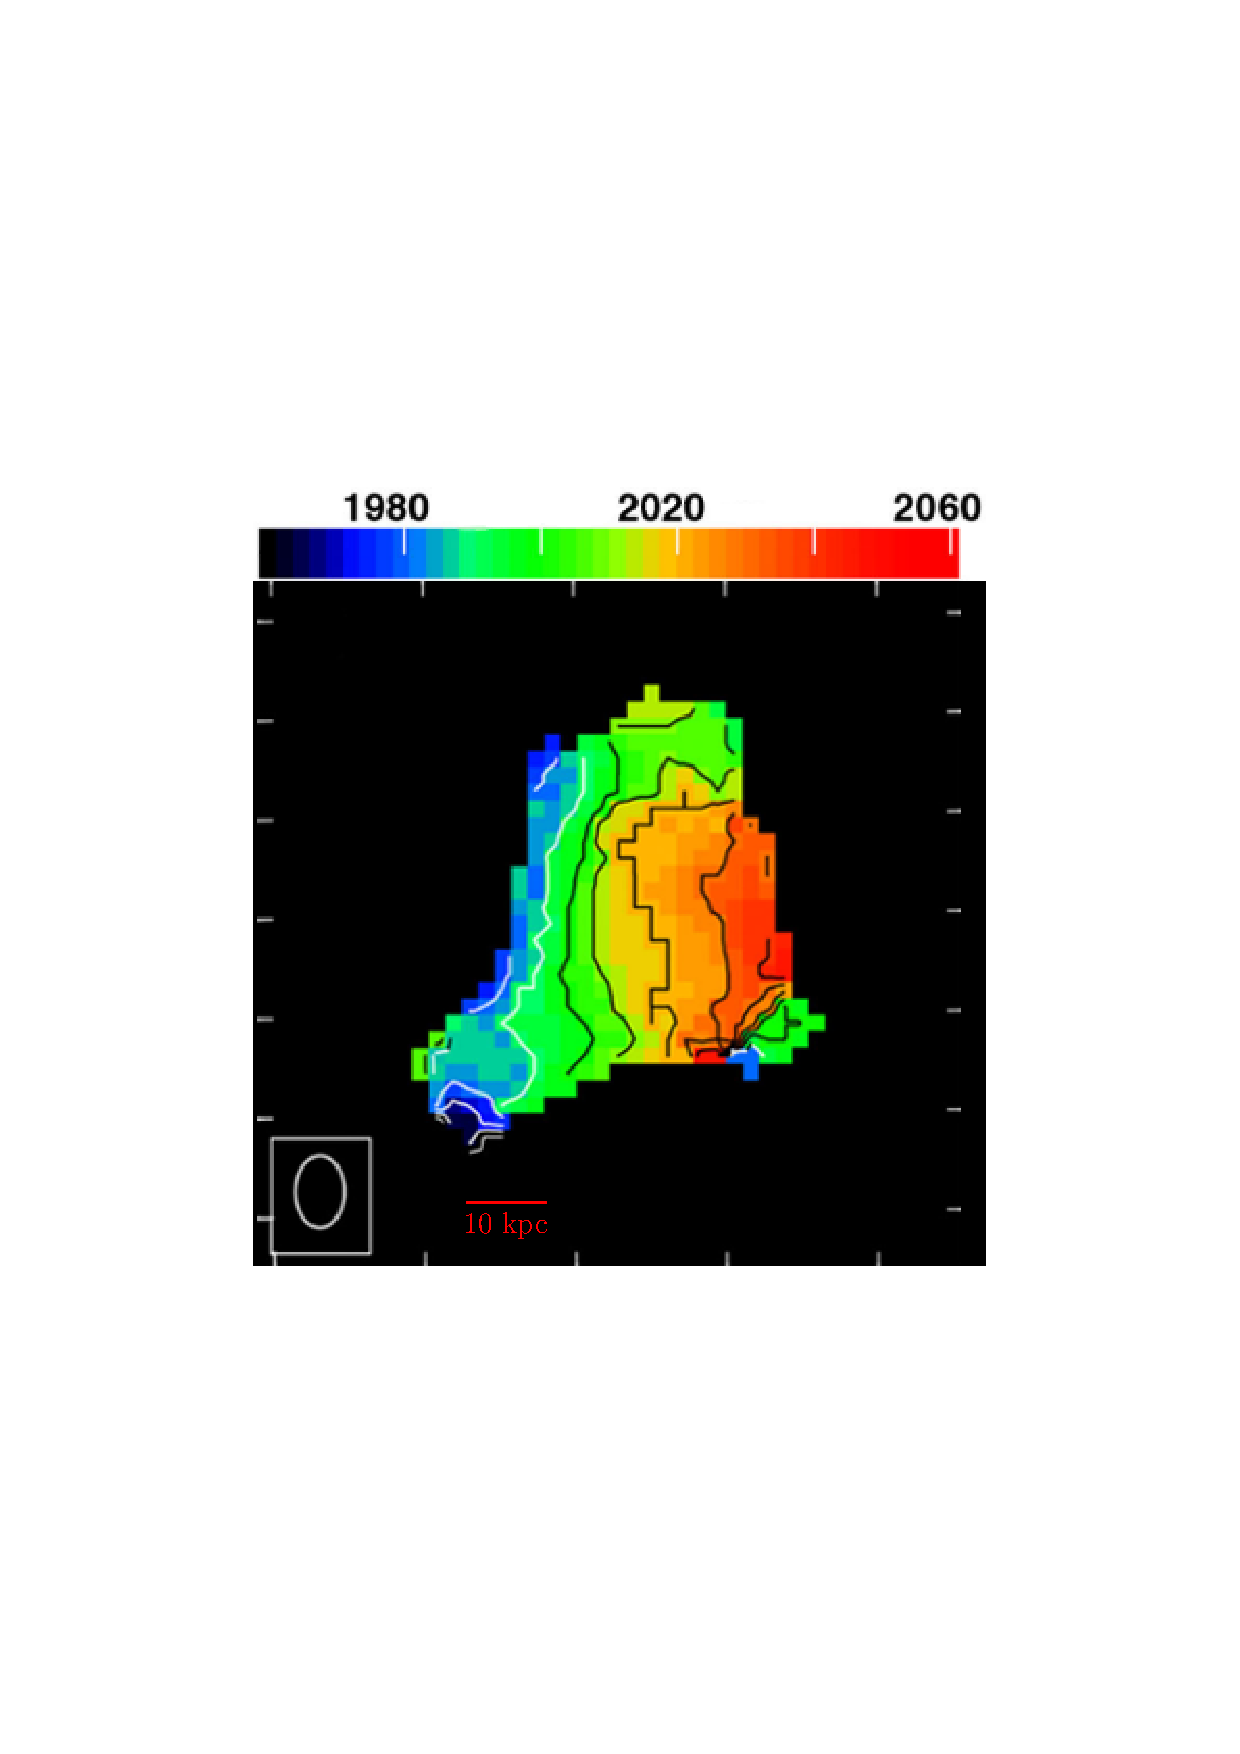
\includegraphics[width=0.9\textwidth]{NGC_LIKE/kin_scale.pdf}\\[3ex]
  \caption{}
  \label{fig:hi_kin}
\end{subfigure}
\begin{subfigure}[b]{0.6\textwidth}
  \centering
  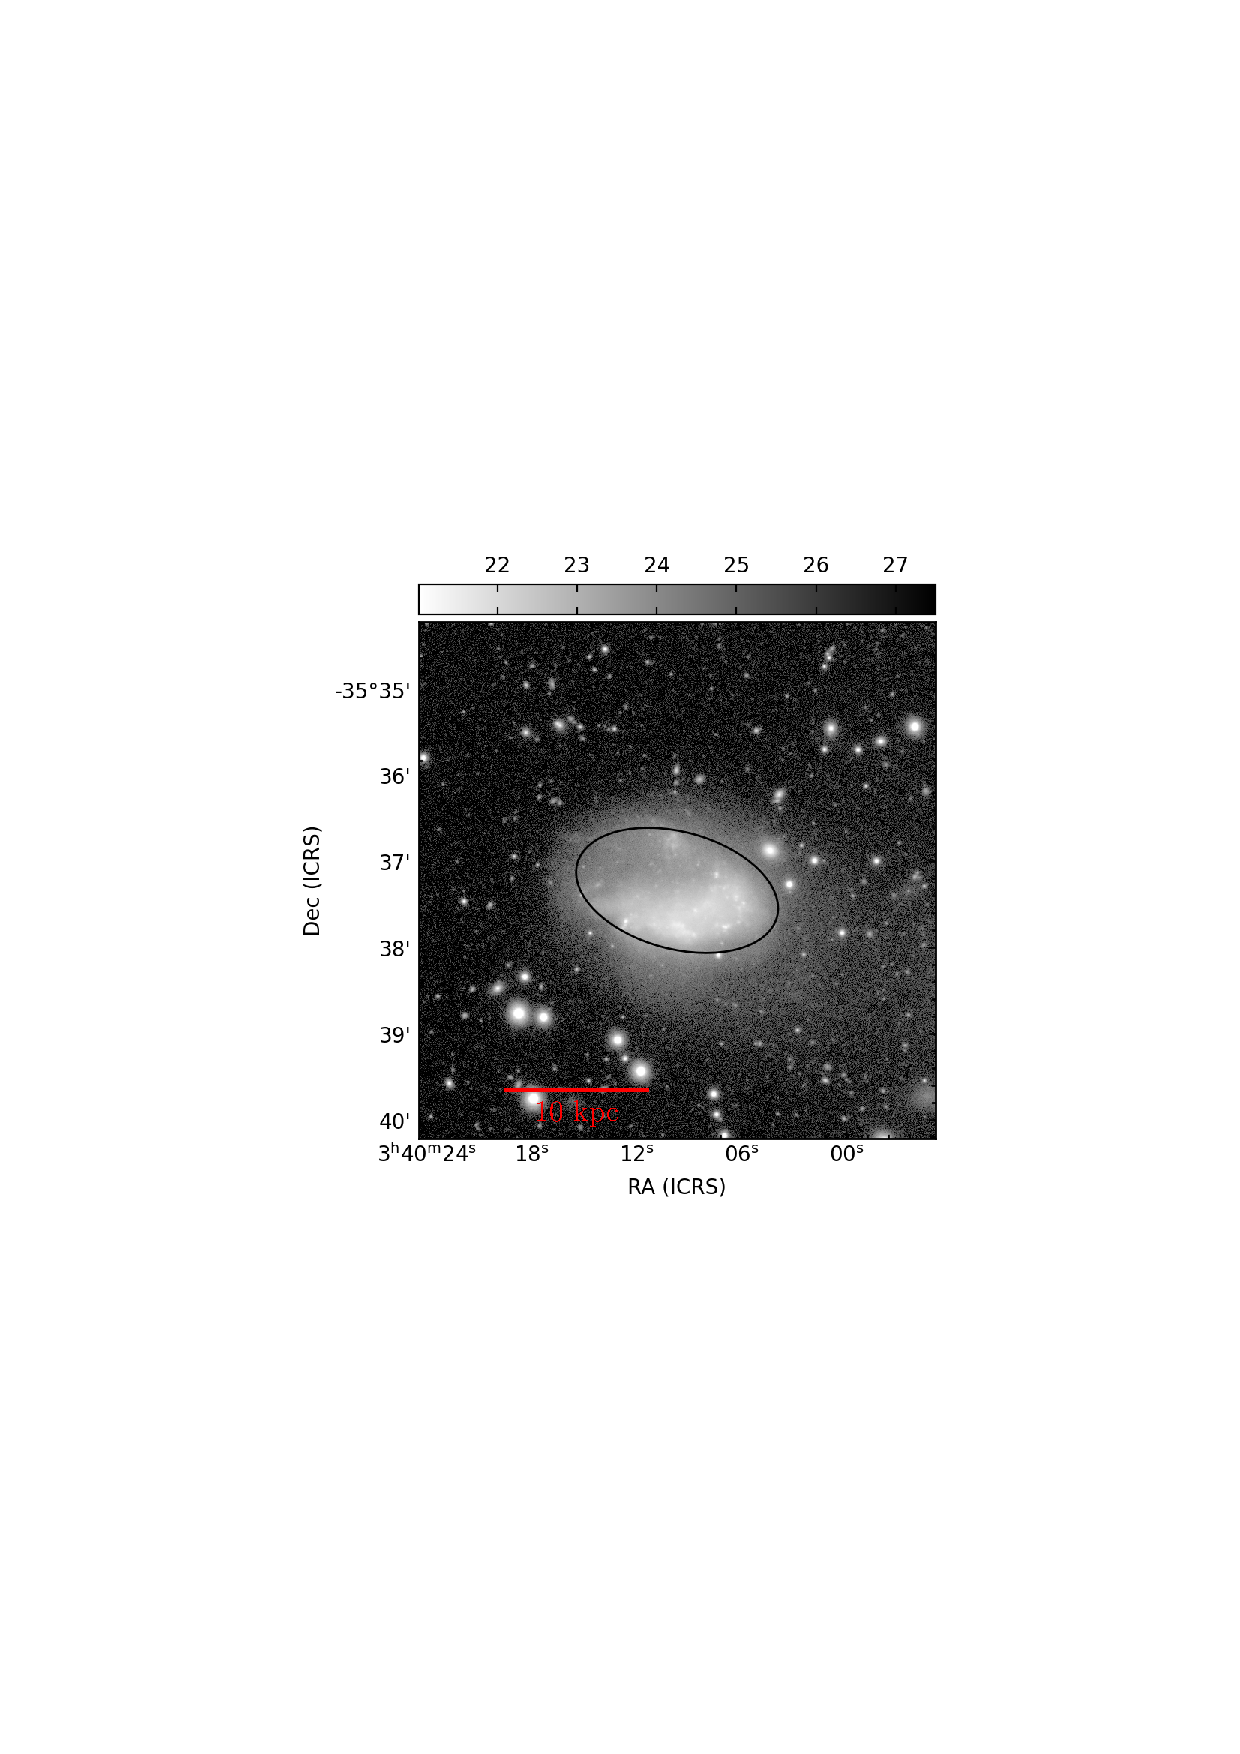
\includegraphics[width=\textwidth]{NGC_LIKE/ngc_tide_scale.pdf}%\\[3ex]
  \caption{}
  \label{fig:r_band}
\end{subfigure}
% \hfill
\caption{
Images of NGC~1427A from \citet{Lee-Waddell2018} for illustrative purposes:~(a) VST image with overplotted in red contours of constant \Hi{} column density at levels $(0.5, 1, 2, 5, 10) \times 10^{20}$~amu~cm$^{-2}$;
(b) gas kinematics (recessional velocity in km/s)
(c) $r'$-band image (in mag/arcsec$^2$).
A length scale at the assumed cluster distance is indicated in red.}
\label{fig:NGC_OBSERVATIONS}
\end{figure*}
NGC 1427A is a gas-rich dwarf irregular galaxy in the Fornax Cluster.
Recessional velocity measurements indicate that NGC~1427A is moving with a line-of-sight velocity of around 2028 km/s \citep{Bureau1996, Schroder2001}.
Accordingly, if we assume NGC~1399 to be the cluster center, NGC~1427A travels away from us at a projected speed of around 700~km/s w.r.t. the cluster center. NGC 1427A has a projected distance of 137 kpc from NGC1399\footnote{The angular separation is 1373$\arcsec$ = 137~kpc, throughout the paper, we assume a fiducial distance of the cluster center of 20~Mpc.}.

A false-colour HST image of the galaxy is shown in Figure~\ref{fig:NGC1427A}.
The inset of Figure \ref{fig:NGC1427A} zooms in on the Northern Clump, showing it to be composed of two loose stellar clusters with embedded \Hii{} regions. The Northern Clump also appears to be connected to the north-west rim of NGC~1427A's main body via a tenuous stream of stars. The directions of the \Hi{} tail and towards the Fornax Cluster center are indicated with arrows. The dotted ellipse is the same as in Figures 1 and 2 of \citet{Lee-Waddell2018} and indicates the shape and direction of the faint outskirts of the galaxy. We interpret these low-surface-brightness stellar features, which point towards the north-east and south-west (effectively captured by the ellipses in Fig. \ref{fig:NGC1427A} and \ref{fig:r_band}), are quite distinct from the much brighter inner regions of the galaxy's main body, as tidal features. The Northern Clump, which we discuss in detail in section \ref{NC1427A}, may be associated with these tidal features.

\citet{Chaname2000} presents a lower limit for the dynamical mass of NGC 1427A using a rigid-body rotation model: $M_{\mathrm{dyn}}~>~(9\pm 3)\times 10^9 M_\odot$. Following the calibrated empirical relation of \citet{Taylor2011}, the stellar mass estimated by \citet{Lee-Waddell2018} is $M_{\star} \approx 10^9 M_\odot$ while its total \Hi{} mass is determined to be $M_{\mathrm HI} = (2.1 \pm 0.2) \times 10^9 M_\odot$.
The galaxy has a conspicuous \Hi{} tail, containing about $10$ per cent of all \Hi{} gas in NGC~1427A, pointing towards the south-east as well as stellar tidal extensions along a north-east to south-west axis. In other words:~the gaseous and stellar extensions are almost perpendicular to each other. NGC~1427A was not detected in CO emission, providing an upper limit on its molecular gas mass of the order of $M_{\mathrm H_{2}}~\sim 10^8$~M$_\odot$ \citep{Zabel2019}. These authors report the detection of a single 3~mm continuum source without an optical counterpart but its nature remains unclear.
A distinct young stellar clump is visible in the northern rim of the galaxy. On high-resolution images, this clump, the rim, as well as the galaxy's main stellar body are resolved into many individual OB associations and clusters, some with accompanying H$\alpha$-emission \citep{Hilker1997, Sivanandam2014}. Clearly, star formation proceeds in many dispersed small bursts.

Various hypotheses regarding the evolution of NGC 1427A, and especially its extraordinary configuration of tails, have been proposed. These include recent interactions with other nearby galaxies \citep{Cellone1997}, a merger with an object that now forms the northern stellar clump \citep{Lee-Waddell2018}, the tidal interaction with the cluster potential, and ram-pressure stripping of its gas by the cluster hot gas halo \citep{Chaname2000, Mora2015}.
%This galaxy has been described by \citet{Laustesen1987} with this expression \emph{"It contains a large number of gaseous and luminous clusters, which partially form a ring towards the western edge of the galaxy”}. \citep{Cellone1997}
%What \sven{is especially striking} regarding NGC 1427A is the relative direction of its twin stellar and gaseous tails\sven{:~they are almost perpendicular to each other}.
% Various hypothesis on the formation scenarios have been proposed \cite{Hilker1997, Cellone1997, Chaname2000, Mora2015, Lee-Waddell2018}:
% tidal interactions with other nearby galaxies, tidal interaction with the cluster potential and ram pressure stripping of its gas by the cluster hot gas halo.

To try and identify the environmental processes acting on NGC~1427A, we first selected those properties of this dwarf galaxy that were most likely to be indicative of those processes and not of internal effects. Those are:
\begin{enumerate}
    \item the direction towards the Fornax cluster centrum, 
    \item the direction of the axis of the stellar tidal extension,
    \item the direction of the \Hi{} tail.
\end{enumerate}
These parameters are most tightly linked with NGC~1427A's orbit through the Fornax Cluster and are expected to be relatively insensitive to the accidents and vagaries of its evolution before its acquisition by the cluster. 

Thus, our analysis differs from that of \citet{Lee-Waddell2018} where the ram-pressure hypothesis is discussed based on stellar colour and galaxy morphology information.
Their new data indeed rule out a ram pressure origin for the optical appearance of the galaxy, but they leave open the question whether ram pressure may have played a role in the formation of the \Hi{} tail.

% We carried out a morphological search throughout our suite of simulations to isolate snapshots with the above properties respecting.% which can be useful to characterise the effects leading to such peculiar morphology.
% We found that the main effects generating peculiar morphology are indeed the combination of galaxy rotation, ram pressure and tidal interaction close to the cluster center.
% % It's clear also (see Figure \ref{fig:3dview}) that gaseous and stellar components react differently to the main stretching factors: ram pressure and gravity gradient.

% Instead, we take verbatim the indication from the \Hi{} map (their Figure 3): \emph{the neutral hydrogen galactic tail is a direct indication of the direction of motion of the galaxy}.
% Moreover, the \Hi{} velocity distribution as measured by \citet{Lee-Waddell2018} shows that the \Hi{} tail in its west part is receding more than the eastward part.
% As opposed to a rotation, we interpret the \Hi{} LOS velocity gradient as a direct indication of the stripping process. % \Hi{} 21 line profiles in \cite[p.63]{Bureau1996} do not show a double horn profile.



% \todo{
% % Possible bibliographic items to take into account: \citet{Bournaud2004}

% Simulation related bibliographic items to take into account: \cite{Joshi2018, Joshi2020}
% }

% \section{Observations}
% \cite{Lee-Waddell2018}
% SFR = 0.065 \Msun yr$^{-1}$ and $\log$(sSFR) = -10 from \cite{Sivanandam2014}
% \begin{figure}
% 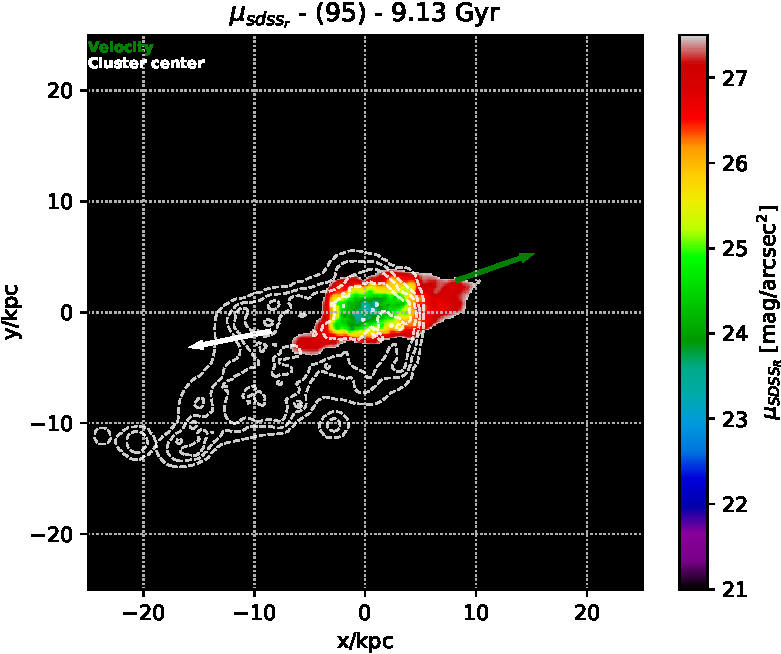
\includegraphics[width=\columnwidth]{69p100_0095_sb-crop.pdf}
% \caption{Surface brightness map with superimposed \Hi{} density contours with 5 equidistant in log-scale levels from $10^{17}$ to $10^{22}$ atoms/cm$^2$.}
% \label{fig:sb}
% \end{figure}

\section{Simulations} \label{sec:simulations}
\begin{figure}
\centering
\begin{subfigure}[b]{0.49\textwidth}
 \centering
 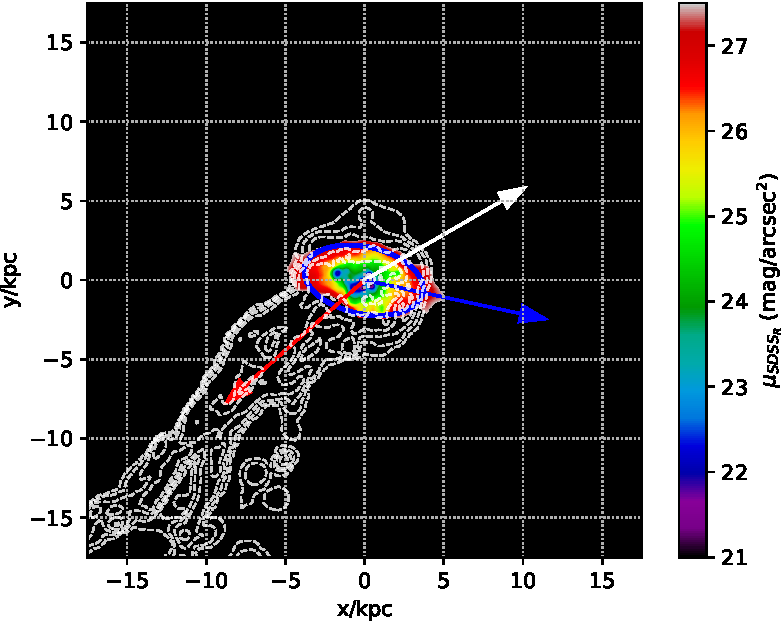
\includegraphics[width=\textwidth]{NGC_LIKE/SB.pdf}
 \caption{}
 \label{fig:sb_arrows}
\end{subfigure}
 \hfill
  \begin{subfigure}[b]{0.5\textwidth}
  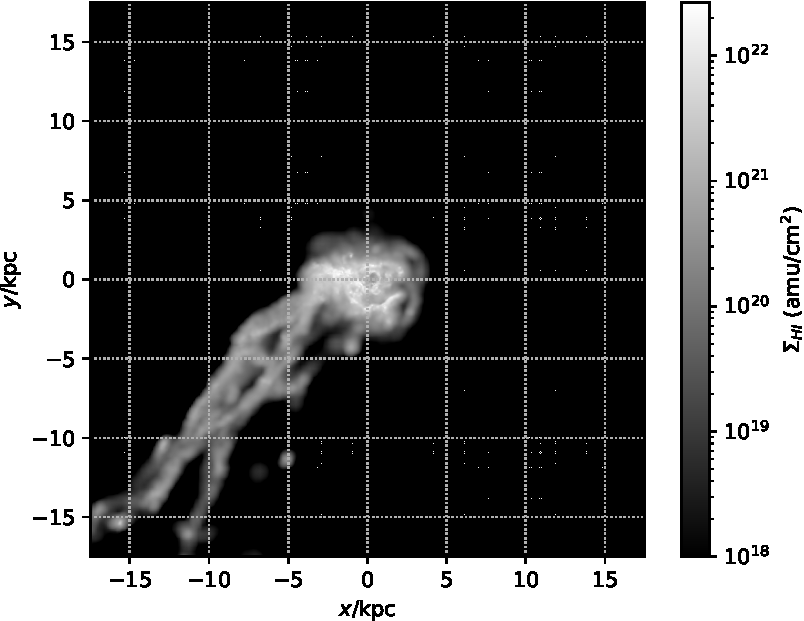
\includegraphics[width=\textwidth]{NGC_LIKE/HI.pdf}
  \caption{}
  \label{fig:sim_hi_density}
\end{subfigure}
\hfill
\begin{subfigure}[b]{0.5\textwidth}
  \centering
  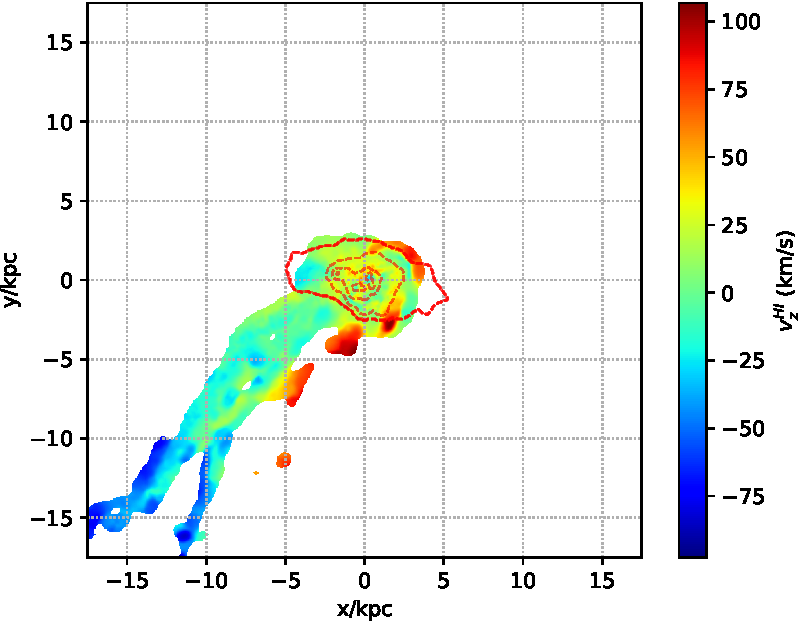
\includegraphics[width=\textwidth]{NGC_LIKE/HI_VEL.pdf}
  \caption{}
  \label{fig:sim_hi_kin}
\end{subfigure}
 \vfill
\caption{A simulation snapshot (ID 68, see Table \ref{tbl:sim}) on an orbit with 100 kpc pericenter distance, showing stellar tidal and gaseous stripped tails.
(a) $r'$-band surface brightness with \Hi{} column density contours as seen from a point of view for which the projected cluster-centric distance $r_p = 77$ kpc and the recessional velocity $-793$ km/s. 
\Hi{} contours are drawn at column density levels [$10^{17}, 10^{18}, 10^{19}, 10^{20}, 10^{21}$]~amu~cm$^{-2}$. The white arrow points towards the cluster center, whereas the blue and the red arrows are the computed orientation of the stellar tail and the gaseous tail respectively, see Section \ref{sec:morphological_quest}.
%(same as \citet{Lee-Waddell2018})
(b) The column density of the neutral hydrogen, highlighting clumpy blobs of stripped \Hi{}.
(c) SPH map of the \Hi{} velocity field where the \Hi{} tail in its rightmost part is receding more than the more detached part.
For reference, the [22, 24, 26, 28]~mag/arcsec$^2$ isophotes are shown as dashed red contours.
We stress that our Fornax cluster dwarf galaxy simulations were not designed to reproduce all the details of this particular galaxy. Nonetheless, remarkable similarities can be found.} 

\label{fig:selected_snapshot}
\end{figure}

The simulations used in this chapter are described in full details in \refsec{sec:fornax_sim}. We stress that they have not been set up to mimic NGC~1427A in any particular way. Therefore, not all details can be expected to exactly match with observations.
Nonetheless, these simulations provide valuable insights not only into the phenomena at play but, more importantly, they can be used to infer the most likely current orbital phase of the galaxy. 


\section{Constraining the orbital phase of NGC~1427A} \label{sec:results}

\subsection{Quantitative morphological search}
\label{sec:morphological_quest}

We carried out a systematic search among all the simulation snapshots, portraying different dwarfs at different times on different orbits.
We observed each snapshot from different points of view in order to select the snapshots and their orientation most resembling the observed galaxy using four measurable quantities:
\begin{enumerate}
    \item[(i)] the projected cluster-centric distance, $r_p$;
    \item[(ii)] the line-of-sight velocity with respect to the cluster center,~$v_p$;
    \item[(iii)] the position angle of the outer isophotes, quantified as the angle $\alpha$ between the projected cluster center direction and the direction of the $26.5$~mag/arcsec$^2$ isophote in $r'$ band, see Figure~\ref{fig:angles_scheme};
    \item[(iv)] the orientation of the \Hi{} tail as measured with the angle $\beta$ between the isophote orientation and the direction of the highest variance of the image obtained by computing the second order moments of the \Hi{} SPH map \citep{Stobie1980}.
\end{enumerate}
\begin{figure}
\centering
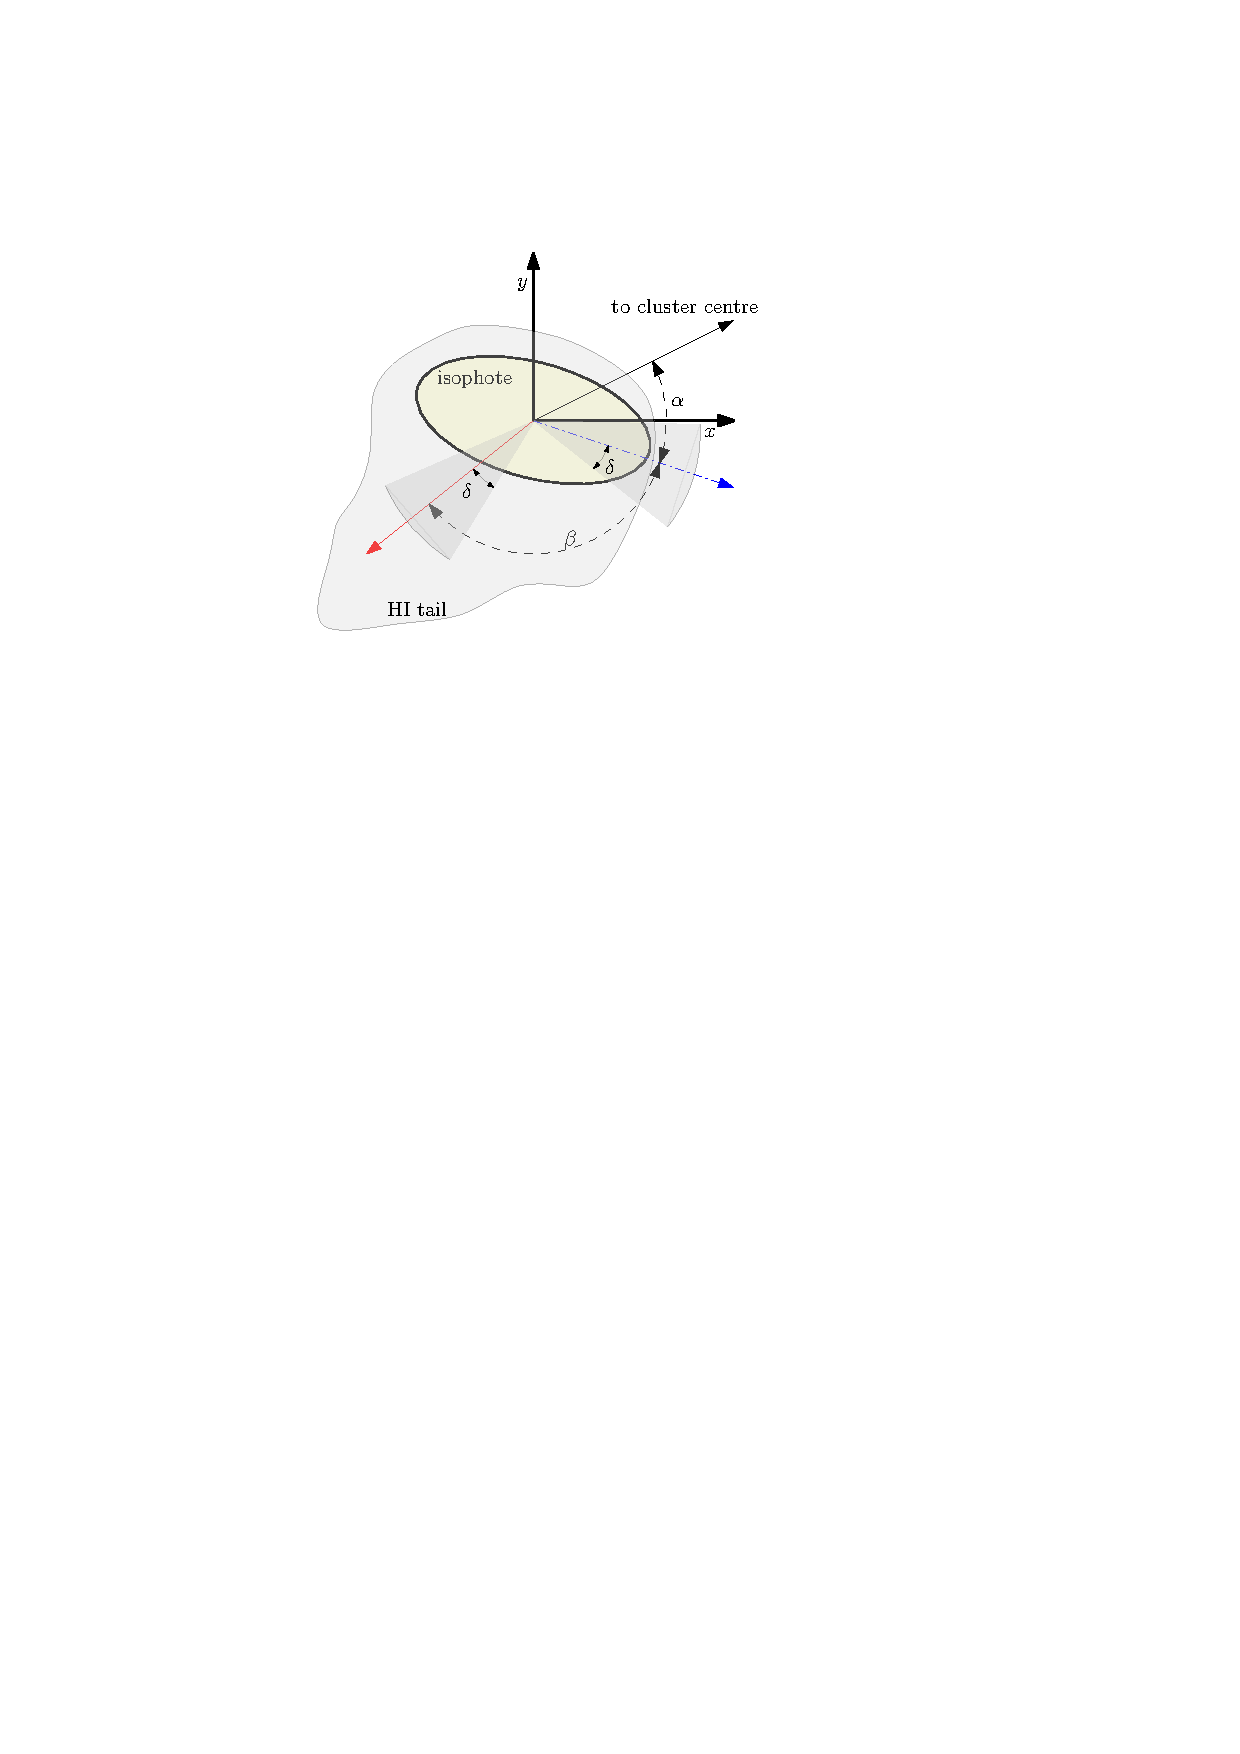
\includegraphics[width=0.65\columnwidth]{alpha_beta_coloured_for_fig.pdf}
\caption{Angles $\alpha, \beta$ definitions used to set up the  requirements for the morphological search. $\delta$ is the angle tolerance used for the selection. Blue and red arrows are defined as in Figure \ref{fig:sb_arrows}. Darker grey shaded regions are the allowed directions of the oriented snapshots tidal stellar tail and \Hi{} tail.}
\label{fig:angles_scheme}
\end{figure}
\begin{figure}
\centering
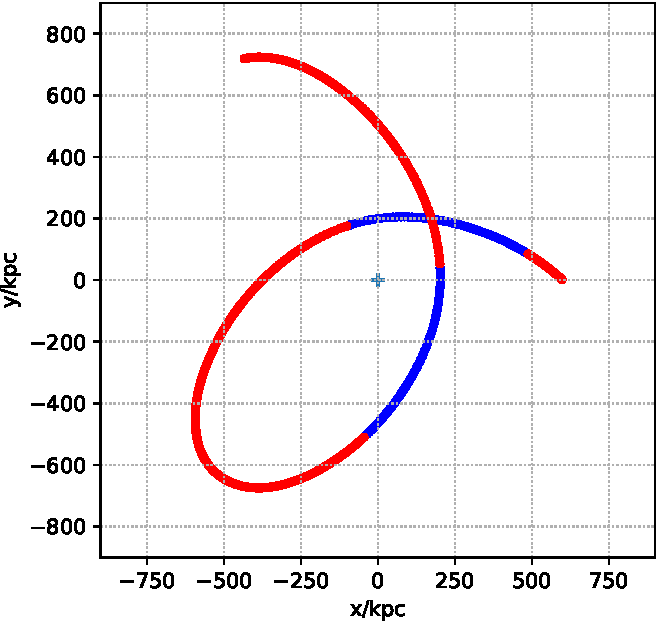
\includegraphics[width=0.55\columnwidth]{good_traj.pdf}
\caption{A trajectory with pericenter of 200~kpc. In blue the orbital phases for which there are snapshots with projected distance and recessional velocity compatible with the ones of NGC~1427A (i.e. snapshots fulfilling requirements (i)-(ii)) for some points of view.
In this case $r_p = 137$~kpc, $v_p = -693$~km/s.}
\label{fig:good_traj}
\end{figure}
We highlight that the search has been carried out using only morphological and orbital parameters, given our focus on the peculiar morphology of NGC~1427A.
Moreover, the criteria used to compare simulations to observations are the ones that best represent the effects of the cluster environment: the relative directions of the tidal pull and the ram pressure stripping. Indeed, the first two requirements put constraints on the orbital position and hence on the orbital phase of the simulated dwarf. The latter two require that the isophotal tail and the neutral gas tail are oriented as in NGC~1427A.
By selecting a faint isophote for criterion (iii) we are tracing the outer tidal extensions of the stellar body.
Inspection of the evolution of the direction of the principal axes of the stellar density distribution along a simulated dwarf galaxy's orbit shows that the galaxy outskirts rapidly forget their initial spatial orientation and become strongly aligned with the cluster center around pericenter and apocenter. On the inward or outbound legs of a galaxy's orbit, this elongation occurs parallel with its orbital velocity. This evidence for a tight correlation between a dwarf galaxy's elongation and its orbital phase, led us to include criterion (iii).

From VST images of \citet[][]{Lee-Waddell2018} \citep[originally from the deep survey presented in][]{Iodice2016} we used the position angle of 15~deg of the fitted ellipse in its Figure 2.
From the \Hi{} maps of Figures 1 and 3 of the same paper (see Figures \ref{fig:hi_contours} and \ref{fig:hi_kin} above) we assumed an inclination of the \Hi{} tail of -135~deg (pointing south-east).
%, see Figure \ref{fig:arrows}.
Given that the direction of the cluster center is around 30~deg north-west, the resulting target angles are $\bar \alpha = 45$~deg, $\bar \beta = 120$ deg, as in Figure~\ref{fig:angles_scheme}.

For each snapshot, we started by finding the orbital phase which fulfils the first two requirements.
Each requirement is satisfied by the set of points of view constituting the generatrices of a cone centered on the galaxy position.
By intersecting two cones it is possible to find the points of view satisfying the requirements.
This is equivalent to solving a quadratic equation (see section \ref{sec:cone_intersection}) whose two solutions are two points of view satisfying the requirements (i) and (ii).
Each snapshot is then rotated as if it was observed from the peculiar point of view yielding the imposed clustercentric distance and the recessional velocity.
The more radial the orbit is, the higher the number of suitable snapshots which will be further selected using requirements (iii) and (iv), see Figure \ref{fig:good_traj}.

With the assumed cluster center at a distance of 20~Mpc from us (see Section \ref{sec:intro}), we imposed as targets the two quantities $\bar r_p=137$~kpc and $\bar v_p=-693$~km/s with measures for NGC 1427A (the projected distance on the sky and recessional velocity of NGC~1427A w.r.t. NGC~1399).
In order to take into account uncertainties in the measured $\bar r_p$ and $\bar v_p$ and to capture the sensitivity of the procedure to the selected projected distance and recessional velocity, we repeated the same procedure for each simulated snapshot but allowing for other slightly offset targets $r_p$ an $v_p$.
Practically, we fixed an offset in both quantities $r_p = \bar r_p \pm \Delta r$, $v_p = \bar v_p \pm \Delta v$ with $\Delta r = 100$ kpc, $\Delta v = 60$ km/s.
Also we added four other targets: $(\bar r_p \pm \Delta r, \bar v_p)$ and $(\bar r_p, \bar v_p \pm \Delta v)$ with same ($\Delta r, \Delta v$) as before.
Including the exact target $\bar r_p, \bar v_p$, at the end, we had nine targets to check for each snapshot.
In total, we obtained a dataset of 424,656 oriented snapshots.

For each snapshot surviving the selection of requirements (i) and (ii) and oriented so that $r_p$ and $v_p$ are the ones imposed, we created the surface brightness map and \Hi{} map.
We first fitted an ellipse to the contour corresponding to the $26.5$~mag/arcsec$^2$ isophote in $r'$ band.
We computed the second order moments of the \Hi{} map to obtain the direction of the neutral hydrogen tail.
Since we are interested in snapshots with an elongated \Hi{} tail in the South-East direction, we further selected only oriented snapshots with galactic projected velocity on the plane of the sky having a positive projection on the cluster center direction. This removes false positives with a \Hi{} tail inclined with the proper angle but extending towards the cluster center (from the image moments only the direction is returned, not the sense of elongation of the tail).
At the end of this pre-selection, we ended up with 59,896 oriented snapshots.

We then used requirements (iii) and (iv) to further refine the search.
In the following section we shall determine the distribution of the snapshots with tails similar to the observed galaxy using angles $\alpha$ and $\beta$, described above, and a tolerance $\delta$:
\begin{equation*}
\bar \alpha - \delta < \alpha < \bar \alpha + \delta, \qquad
\bar \beta - \delta < \beta < \bar \beta + \delta
\end{equation*}
The selection tolerance $\delta$ is then our main knob to filter-out snapshots oriented as NGC~1427A with angles $\bar \alpha$ and $\bar \beta$. The dependence of the results (and the number of oriented snapshots surviving the selection criteria (i-iv)) on its choice is quite strong, so in all the following histograms we highlight the $\delta$ chosen.


\subsection{Finding points of view - cones intersection}
\label{sec:cone_intersection}
Finding the point of views from which the galaxy appears as having the target projected clustercentric distance ($r_p$) and the proper line-of-sight velocity ($v_p$) is equivalent to solving the problem of intersecting two cones.

Given $\vec x$ the unit vector representing the direction of the point of view, and $\vec r$ and $\vec v$ the clustercentric position and velocity of the galaxy respectively, we can write the following conditions:

\begin{equation}
\label{eq:system}
\begin{cases}
\vec x \cdot \vec v = v_p\\
\vec x \cdot \vec r = \pm R\\
|\vec x|^2 = 1
\end{cases}
\end{equation}
where $R = \sqrt{r^2 -r_p^2}$. By using [$\vec r, \vec v, \vec r \times \vec v$] as basis (right-handed but not orthogonal), it is possible to express $\vec x$ as:
\begin{equation}
    \vec x = a \vec v + b \vec r + c ( \vec r \times \vec v).
\end{equation}
Substituting into \eqref{eq:system}:
\begin{equation}
\begin{cases}
a v^2 + b (\vec r \cdot \vec v) = v_p\\
a(\vec r \cdot \vec v) + b r^2 = \pm R\\
|\vec x|^2 = 1 = a v^2 + b r^2 + c^2 | \vec r \times \vec v|^2 + 2 ab(\vec r \cdot \vec v)
\end{cases}
\end{equation}
The last quadratic equation yields immediately two values of $c$ ($c_1$, $c_2$).

For each chosen sign of $R$, the system yields two solutions: ($\vec x_1$, $\vec x_2$) which can be used to rotate the galaxy snapshot as if it was seen from the directions $\vec x_1$ and  $\vec x_2$.

Each direction can be defined using two angles ($\varphi$ and $\theta$) representing the spherical coordinates of the unit vectors $\vec x_1$ and $\vec x_2$.

\begin{figure}
  \centering
  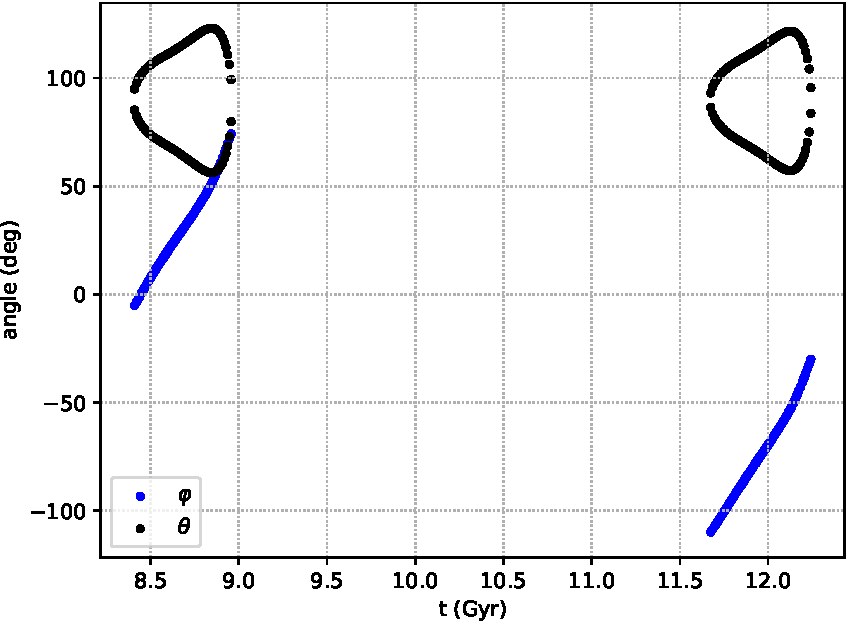
\includegraphics[width=0.8\columnwidth]{angles.pdf}
  \caption{Angles $\varphi, \theta$ defining the points of view of each snapshot of the trajectory of Figure \ref{fig:good_traj}. The angles are used to rotate the selected snapshots in order to obtain the target $r_p, v_p$. Only a subset of snapshots can be oriented to fulfil the requirements.}
  \label{fig:phitheta}
\end{figure}
In Figure \ref{fig:phitheta} an example of rotation angles for a particular simulated orbit is shown.
The angles $\varphi$ and $\theta$ are used to rotate the simulated galaxy as if it was observed from the peculiar point of view yielding the imposed clustercentric distance $r_p$ and the recessional velocity $v_p$.


\subsection{Distribution along the orbit of points of view satisfying the requirements}
\begin{figure}
\centering
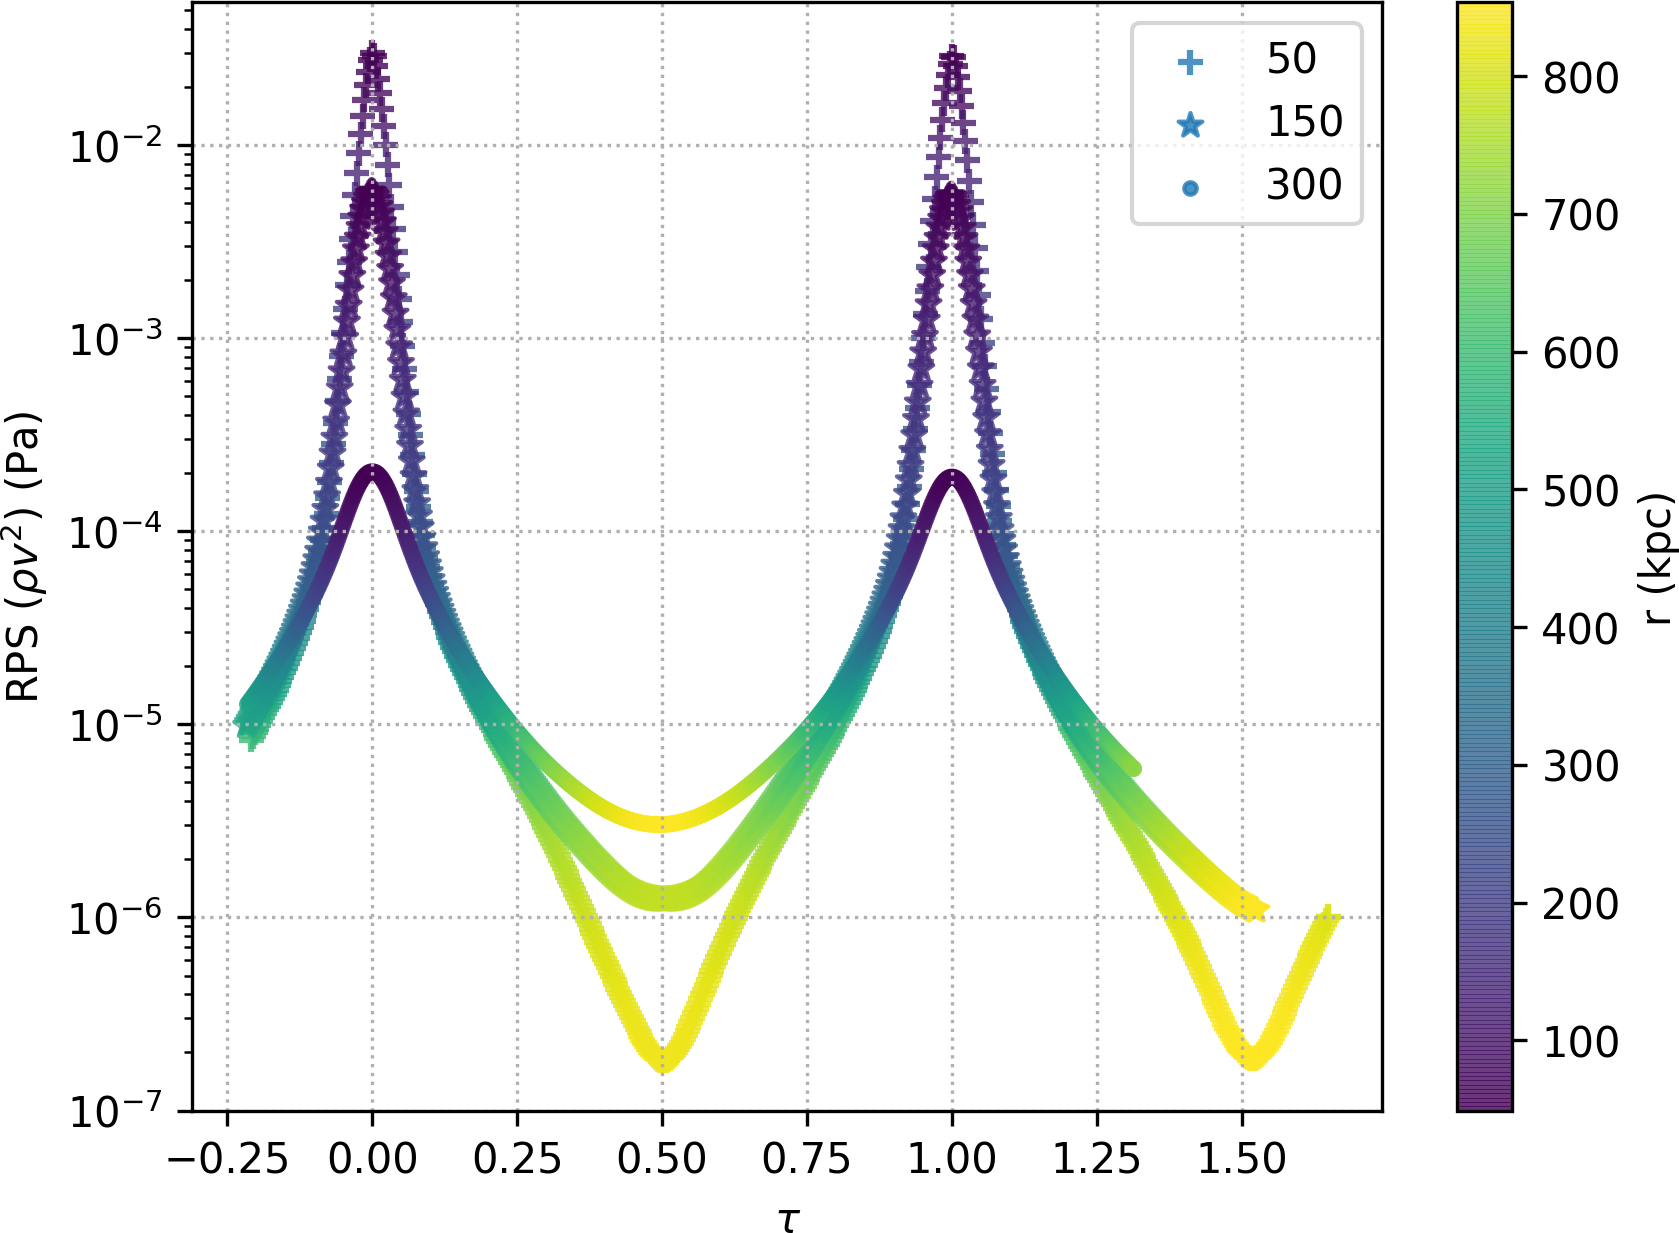
\includegraphics[width=0.8\columnwidth]{rps-crop.png}
\caption{The strength of the ram pressure ($\rho v^2$) as a function of normalised time $\tau = (t-t_p)/T_r$, where $t_p$ is the time of first pericenter passage and $T_r$ is the orbit's radial period, for the ID 69 simulations on multiple orbits (orbit pericenter in kpc is indicated in the legend). The colour scales traces orbital distance with respect to the cluster center.}
\label{fig:r_rps}
\end{figure}
We computed the distribution of selected oriented snapshots with respect to the time from the pericenter passage.
We noted that all the snapshots surviving the selection are found within 200 Myr of a pericenter passage.

We ascertain the robustness of this result by varying the tolerance~$\delta$ of the comparison of the angles $\alpha, \beta$ with the observed ones.
Our orbital and morphological criteria are preferentially met by simulations with a stellar mass above $ \approx10^8 $ \Msun{}.
Less massive galaxies and galaxies on radial orbits are completely stripped from their HI gas, see Figure \ref{fig:m_hi}, because of the steep increase of ram pressure around pericenter as shown in Figure \ref{fig:r_rps}.
\begin{figure}
\centering
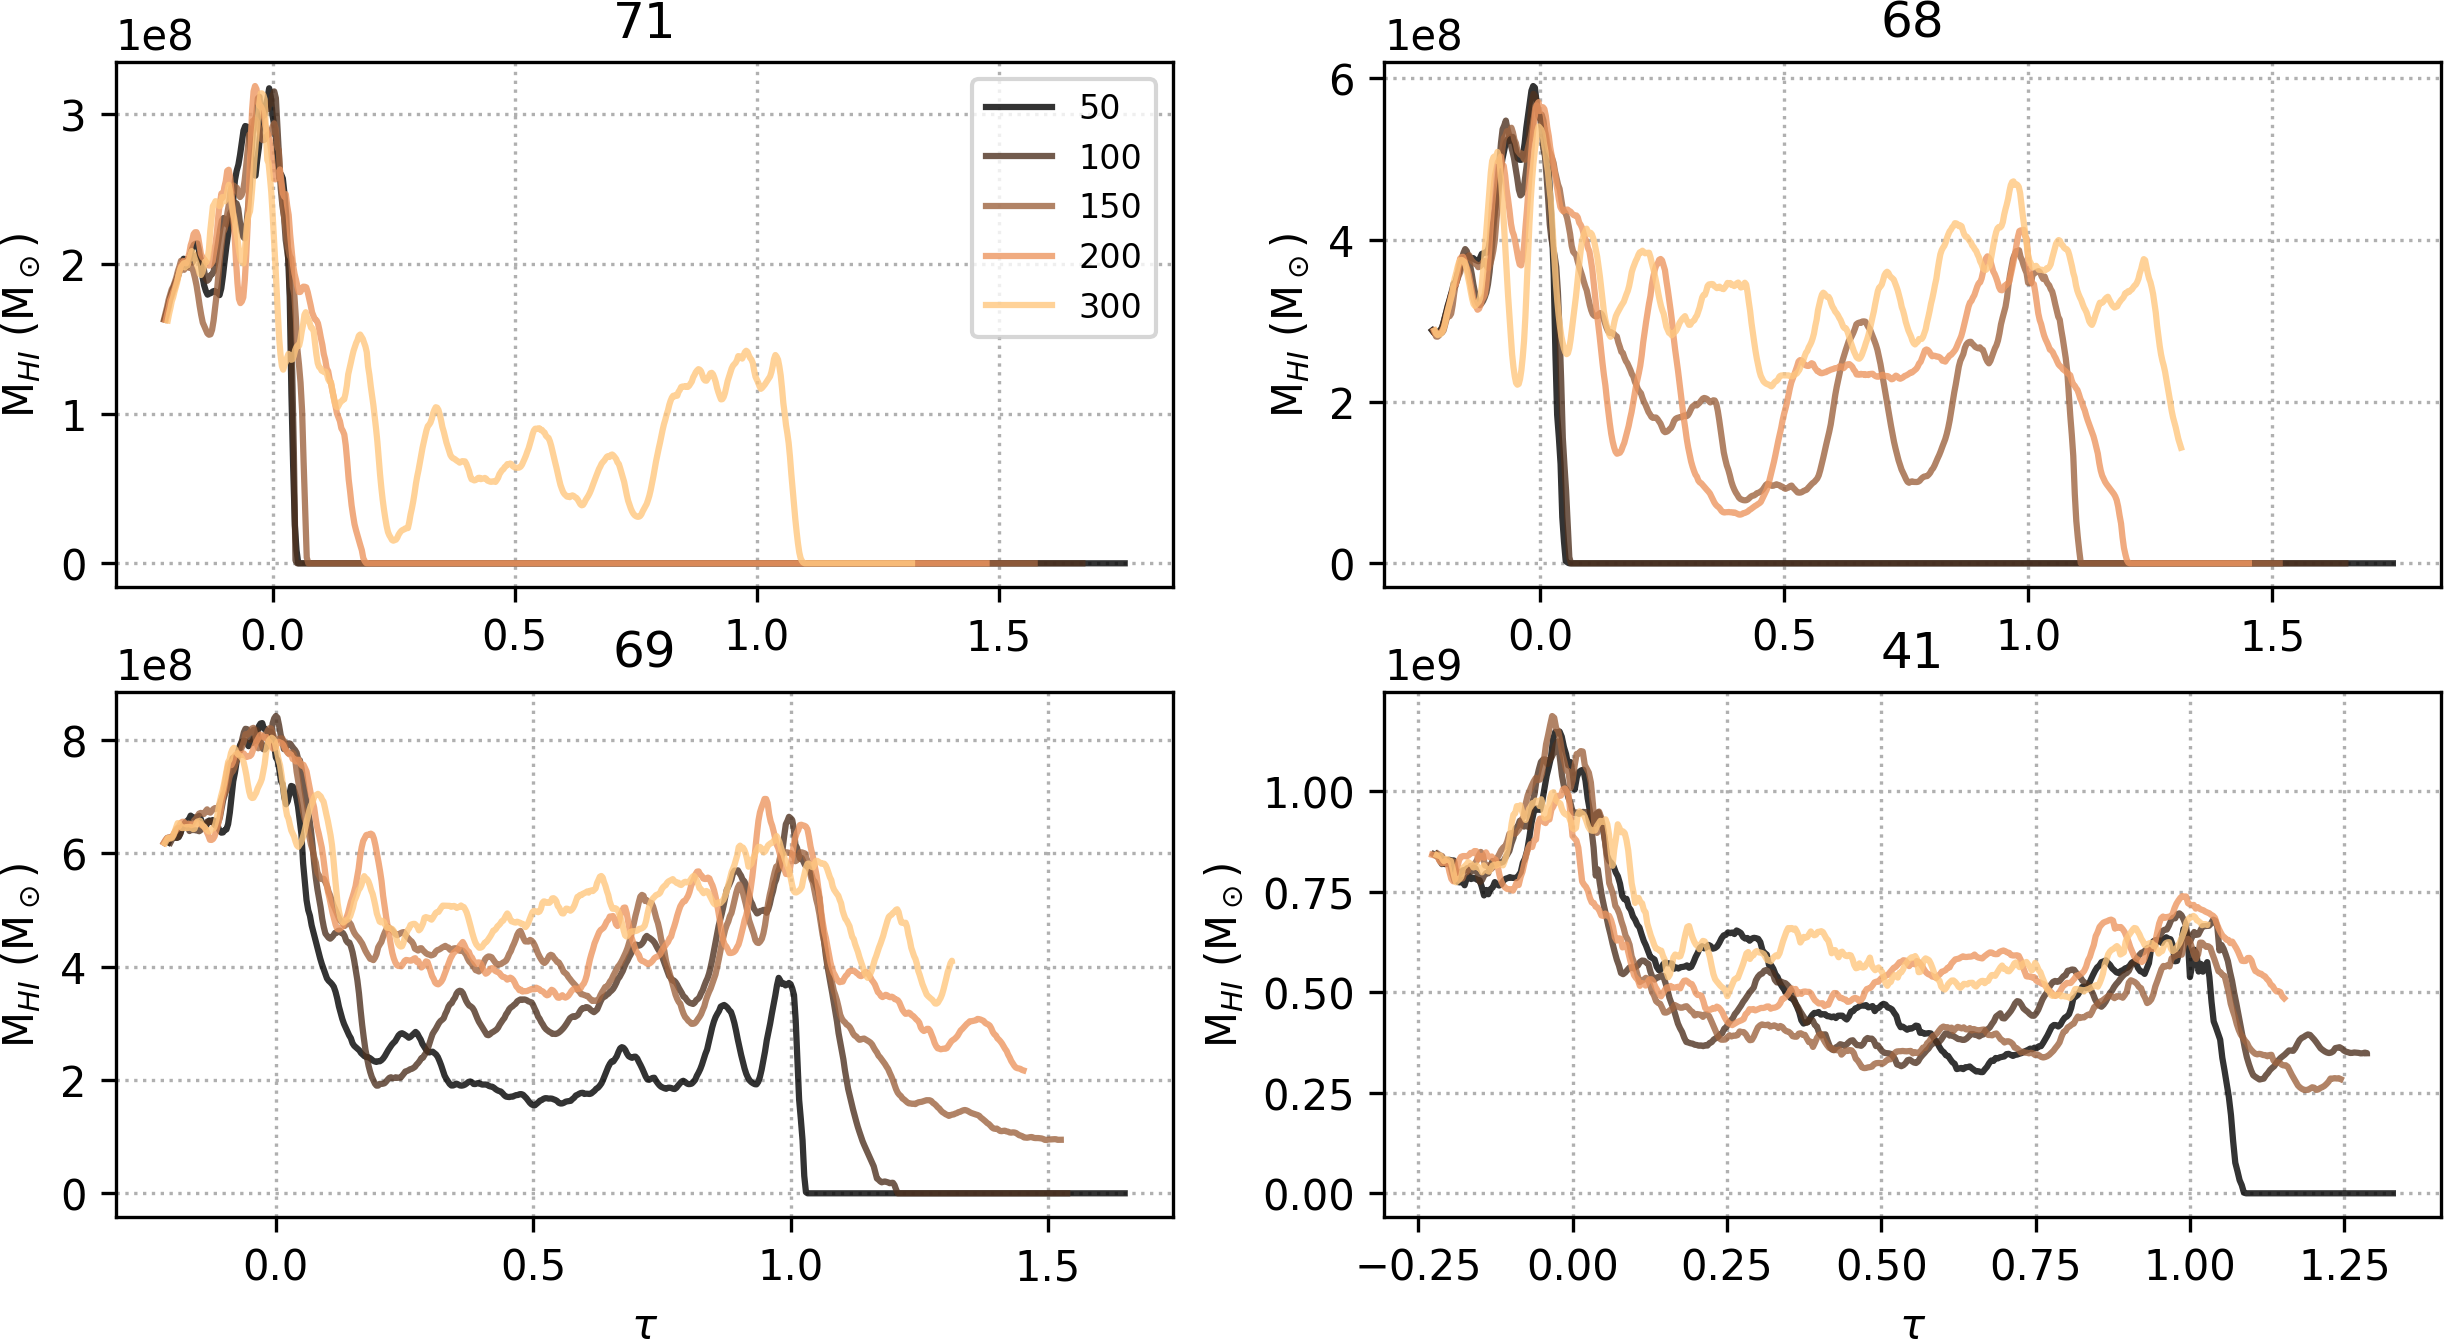
\includegraphics[width=\textwidth]{m_hi-crop.png}
\caption{Neutral gas mass as a function of normalised time $\tau$ as defined in Figure \ref{fig:r_rps}.
Each panel is labelled with the simulation ID (cf. Table~\ref{tbl:sim}) and contains information for the simulated dwarf launched on orbits with different pericenter distances (50, 100, 150, 200, 300 kpc identified by the colour legend in the top-left panel). Gas is compressed when the isolated galaxy enters the cluster and as a consequence it cools down, thus increasing the neutral hydrogen mass. Obviously, around pericenter, ram pressure stripping is effective at driving down the gas mass (as shown also in Figure~\ref{fig:r_rps}).
}
\label{fig:m_hi}
\end{figure}
Especially for radial orbits, no oriented snapshot is found on orbits of 50 and 100 kpc after first pericenter passage, regardless of the tolerance~$\delta$ considered, as shown in Figure~\ref{fig:histo_peri}.
For the most circular orbits, only snapshots undergoing second pericenter passage survive the selection. This is likely due to the first passage acting as `preprocessing' and making the galaxy potential shallow with higher chances to create tidal tails.
% \todo{I'm currently having a look at the distribution of ellipticity of the fitted isophotes to see how circular, and hence not so tidal, they are. Update: See figure noperi_all_stacked-crop.png }
In Figure~\ref{fig:histo_noperi} we performed the same analysis cumulatively counting all the oriented snapshots (without pericenter distance distinction) but using different isophotes.
The diagrams, even if noisier when using fainter isophotes, convey the same message: there is an abundance of correctly oriented snapshots (with tails as NGC~1427A) around first pericenter passage.
Indeed, tidal tails as those shown in Figure~\ref{fig:panel}, are present in low surface brightness regions of the dwarf, even if they are more difficult to measure.
The counterpart in NGC~1427A would be the faint stellar South-West elongation visible especially in $r'$-band, see Figure~\ref{fig:r_band}.

\begin{figure}
\centering
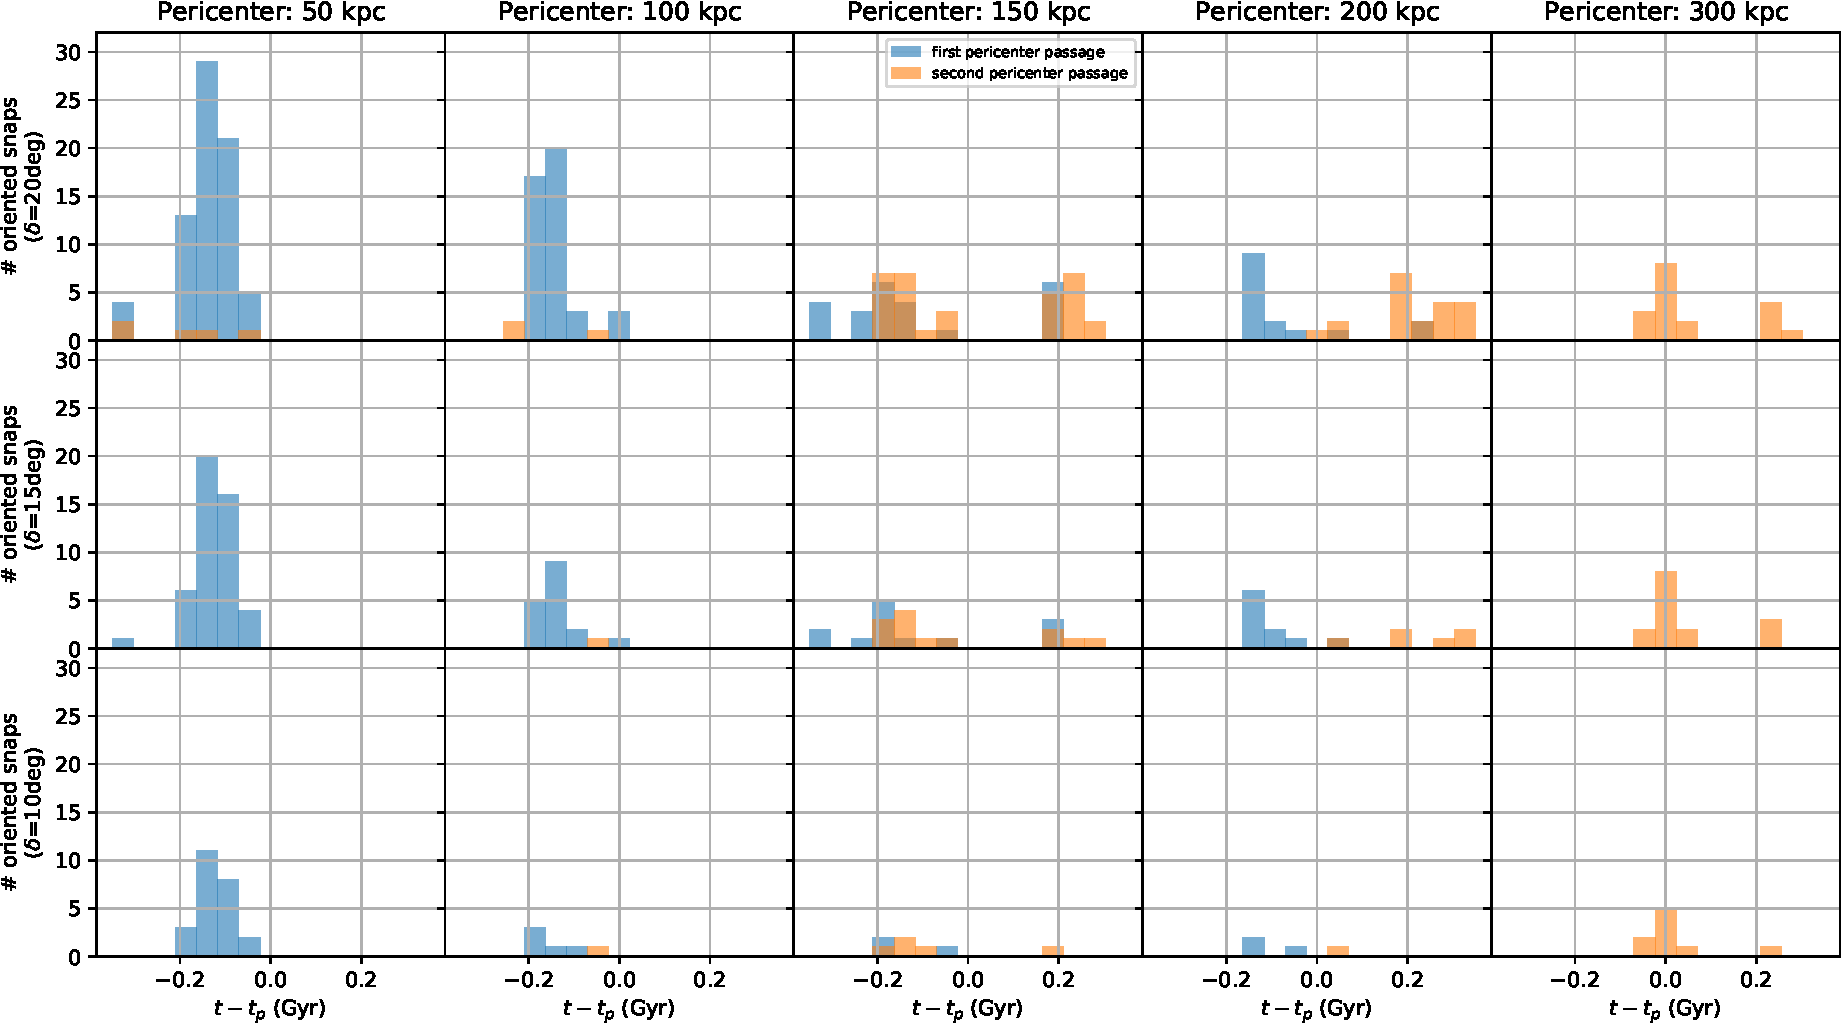
\includegraphics[width=\textwidth]{histo/histo_iso26.5_bins0.35-16.pdf}
\caption{Histograms of oriented snapshots fulfilling the requirements (i)-(iv), selected to be around first (blue) or second (orange) pericenter and grouped by orbital pericenter distances (50, 100, 150, 200, 300 kpc).
The isophote used to compute the stellar tail inclination is $26.5$~mag/arcsec$^2$ in $r'$ band.
The distribution is peaked at around 150 Myr before pericenter passage, especially in more radial orbits. The result is robust enough to be visible on stricter angle tolerances $\delta = [20, 15, 10]$~deg.
}
\label{fig:histo_peri}
\end{figure}

\begin{figure}
\centering
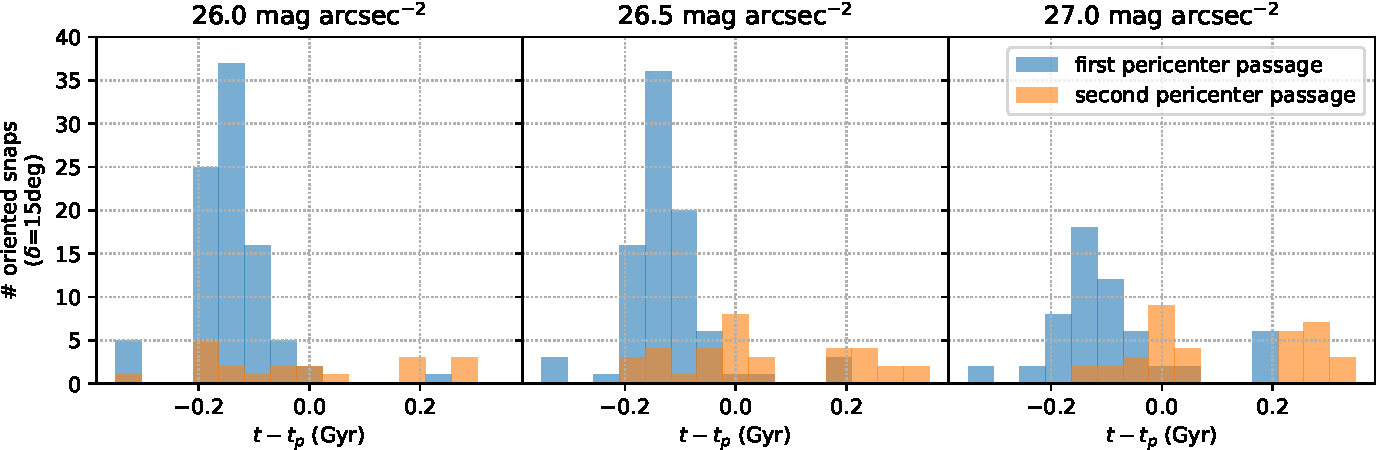
\includegraphics[width=\textwidth]{histo/iso_comparison_tol15_asym0.0_bins0.35-16.pdf}
\caption{Distribution in time relative to pericenter passage of oriented snapshots fulfilling the requirements (i)-(iv) with tolerance $\delta=15$ deg.
Histograms of selected snapshots are coloured relative to their orbital phase: around first (blue) or second (orange) pericenter.
Each column corresponds to a different isophote used to compute the stellar tidal orientation.
Irrespective of the isophote, the distribution remains peaked  around 150 Myr before pericenter passage.}
\label{fig:histo_noperi}
\end{figure}

\subsection{3D position of the galaxy in the Fornax context}

Based on the above described model, we can produce a quantitative estimation of the galaxy projected radial distance. This measure is actually a testable prediction with distance observations.
Unfortunately, current uncertainties on the distance measurements do not allow to unequivocally assess the position of the galaxy to be in front or behind the cluster center \citep{Georgiev2006}.

Using our models we can see which is the most likely radial distance relative to the cluster center of a galaxy with morphological features like NGC~1427A.
As shown in Figure \ref{fig:distance_prediction}, the preferred line of sight distance is around 200~kpc in front of the cluster center.

It is also possible to compute the flight angle $\gamma$ of the galaxy with respect to the line of sight direction (see Figure \ref{fig:gamma}).
As shown in Figure \ref{fig:velocity_prediction}, from the above models, the most frequent is $\gamma\approx 50$~deg.
Given that the stripped gaseous tail approximately follows the opposite direction of flight, measuring the flight angle in simulations can be useful to assess the real length of the gaseous tail in observations.
Our result would indicate the real tail to be roughly a factor 1.3 longer than the projected one.

\begin{figure}
\centering
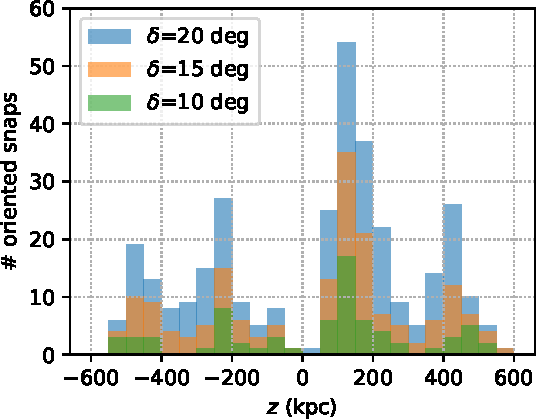
\includegraphics[width=0.8\columnwidth]{histo/multi_tol_dist_gauss_bins600_25.pdf}
\caption{Distribution of selected oriented snapshots with multiple tolerance $\delta$ along the projected line of sight. The zero point is 20~Mpc, assumed distance of NGC~1399. Positive values mean the galaxy being \emph{in front of} the cluster center. 
%Overplotted a Kernel Desity Estimation for the distribution.
}
\label{fig:distance_prediction}
\end{figure}

\begin{figure}
\centering
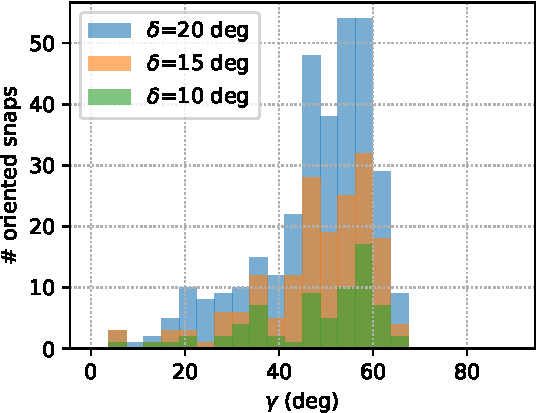
\includegraphics[width=0.8\columnwidth]{histo/multi_tol_vel_angle_bins_gauss90_25.pdf}
\caption{Distribution of the flight angle $\gamma$ of selected oriented snapshots with multiple tolerances $\delta$. $\gamma$ is defined as the angle between the galactic velocity vector in the the cluster reference frame and the line of sight direction. 
%Overplotted a Kernel Desity Estimation for the distribution.
}
\label{fig:velocity_prediction}
\end{figure}
\begin{figure}
\centering
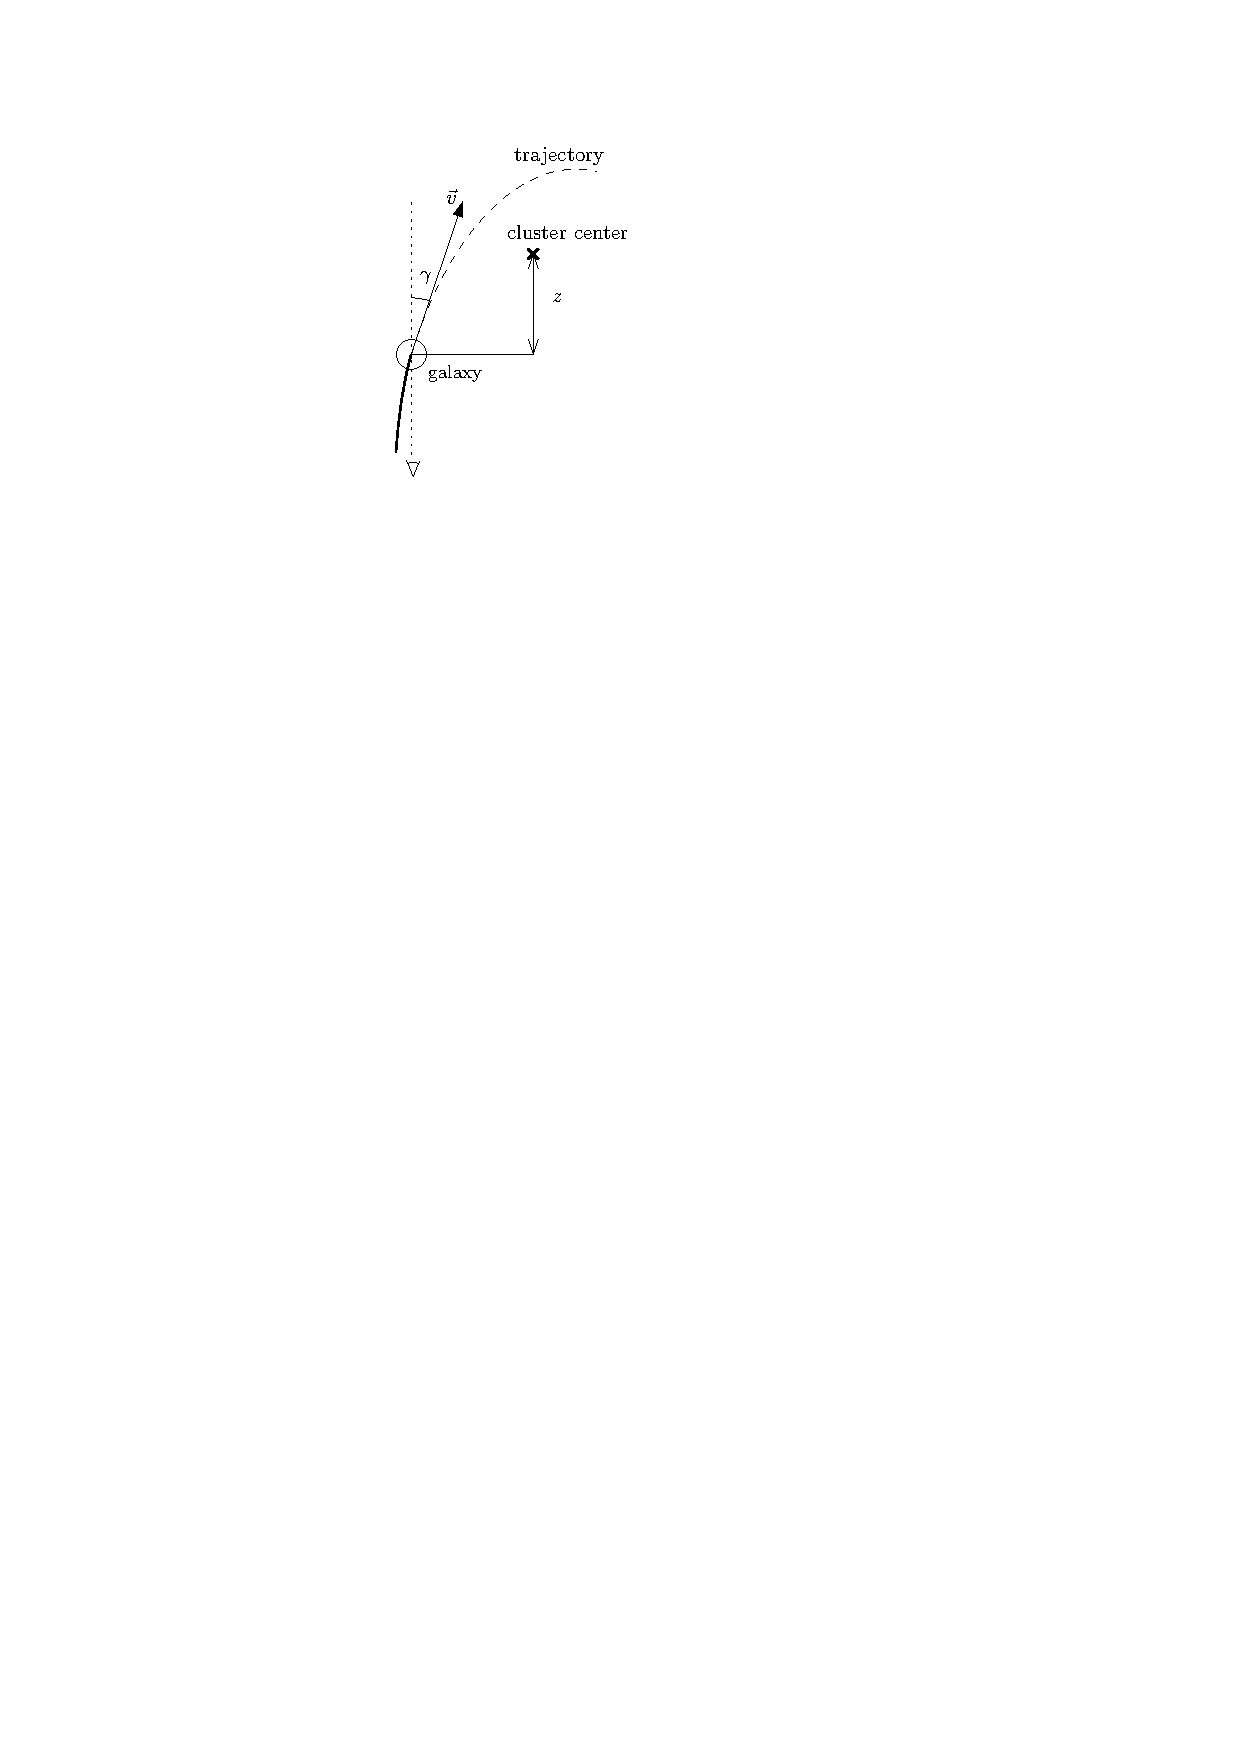
\includegraphics[width=0.5\columnwidth]{gamma.pdf}
\caption{Definitions of angle of flight $\gamma$ and radial distance $z$. $\vec v$ is the orbital velocity of the galaxy.
}
\label{fig:gamma}
\end{figure}

\section{Discussion} \label{sec:discussion}

\subsection{The asymmetric stellar tidal tails}

\subsubsection{Including asymmetry as a constraint}
As a way of quantifying the asymmetric stellar tides, we computed the non-parametric measure Asymmetry \citep[as defined by][]{Lotz2004} of our oriented snapshots. For each oriented snapshot we fed its surface brightness map to \verb|statmorph| \citep{Rodriguez-Gomez2019} isolating the region of the map within $27$~mag/arcsec$^2$.
As a reference, \citet{Su2021} find an Asymmetry of $0.23$ for NGC~1427A.
We tried to add the Asymmetry to the constraints described in Section \ref{sec:morphological_quest}. Given that almost all the oriented snapshots have an Asymmetry higher than $0.2$ \citep[in line with the average of $0.53\pm0.22$ for galaxies with intense star formation as reported by][]{Conselice2003}, we find that isolating snapshots at least as asymmetric as NGC~1427A do not affect the results.

By plotting Asymmetry on selected snapshots as a function of time from pericenter, as shown in Figure \ref{fig:histo2d_asym}, it can be seen that selected snapshots closer to the pericenter become more symmetric.
A possible reason of this can be hypothesised in the tidal pull close to the pericenter which squeezes the galaxy elongating it, hence removing asymmetric regions of the galaxies.
Indeed all simulations show an Asymmetry greater than the one of NGC~1427A. We note that this is in line with \citet{Rodriguez-Gomez2019} who find a systematically higher asymmetry for simulated galaxy of Illustris and Illustris~TNG \citep{Vogelsberger2014, Pillepich2018}, especially in the low mass range.
In fact, in a numerical simulation each star particle created represents stars of $\approx 1000$ \Msun{}: a simulated galaxy is always more "granular" than an observed real galaxy due to the limited resolution.

\begin{figure*}
\centering
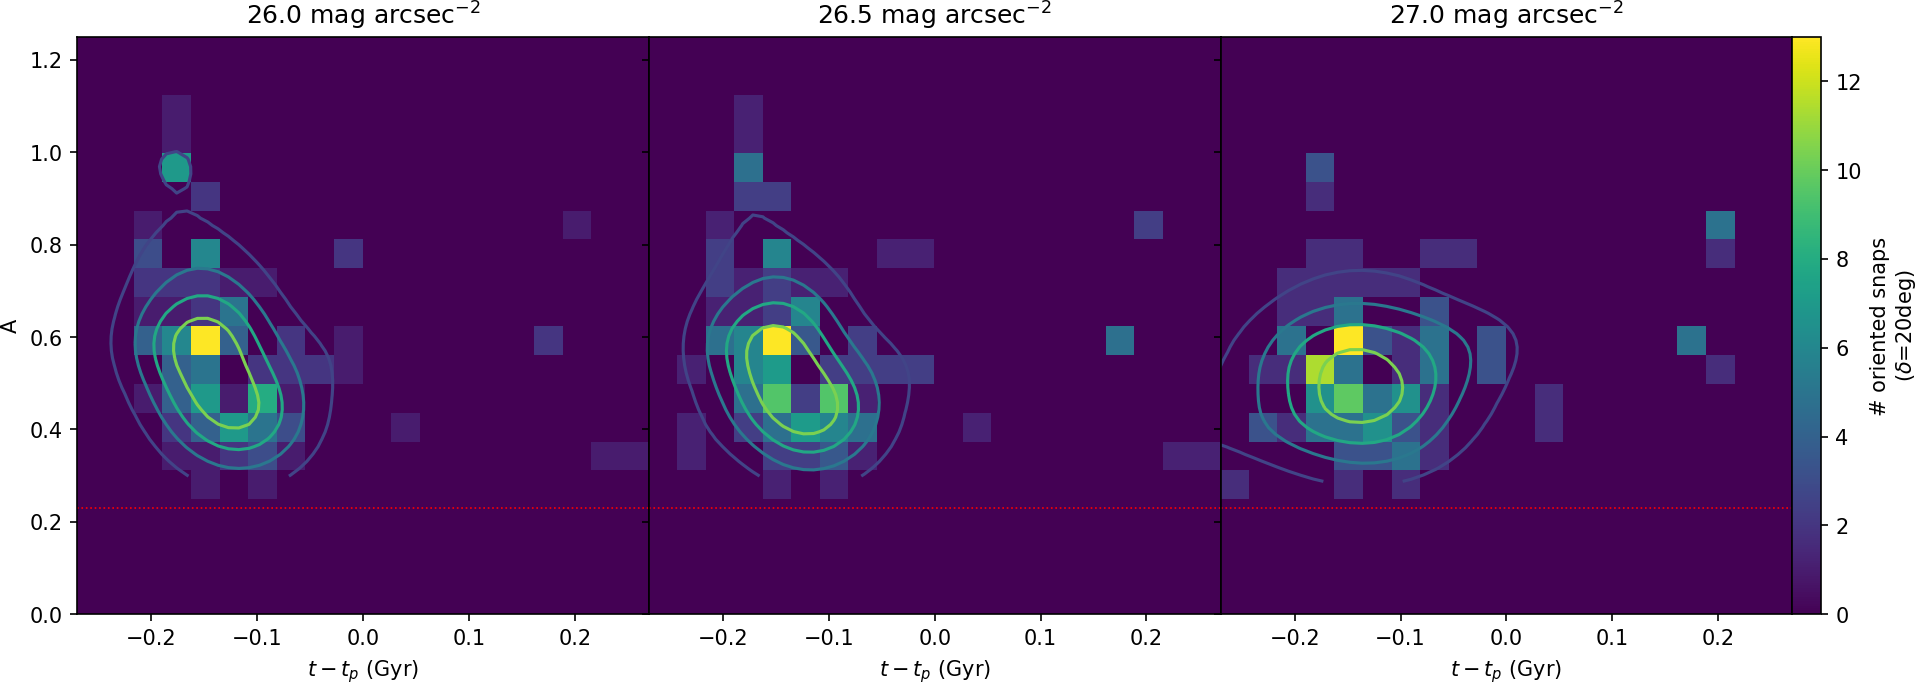
\includegraphics[width=\textwidth]{histo/hist2d_tp_A_bins20_kde-crop.png}
\caption{2D histogram of selected oriented snapshots with tolerance $\delta=20$~deg.
The distribution is plotted with time from first pericenter passage on the $x$ axis, whereas on the $y$ axis the \emph{Asymmetry} non-parametric measure as defined by \citet{Lotz2004}.
Each column corresponds to a different isophote used to compute the stellar tidal orientation.
We overplot a kernel density estimation of the distribution for the snapshots approaching pericenter. The dotted red line corresponds to the measured \emph{Asymmetry} for NGC~1427A.}
\label{fig:histo2d_asym}
\end{figure*}


% \subsubsection{Including isophotal twisting as a constraint}

\subsubsection{The origin of the asymmetric stellar tidal tails}
\begin{sidewaysfigure}
\centering
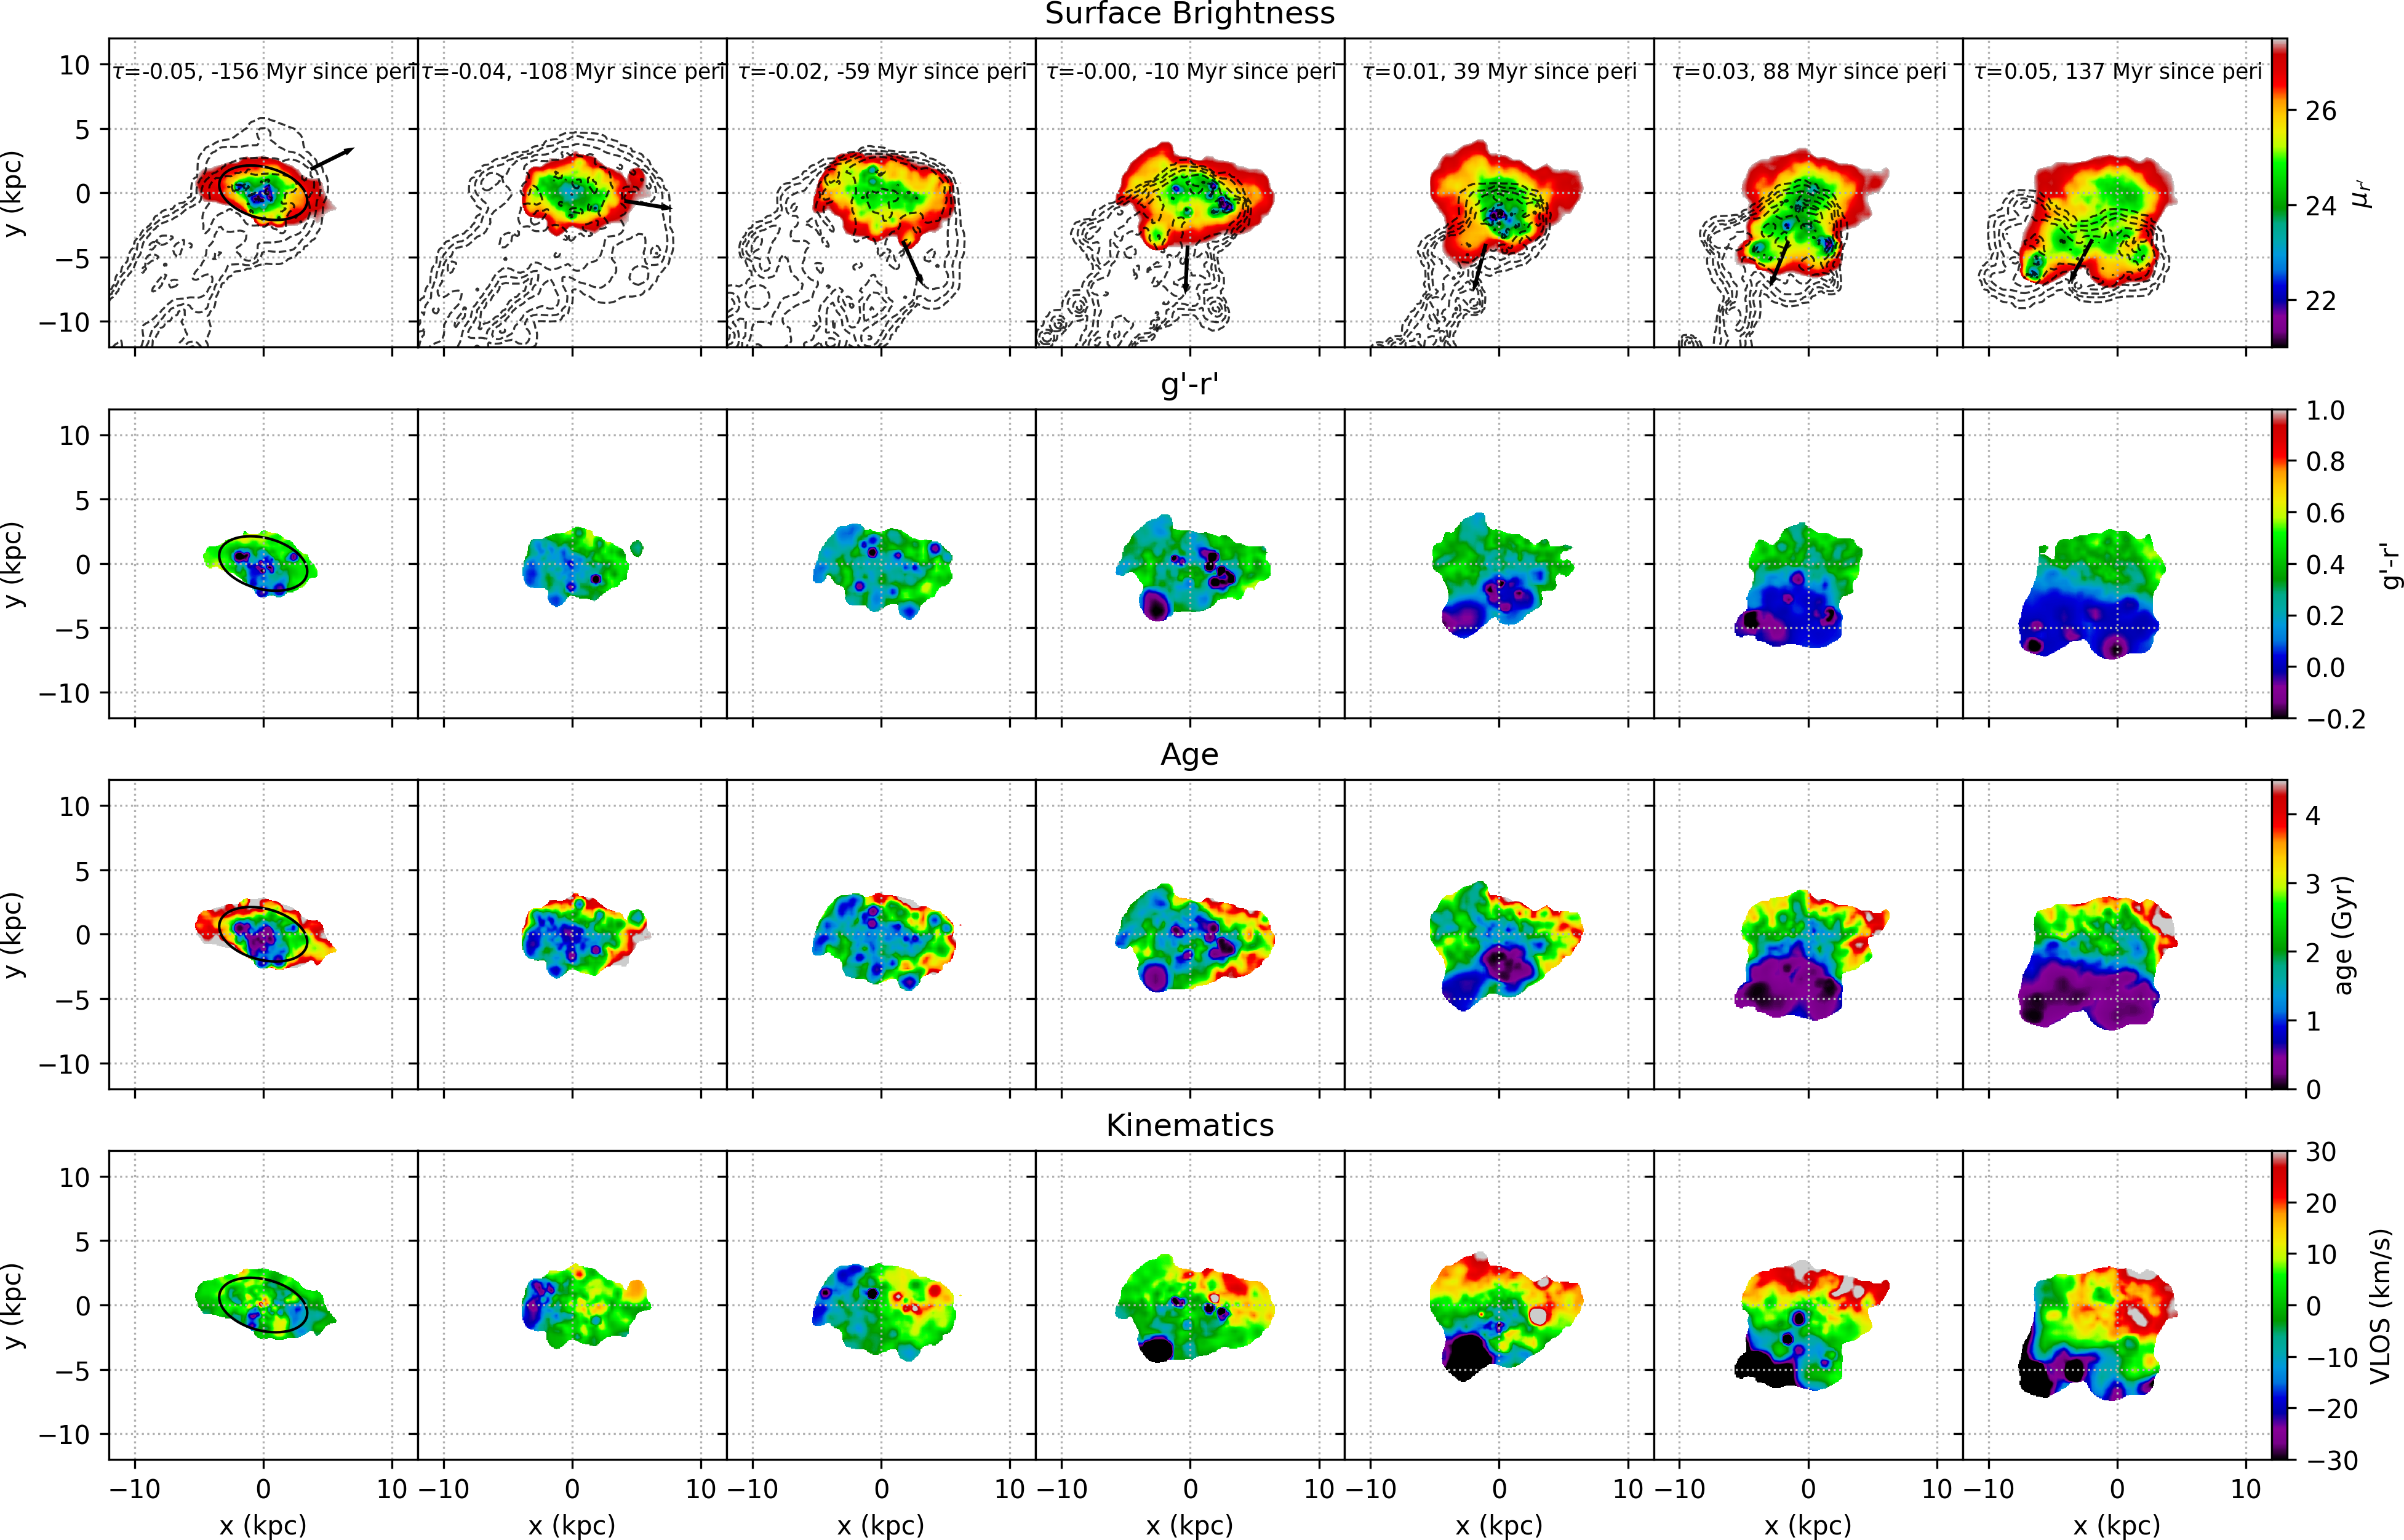
\includegraphics[width=0.95\textwidth]{panel68p100-crop.png}
\caption{Evolution in time of the simulation with ID 68 around first pericenter passage, projected in a way that the first column has $r_p = 137$~kpc, $v_p = 693$~km/s, the target values for NGC~1427A.
All the other snapshots are seen from the same point of view as the first one.
Black arrow indicates the direction to the cluster center whereas the green indicates the instantaneous velocity direction of the galaxy projected on the plane of the sky. In the first column, an ellipse fitted on the $26.5$ mag/arcsec$^2$ is shown to highlight the direction of the tidal elongation.
The first row represents the surface brightness of snapshots around the first pericenter. \Hi{} Contours are [$10^{17}, 10^{18}, 10^{19}, 10^{20}, 10^{21}$]~amu~cm$^{-2}$.
Second row the $g'$-$r'$ colour.
Third and fourth row the v-band SPH-average age and velocity of star particles along the line of sight.}
\label{fig:panel}
\end{sidewaysfigure}

An interesting effect of the pericenter passage is the formation of an asymmetric tidal tail, a stellar elongation more pronounced in just one direction, as that shown in the fourth column of Figure~\ref{fig:panel}.
This effect can be investigated by looking at different simulation snapshots evolving with time around a pericenter passage.
We focus our discussion to the case of the galaxy with ID 68 on an orbit with pericenter $100$~kpc.
In Figure~\ref{fig:panel}, the snapshot in the first column is the one who has passed the filters described in Section~\ref{sec:morphological_quest} and represents a snapshot which is in good agreement to the observation, given its stellar and gaseous tail directions and the projected clustercentric distance and recessional velocity.

We can then reconstruct a series of events leading to the generation of the leading edge stellar tail.
The tidal forces exerted by the Fornax Cluster become markedly asymmetric as a galaxy approaches pericenter on a radial orbit. The steeply deepening gravitational potential well can raise a stronger leading stellar tidal tail while producing a weaker trailing tail during a fast swing-by of a galaxy close to the cluster center. After pericenter, the leading tail twists due to the curvature of the galaxy's orbit, the rapidly changing direction of the gravitational force, and the internal rotation of the galaxy.
Effectively the pericenter passage injects energy into the galaxy resulting in a temporary increase of its angular momentum.

At the same time, the gaseous tail is always directed opposite to the instantaneous velocity.
The result is that the stellar and gaseous tails are very misaligned, almost orthogonal to each other.


\subsection{Possible origin of the Northern Clump in NGC 1427A} \label{NC1427A}
The jellyfish NGC 1427A contains a so called Northern Clump (NC), which has been investigated in detail by some authors \citep{Cellone1997, Hilker1997}.
The NC is a clump of blue and very young stars with associated H$\alpha$ emission \citep{Sivanandam2014}. Even on ground-based images, the NC appears to be composed of two sub-clusters, one to the north of the other. This impression is strengthened by the HST image presented in Figure \ref{fig:NGC1427A}. The centers of the two sub-clusters are separated by 7'', corresponding to just under 700~parsec. The NC lies on NGC~1427A's projected rotation axis and hence its line-of-sight velocity agrees very well with NGC~1427A's mean recession velocity \citep{Bureau1996,Chaname2000}. This does not hint at an external origin for this object. The NC appears to be connected to the north-west rim of the galaxy's main body by a tenuous stream of stars, suggesting it to be displaced along this stream away from the galaxy's main body in a direction that is almost parallel to the major axis of the faint outer isophotes. If, as in our interpretation of the data, these outer isophotes trace the two diametrically opposite stellar tides raised by the Fornax Cluster forces then this would argue for a purely internal origin of the NC. It could be a star-formation region (of which there are many inside NGC~1427A) that is being pulled out by the Fornax Cluster tidal forces, leaving behind a stream of stars.

As shown in Figure \ref{fig:panel}, star formation flares up in our simulated dwarf galaxies around pericenter passage and leads to the appearance of scattered bright, blue clumps of active star formation. These clumps orbit along with the general rotation of their host galaxy. The spatial location and the time of appearance of these clumps are erratic and differ between galaxies and between orbits.
For instance, a star-forming clump is first visible to the top-right of the galaxy in the snapshots 108~Myr before pericenter passage (second column in Figure \ref{fig:panel}; it rotates clockwise, and disappears again after the 137~Myr past pericenter passage snapshot. Likewise, other clumps with similar lifespans pop in and out of existence around pericenter passage. 

Based on these simulations and the available observational data, we suggest that the NC is precisely such a star-forming clump. This interpretation is consistent with its very young age and blue colour, its presence around the time that NGC 1427A is expected to be near pericenter passage (this is required to explain all other characteristics of NGC 1427A), and its kinematics being in line with the galaxy's global velocity field.

%In simulations, as shown in Figure \ref{fig:panel}, around pericenter passage, star formation moves from the galactic center to the gas-rich tail because of ram pressure.
%Many clumps of young stars are therefore formed, suggesting a formation scenario for the Northern Object.
%After pericenter, the galaxy relaxes and stars are being formed again in the galaxy core.

\section{Conclusions}
We carried out a set of simulations of gas-rich late-type dwarf galaxies in a Fornax-like cluster environment.
We isolated snapshots with morphological properties similar to the peculiar galaxy NGC~1427A. The properties have been chosen to be representing the impact of the environment on the dwarf.
We found that the main effects generating peculiar morphology are indeed the combination of ram pressure and tidal interaction close to the cluster center and galaxy rotation.
We saw that the most likely scenario which recreates NGC 1427A tails morphology is assuming the galaxy to be on a very radial orbit with its tail almost aligned with the line of sight, pointing towards the observer.
This naturally leads to a gas kinematic configuration consistent with \Hi{} observations: in the westward part, gas attached to the stellar body of the galaxy is receding whereas the eastward part is stripped and dragged towards the observed by the intra-cluster medium (or ICM), therefore having a smaller recessional velocity, see Figures \ref{fig:sim_hi_kin} and \ref{fig:hi_kin}.

From the analysis of the morphology of the simulated snapshots motivated by environmental effects, we found an excess of snapshots revealing similar NGC~1427A structure around 150 Myr before pericenter passage.
It should be highlighted that this result comes from a suite of simulation which has not been tailored from the beginning to reproduce NGC~1427A.
Nonetheless, interestingly, falsifiable predictions on the location and orbital phase of the galaxy can be made.  

We can sum up the main results in the following points:
\begin{itemize}
    \item Perpendicular gaseous and stellar tails are explainable given that they are subject to different environmental effects;
    \item Tails geometry is crucial to unravelling the direction of motion of the galaxy and its orbit.
    \item From our suite of simulation it is evident how around \textasciitilde 150~Myr before first pericenter passage, a morphological tail structure like the one of NGC~1427A emerges in galaxy falling into a Fornax-like cluster.
    \item In simulations, around pericenter, clumps of newly formed stars can form. This is coherent with a formation scenario of NGC~1427A's Northern Clump as a star formation region pulled out by tidal forces.
    \item Following our modelling it is possible to estimate the most likely position of a NGC~1427A-like galaxy to be around 200 kpc in front of the cluster center. Also, the most likely flight direction (represented by the angle $\gamma$ in the paper) is around 50~deg.
\end{itemize}

\section*{Data availability}
The data underlying this article and the algorithms used are available at this GitHub repository: \url{https://github.com/elehcim/ngc1427apaper}.

\section*{Acknowledgements}
Analysis of data and plots have been made possible thanks to open-source software:
\textsc{pynbody} \citep{Pontzen2013},
\textsc{numpy} \citep{numpy},
\textsc{scipy} \citep{scipy},
\textsc{pandas} \citep{pandas},
\textsc{matplotlib} \citep{Hunter2004},
\textsc{astropy} \citep{TheAstropyCollaboration2018},
\textsc{statmorph} \citep{Rodriguez-Gomez2019}.


% !TEX root = thesis.tex

\chapter{Low-dimensional manifolds}
\label{ch:manifolds}


% !TEX root = thesis.tex

\chapter{Conclusions and future work}
\label{ch:conclusions}

% Introduction / about topic?



\section{Lessons learned}
\label{se:conclusions}


\section{Contributions}
\label{se:contributions}

The main contribution of this thesis is the realisation of the fundamental aspects of a higher-dimensional Geographic Information System.
By approaching this problem in a practical manner, many of the technical issues of its development were investigated, including an analysis of its possible internal (in-memory) and external (exchange format) representations, the development of basic algorithms for object construction and visualisation, and the development of GIS data repair tools for 2D and 3D datasets.



\section{Future work}
\label{se:futurework}


\appendix


\addtocontents{toc}{\medskip\bigskip}

\backmatter%

% Bibliograhy
% \bibliographystyle{plainnat}
\bibliographystyle{mnras}
{\small\bibliography{references}}


\end{document}
